\documentclass[a4paper,12pt]{article}
\usepackage{fancyhdr}
\usepackage[margin=0.6in]{geometry}
\usepackage{graphicx}
\usepackage{hyperref}
\usepackage{setspace}
\usepackage{array}
\usepackage{gensymb}
\usepackage{pgfplots}
\usepackage{tikz}
\usepackage{xcolor}
\usepackage{amsmath,amssymb,amsfonts, xypic, mathrsfs}
\pgfplotsset{width=10cm}
\usetikzlibrary{datavisualization}
\usetikzlibrary{datavisualization.formats.functions}
\singlespacing
\pagestyle{fancy}
\fancyhf{}
\lhead{\leftmark}
\renewcommand{\footrulewidth}{0.6pt}
\rfoot{\thepage}
\lfoot{\rightmark}
\rhead{Kenny Lin / BusyPizza}
\title{\textbf{The Complete IG Physics Revision Guide}}
\author{Kenny Lin / BusyPizza}

\begin{document}

\maketitle

\begin{abstract}

This document was made possible with the help of Overleaf, Visual Studio Code and \LaTeX{}. This document covers the entire \textbf{IGCSE} Physics (0625) Syllabus. This guide is based on the current (2026) syllabus, which includes 6 sections in total. If you find this guide not helpful, then I would suggest you go to \href{https://www.savemyexams.com}{savemyexams.com}. If you find this document helpful, maybe try donating me money as this would greatly incentivize me in future production of revision materials. \begin{center}This guide will officially begin starting from the next page.\end{center}
\textbf{Prerequisites: \\You need to have an overview of all the content in IG syllabus before proceeding. \\This guide is not Wikipedia, and does NOT cover every single detail of the syllabus! If you have any specific questions that are caused by the differences in content taught by different teachers, you should try asking AIs and search engines.}\\\\
Advertisement: Come listen to my talk about quantum computing in 3.25 CCA3 6 to 7 pm!\\
    \begin{center}
    
\includegraphics[width=1\linewidth]{image.png}
    \end{center}
\newpage
\end{abstract}
\section{Motions, Forces, Energy}
\subsection{Ms. Addison's favorite: Physical Measurement}
Below is a list of instruments you should know:
\begin{itemize}
    \item Rulers
    \item Measuring Cylinder
    \item Stopwatch
    \item \textbf{Micrometer Screw Gauge} (memorize this one because WE ONCE HAD A WHOLE GODDAMN QUESTION ON THIS)
    \item Balance
    \item Newton Meters
\end{itemize}
\subsection{Scalar \& Vector Quantity}
Scalar quantities only have \textbf{magnitude}. \\Examples include: Mass, Energy, Volume, Distance, Speed. \\Vector quantities have \textbf{both magnitude and direction}.\\ Examples include: Displacement, Velocity, Weight, Force, Acceleration, Momentum. 
\subsection{Vector Addition}
Just use trigonometry \& Cosine Rule / use a ruler and protractor. \\If you don't know how to do that then \textbf{Congratulations you are a certified failure!}
\subsection{Motion}
Equation for calculating speed: \(v=\frac{s}t\), where \(s\) is distance and \(t\) is time taken. \\
For calculating average speed, use total distance for \(s\) and total time taken for \(t\).\\
Or you could use \(V_{avg}=\frac{V_i+V_f}{2},\ \text{where}\ V_i=\text{initial speed},\ V_f=\text{final speed}\).\\
Acceleration is defined as \textbf{the rate of change of velocity}.\\ In other words, \(a=\frac{V_f\ -\ V_i}{t}=\frac{\Delta v}{\Delta t}\).\\
I got some other formulas. You can use them if you're interested:\\
\[V_f=V_i+at;\ V_f^2=V_i^2+2ad;\ d=V_it+\frac{at^2}{2}\]
\subsection{Interpreting Graphs}
For a \textbf{distance-time / s-t graph:}
\begin{itemize}
    \item Constant speed = Straight line (horizontal if \(v=0\) / with slope if \(v\ne 0\))
    \item Varying speed = Curve
    \begin{itemize}
        \item Acceleration = increasing slope
        \item Deceleration = decreasing slope
    \end{itemize}
    \item Calculate speed using \(\frac{\Delta y}{\Delta x}\)
\end{itemize}
For a \textbf{speed-time / v-t graph:}
\begin{itemize}
    \item Zero acceleration = Horizontal
    \item Constant acceleration = Straight line with gradient (Positive for acceleration, Negative for deceleration)
    \item Non-constant acceleration = Curve
    \item Calculate acceleration using \(\frac{\Delta y}{\Delta x}\)
    \item Calculate distance using the area under the curve (or use INTEGRAL if you identify yourself as Jerry Feng / Vincent Li)
\end{itemize}
\subsection{Freefall}
If no air resistance is counted towards the calculation process:
\[a=g=9.8\ m/s^2;\ d=\frac{gt^2}{2};\ V_f=gt\]
All objects fall with the same acceleration regardless of their mass.\\
If air resistance is counted towards the calculation process:
\begin{center}
    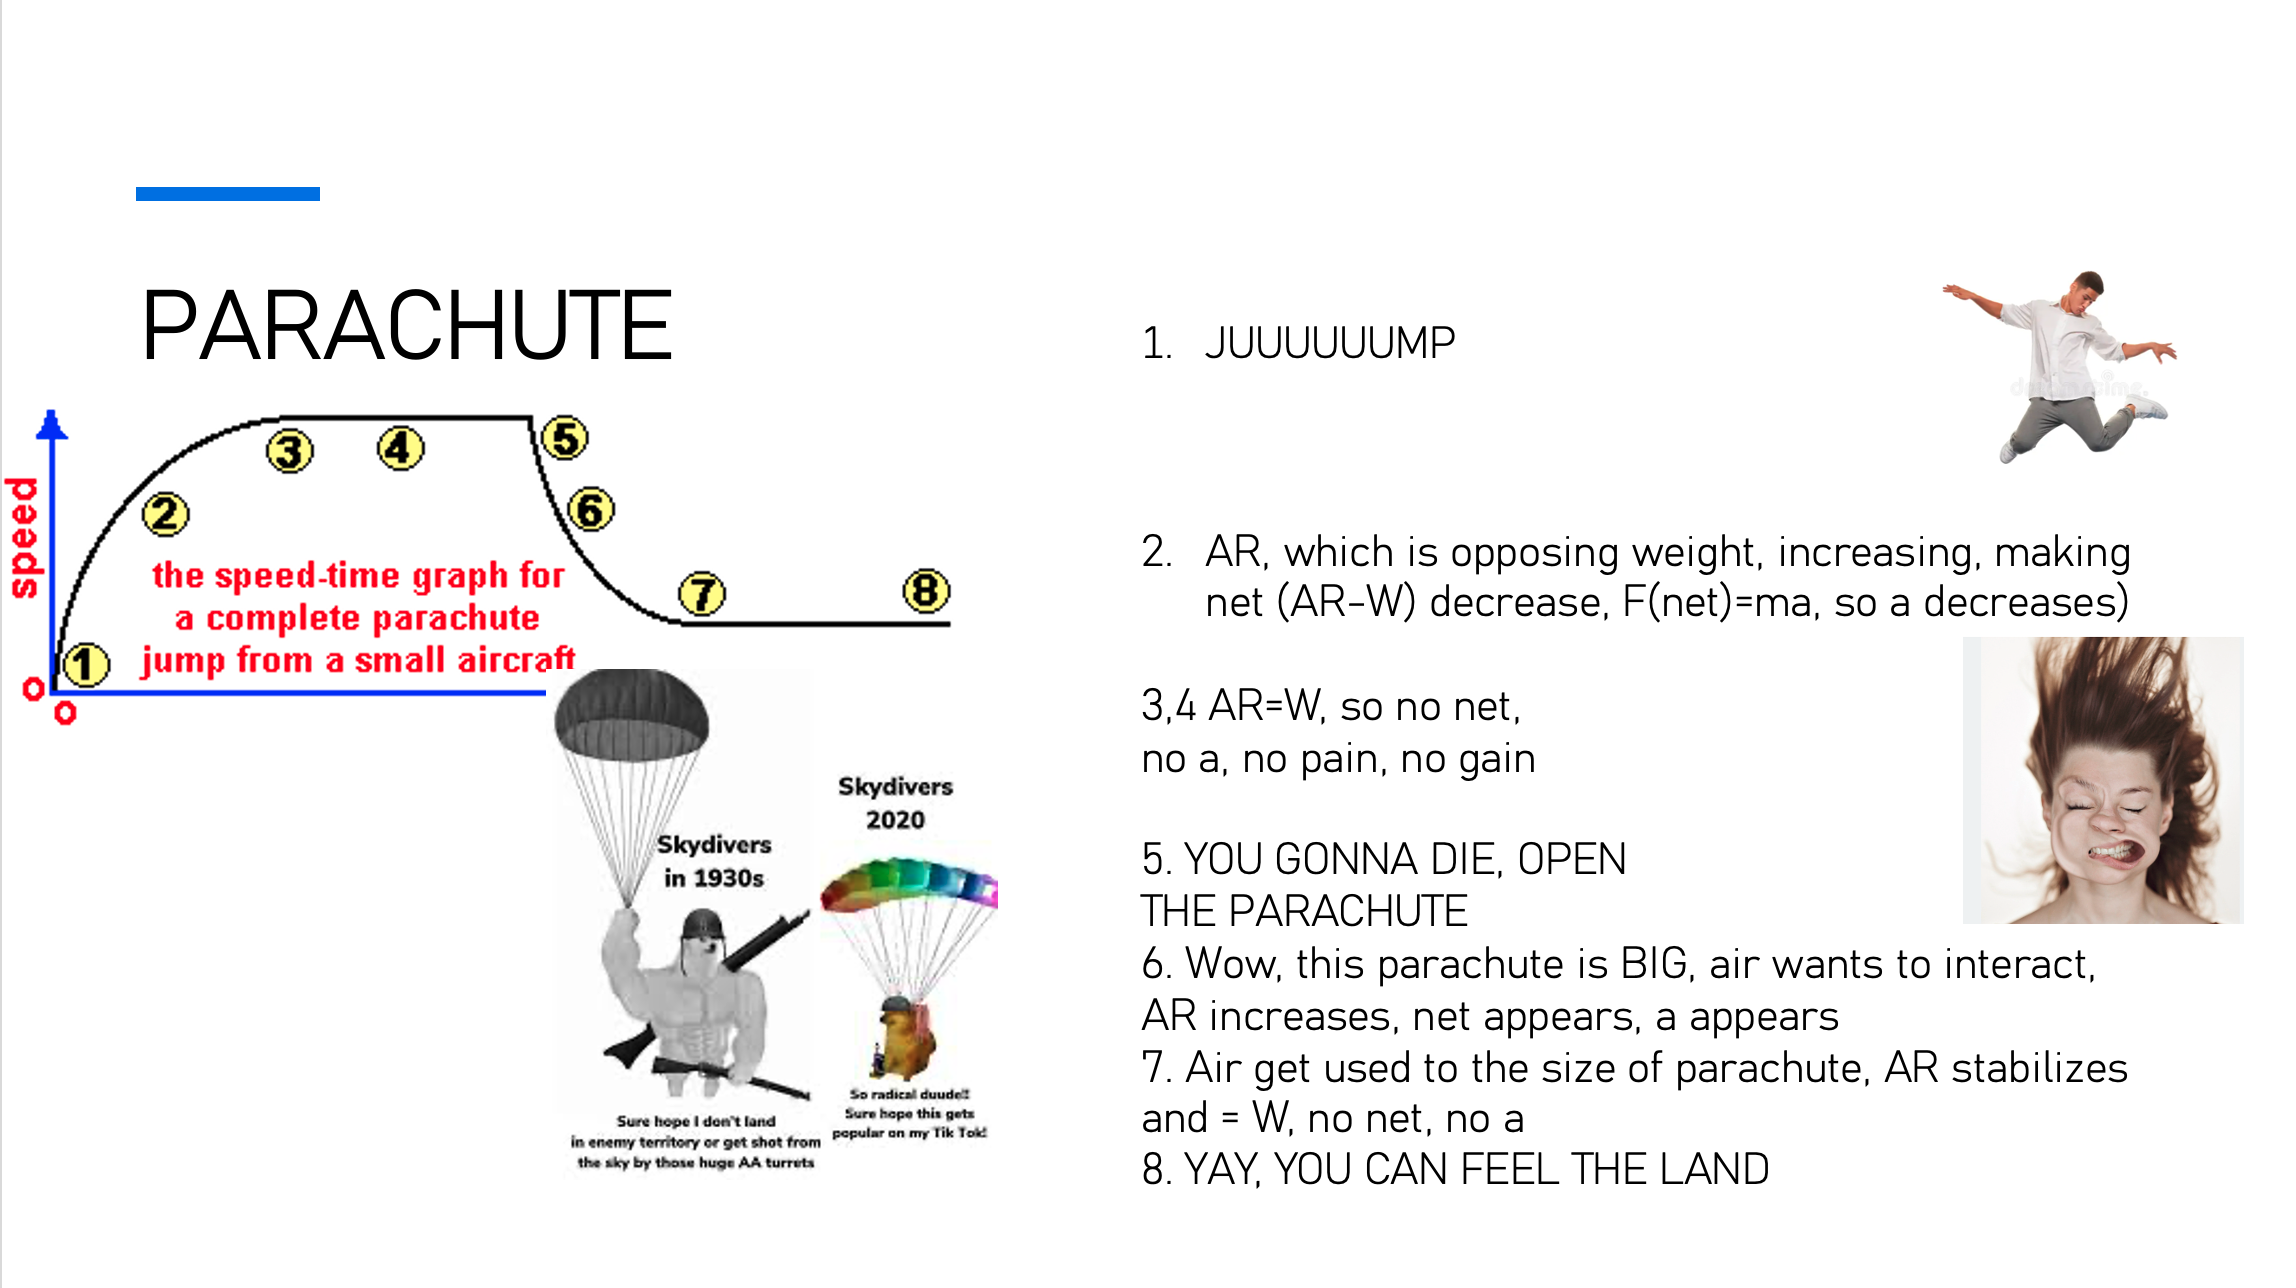
\includegraphics[width=1\linewidth]{1.png}\\
\(F_{res}=W-AR\).
\end{center}When \(W>AR, F_{res} \ne 0, a\ne 0;\) When \(W=AR, F_{res}=0, a=0;\) (Terminal velocity reached)
\subsection{Mass, Weight, Density}
Mass is defined as \textbf{a measure of the quantity of matter in an object at rest relative to the observer}. Weight is defined as \textbf{the force acting on an object with mass when placed in a gravitational field}. Gravitational field strength is defined as \textbf{the force per unit mass acting on an object in a gravitational field}.\\
Weight can be calculated using \(W=mg\), where \(m\) is the mass of the object.\\
As you can see from the definition:
\begin{center}
Mass is the same, it is not affected by gravitational field strength;\\
Weight can be changing due to the changing gravitational field strength.\\
\end{center}
Density is defined as \textbf{the mass per unit volume of a material}. It can be calculated using \(\rho = \frac{m}{V}\).\\
A gas is less dense than the same substance in liquid or solid form. (Hi chemistry)\\
Related formulas for calculating volume:
\[\frac{4}3 \pi r^3\ \text{for sphere;}\ d^3\ \text{for cube};\ \pi r^2l\ \text{for cylinder}\]
Whether an object floats or sinks depends on the relative densities of the object and the fluid it is submerged in:
\begin{itemize}
\item If the object is denser than the fluid, it will sink.
\item If the object is less dense than the fluid, it will float.
\end{itemize}
A liquid with a lower density will float on a liquid with a higher density if the liquids do not mix.
\subsection{Forces}
Force is defined as \textbf{a push or a pull that acts on an object due to the interaction with another object}. Force \textbf{can change an object's speed, direction, shape \& size.} \\\\
A \textbf{resultant force} (\(F_{res}\)) is a single force that describes all of the forces operating on a body. \\
When multiple forces act on one object, the forces can be combined to produce one net force that describes the combined action of all of the forces.
This single resultant force determines \textbf{the direction in which the object will move as a result of all of the forces \& the magnitude of the net force experienced by the object.}\\\\
\textbf{Forces are balanced} if multiple forces act in opposing directions with an equal magnitude in each direction. In other words, \(F_{res}=0,\ a=0\).\\\\
Newton's \(1^{st}\) Law states that:
\begin{center}
\textbf{Objects will remain at rest, or move with a constant velocity unless acted on by a resultant force}\\
\end{center}
Newton's \(2^{nd}\) Law states that:
\begin{center}
\textbf{The acceleration of an object is proportional to the resultant force acting on it and inversely proportional to the object's mass}
\end{center}
In simpler terms:
\[F=ma\]
Newton's \(3^{rd}\) Law states that:
\begin{center}
\textbf{For every action, there is an equal and opposite reaction.}
\end{center}
\subsection{Hooke's Law}
Hooke's Law states that:
\begin{center}
\textbf{The extension of an elastic object is directly proportional to the force applied, up to the limit of proportionality}
\end{center}
In simpler terms:
\(F=kx\), where \(F\) is the force applied, \(k\) is the spring constant, \(x\) is the extension. \\
The spring constant is the \textbf{force per unit extension}.\\\\
For the graph:
\begin{itemize}
\item Linear relationship, with \(\frac{1}{k}\) as the gradient
\item Non-linear relationship beyond the \textbf{limit of proportionality}
\end{itemize}
\subsection{Circular Motion}
\textbf{The velocity is always changing due to the change of direction, while the speed stays the same as it is a scalar quantity.}\\
For an object in circular motion, \textbf{the force is always directed towards the center of the circle.}\\
The force needed to make something follow a circular path depends on:
\begin{itemize}
    \item Mass of the object: \(m\) increase, \(F\) increase
    \item Speed of the object: \(v\) increase, \(F\) increase
    \item Radius of the circle: \(r\) decrease, \(F\) increase
\end{itemize}
\subsection{Friction}
Friction is a force that works in opposition to the motion of an object. Frictional forces slow down the motion of the object.\\
When friction occurs, energy is transferred by heating.
\subsection{Moments \& Center of gravity}
\textbf{The moment of a force is the turning effect produced when a force is exerted on an object.} Moment is defined as \textbf{the turning effect of a force.}\\
Equation: \[m=F\times d\]
The forces should be perpendicular to the distance from the pivot. \\\\
The principal of moments states that for a balanced object:
\[\text{clockwise moment} = \text{anticlockwise moment}\]
Equilibrium for an object is reached when \(F_{res}=0 \ /\ m_{res}=0\).\\\\
The center of gravity is defined as \textbf{the point through which the weight of an object acts.}
For a symmetrical object of uniform density, the center of gravity is located at the point of symmetry. An object is stable when its center of gravity lies above its base. If the line of action of the weight force lies outside the base of the object, there will be a resultant moment, and the body will topple.
\subsection{Momentum \& Impulse}
Objects with mass that is in motion have momentum. Equation:
\[p=m\times v\]
\textbf{In a closed system, the total momentum before an event is equal to the total momentum after the event.}\\
When an external resultant force acts on an object for a very short time and changes the object's motion, we call this impulse. Equation:
\[\text{impulse}=F\times \Delta t=\Delta p;\ F=\frac{\Delta p}{\Delta t}\]
\subsection{Energy, Work, Power}
\subsubsection{Energy}
Energy is a property of an object that is stored or transferred. \\Energy is stored in objects in different energy stores:
\begin{center}
    \begin{tabular}{|c|>{\centering\arraybackslash}p{0.66\linewidth}|}\hline
         \textbf{Types of energy stores} & \textbf{Description}\\\hline
         Kinetic, \(E_k\)& Moving objects have energy in their kinetic store\\\hline
         Gravitational, GPE& Objects gain energy in their gravitational potential store when they are lifted through a gravitational field\\\hline
         Elastic& Objects have energy in their elastic potential store if they are stretched, squashed or bent\\\hline
         Magnetic& Magnetic materials interacting with each other have energy in their magnetic store\\\hline
         Electrostatic& Objects with charge (like electrons and protons) interacting with one another have energy in their electrostatic store\\\hline
         Chemical& Chemical reactions transfer energy into or away from a substance's chemical store\\\hline
         Nuclear& Atomic nuclei release energy from their nuclear store during nuclear reactions\\\hline
         Thermal& All objects have energy in their thermal stores; the hotter the object, the more energy it has in this store\\\hline
    \end{tabular}
    \begin{tabular}{|c|>{\centering\arraybackslash}p{0.6\linewidth}|}\hline
        \textbf{Transfer Pathway of energy} & \textbf{Description}\\\hline
        Mechanical Working & When a force acts on an object (e.g. pulling, pushing, stretching, squashing)\\\hline
        Electrical working & A charge moving through a potential difference (e.g. current) \\\hline
        Heating (by particles) & Energy is transferred from a hotter object to a colder one (e.g. conduction) \\\hline
        (Heating by) radiation & Energy transferred by electromagnetic waves (e.g. visible light)\\\hline
    \end{tabular}
\end{center}
I directly copied these from SaveMyExams because I'm too lazy.\\\\
\textbf{Kinetic energy}, i.e. energy in an object's kinetic store, is defined as:
\begin{center}
The amount of energy an object has as a result of its mass and speed.
\end{center}
Equation:
\[E_k=\frac{1}2mv^2; E_k \propto m \ \& \ v^2\]
\textbf{Gravitational potential energy} is defined as:
\begin{center}
The energy an object has due to its height in a gravitational field.
\end{center}
Equation:
\[\Delta E_p=mg\Delta h\]
The principle of conservation of energy states that:
\begin{center}
\textbf{Energy cannot be created or destroyed, it can only be transferred from one store to another.}
Therefore, energy cannot be ‘lost’, but it can be transferred to the surroundings.
\end{center}
I don't want to waste time on Sankey diagrams. For those who don't know it, use Google!
\subsubsection{Work done}
Mechanical work is done when \textbf{an object is moved over a distance by a force applied in the direction of its displacement.} Equation:
\[W=F\times d=\Delta E\]
\subsubsection{Power}
Power is defined as \textbf{work done per unit time}. It is also equal to energy transferred per unit time. Equation:
\[P=\frac{W}t=\frac{\Delta E}t\]
Energy efficiency is defined as \textbf{the ratio of the useful power or energy output from a system to its total power or energy input}. Word equation:
\[\text{efficiency}=\frac{\text{useful output}}{\text{total input}}\times 100\%\]
\subsection{Energy Sources}
Only thing you need to remember for this part: energy sources \textbf{NOT derived from the sun!}
\begin{center}
Geothermal, Nuclear, Tidal
\end{center}
We already knew so much about advantages and disadvantages of renewable and non-renewable energy sources, so don't worry. 
\subsection{Pressure (in a nutshell)}
Defined as \textbf{the force per unit area}, formula:
\[p=\frac{F}A\ \text{for solids};\ \Delta p=\rho g\Delta h\ \text{for liquids.} \]
\newpage
\section{Thermal Physics}
\subsection{Kinetic Particle Model}
\begin{center}
    \begin{tabular}{|>{\centering\arraybackslash}p{0.3\linewidth}|>{\centering\arraybackslash}p{0.3\linewidth}|>{\centering\arraybackslash}p{0.3\linewidth}|}\hline
         \textbf{Solids}& \textbf{Liquids}& \textbf{Gases}\\\hline
         Definite shape \& volume&  No definite shape, definite volume& No definite shape / volume\\\hline
         Can't flow, incompressible&  Can flow, incompressible& Can flow, compressible\\\hline
         High Density& Medium Density & Low Density\\\hline
         Regular arrangement of particles & Random arrangement & Random arrangment\\\hline
         Particles vibrate around a fixed position & Particles vibrate and slide past each other & Particles move quickly in all directions \\\hline
         Low Energy Particles & Greater Energy Particles & Highest Energy Particles\\\hline
    \end{tabular}
\end{center}
List of \textit{professional vocabs} for change in states:
\begin{itemize}
    \item Melting
    \item Boiling
    \item Condensation
    \item Solidification
    \item Sublimation
    \item Deposition
\end{itemize}
Since we all learned chemistry, I'm not going to specify why intermolecular forces affect states of matter. Also I'm not explaining Kinetic Particle Theory in detail.\\\\
\textbf{Brownian motion is the random movement of particles} in a liquid or a gas produced by large numbers of collisions with smaller particles which are often too small to see. Why?
\begin{center}
These light, fast-moving atoms and molecules collide with the larger microscopic particles. The collisions give the particles a little nudge, causing them to change their speed and directions randomly, each time they are struck by a molecule. The presence of the light, fast moving atoms and molecules is inferred from the motion of the microscopic particles.
\end{center}
For particles in gases, molecules in a gas are in constant random motion \textbf{(Brownian Motion)} at high speeds. Pressure in a gas is caused by the collisions of particles with the walls of the container.
\[0\ K= -273.15\degree C\ \text{(I know no one cares)}\]
Key Gas Law you need to know:
\[\text{Boyle's Law:} p\propto \frac{1}{V};\ pV=k;\ p_1V_1=p_2V_2;\]
\[\text{An Ultimate Formula:}\ \frac{p_1V_1}{T_1}=\frac{p_2V_2}{T_2}, \text{where}\ p= \text{pressure}, V=\text{volume}, T=\text{temperature}\]
Explanation when asked about pressure increase: due to (some reasons), particles collide with the wall more frequently, increase rate of change in momentum, increase in force, increase in pressure. 
\subsection{Thermal Expansion, Specific Heat Capacity}
\subsubsection{Thermal Expansion}
When a material is heated at constant pressure, its temperature increases, overall volume increases, its density decreases. This expansion happens because the molecules start to vibrate faster as they gain kinetic energy, and this causes them to collide with each other more often and push each other apart.\\
Thermal expansion in solids, liquids and gases:
\begin{center}
\begin{tabular}{|>{\centering\arraybackslash}p{0.07\linewidth}|>{\centering\arraybackslash}p{0.25\linewidth}|>{\centering\arraybackslash}p{0.6\linewidth}|}\hline
    \textbf{Solid} & Expands slightly& The low energy molecules cannot overcome the intermolecular forces of attraction holding them together\\\hline
    \textbf{Liquid} & Expands more than solid& The molecules have enough energy to partially overcome the intermolecular forces of attraction holding them together\\\hline
    \textbf{Gas} & Expand significantly& The high energy molecules have enough energy to completely overcome the intermolecular forces of attraction holding them together\\\hline
\end{tabular}
\end{center}
Applications include liquid-in-glass thermometers \& temperature-activated switches (made from bimetallic strip). 
\subsubsection{Specific Heat Capacity / \(c_{sp}\)}
Specific Heat Capacity is defined as:\begin{center}
\textbf{The energy required per unit mass per unit temperature increase.}
\end{center}
In other words, this is the amount of energy required to raise the temperature of 1 kg of a substance by 1 \degree C. Equation:
\[c=\frac{\Delta E}{m\Delta \theta}.\ \Delta E\ \text{can be determined using}\ \Delta E=Pt.\]
\subsubsection{Evaporation}
I believe you know the difference between boiling and evaporation. Happens in a range of temperatures. Whole process in one sentence: particles with higher kinetic energy escape from the surface therefore average energy of liquid decreases causing cooling.
\begin{enumerate}
    \item The molecules in a liquid have a range of energies.
    \item Evaporation occurs when more energetic molecules moving near the surface of the liquid have enough energy to escape.
    \item The average energy of the liquid is reduced when the particles with most energy leave.
    \item Therefore liquids are cooled down by evaporation. (Cooling effect)
\end{enumerate}
Factors affecting evaporation: Temperature of the liquid, Surface area of the liquid, Air movement.
\subsection{Conduction, Convection, Radiation}
\subsubsection{Conduction}
Conduction is \textbf{the transfer of heat from one region to another through particle vibrations and the movement of free electrons.} Conduction is the main method of thermal energy transfer in solids. Conduction can occur through atomic vibrations and free electron collisions.\\\\
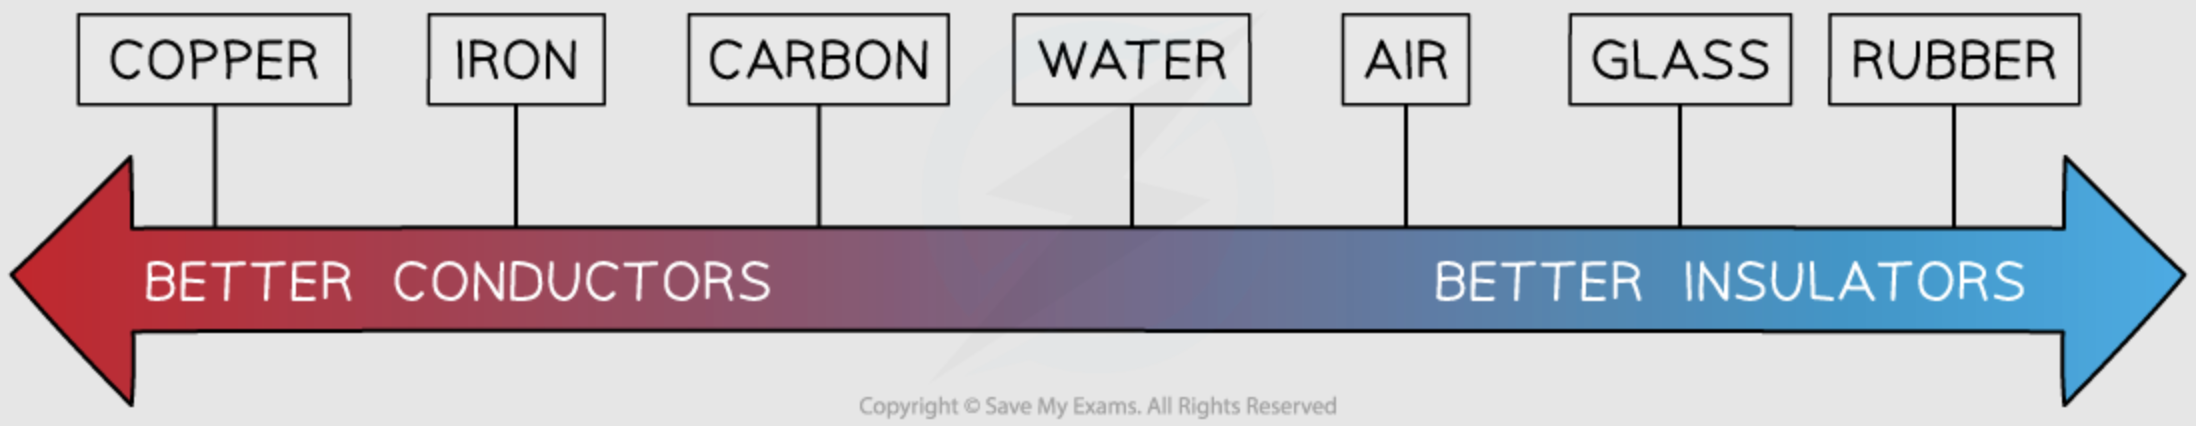
\includegraphics[width=1\linewidth]{截圖 2026-02-09 13.20.55.png}
\subsubsection{Convection}
Convection \textbf{ONLY happens in fluids, i.e. liquids \& gases.} \\Process of a convection current:
\begin{enumerate}
    \item When a liquid / gas is heated, the heated molecules vibrate and push each other apart, making the liquid / gas expand;
    \item This makes the hot liquid / gas less dense than the surroundings;
    \item The hot liquid / gas rises, and the cooler liquid / gas moves in to take its place;
    \item Eventually the hot liquid / gas cools and contracts, increasing in density, and sinks back down again.
\end{enumerate}
\subsubsection{Radiation}
\begin{center}\textbf{Thermal radiation = IR radiation.}\end{center}
Thermal radiation is the only way in which heat can travel through a vacuum; it does not need a medium to travel. Larger surface area and hotter surface emit more radiation. (Obviously)\\
Surface color and texture of the surface of the object determine the amount of thermal radiation emitted / absorbed by the object: \begin{center}Black / Dull = More radiation emitted \& absorbed;\\ White / Shiny = Less radiation emitted \& absorbed.
\end{center}
Objects will try to reach \textbf{Thermal Equilibrium}, a point where the object is absorbing energy at the same rate as it is emitting energy. At this point, the object has constant temperature. Energy taken from the surroundings is equal to the energy given to the surroundings.
\subsubsection{Applications}
I'm just going to provide a list for possible applications of thermal energy transfers:\\
(These include both applications of conduction and convection: see if you can identify!)
\begin{itemize}
    \item Metal pans
    \item Metal radiators
    \item Plastic handles of saucepans
    \item Double-glazed windows
    \item Heating room with radiator
    \item Steam rising which cools a hot liquid
\end{itemize}
\begin{center}
    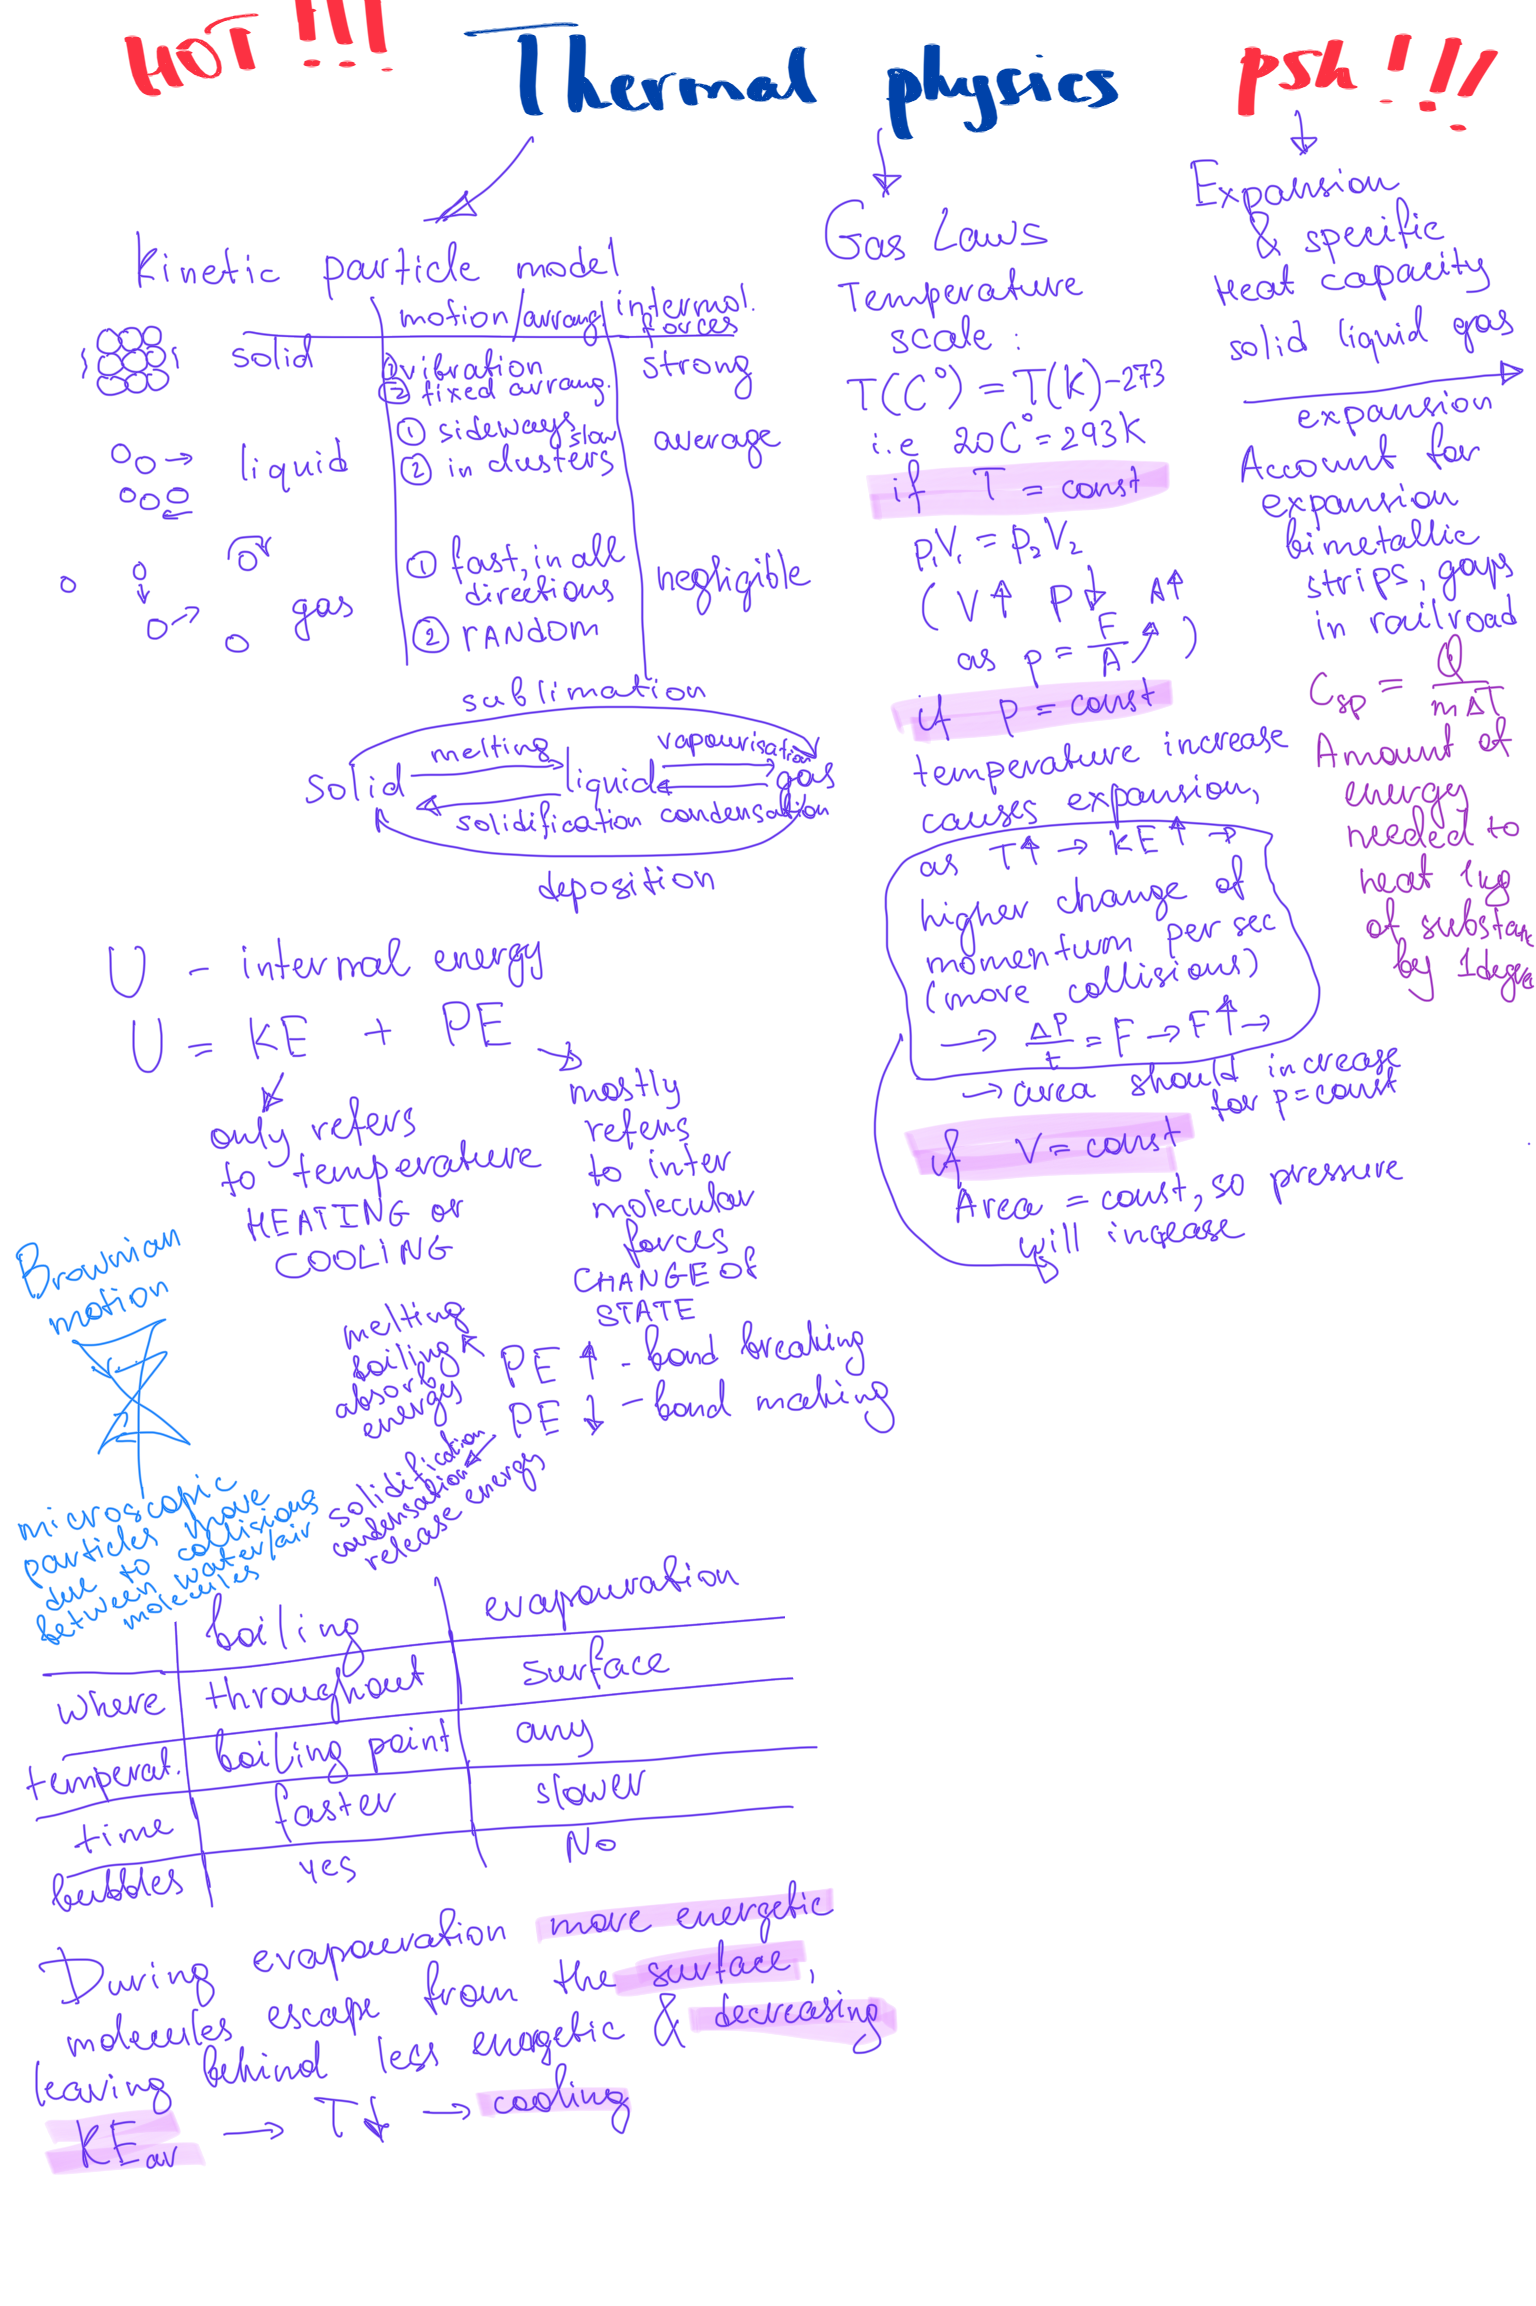
\includegraphics[width=1\linewidth]{overview, no heat transfers.png}
\end{center}

\section{Waves}
\begin{center}
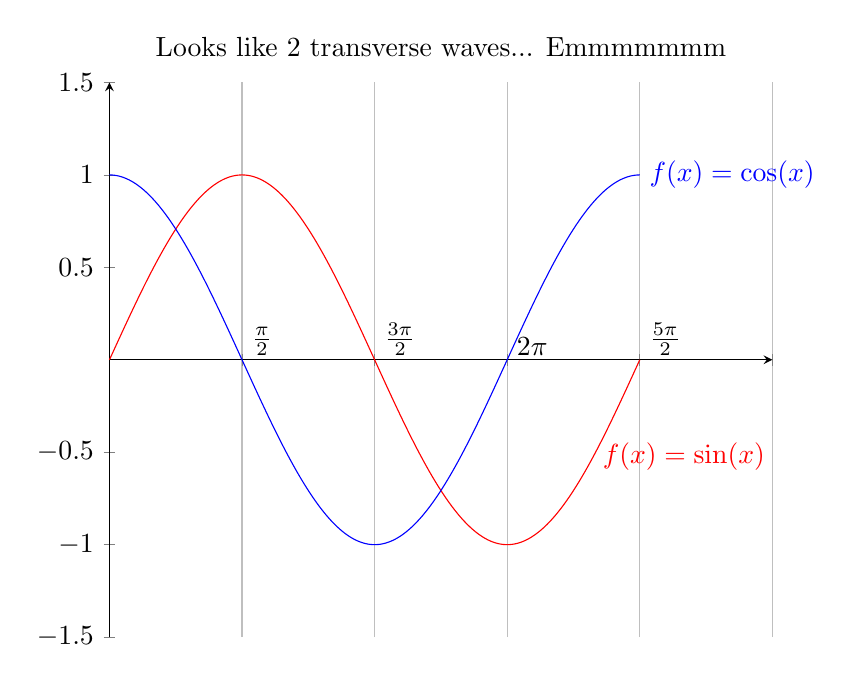
\begin{tikzpicture}
    \begin{axis}[
        clip=false,
        xmin=0,
        xmax=2.5*pi,
        ymin=-1.5,
        ymax=1.5,
        axis lines=middle,
        xtick={0,pi/2,pi,3*pi/2,2*pi,5/2*pi},
        xticklabels={$0$,$\frac{\pi}{2}$,$\frac{3\pi}{2}$,$2\pi$,$\frac{5\pi}{2}$},
        xticklabel style={anchor=south west},
        xmajorgrids=true,
        title={Looks like 2 transverse waves... Emmmmmmm}
    ]
        \addplot[domain=0:2*pi,red,samples=360]{sin(deg(x))}
        node[right,pos=0.9]{$f(x)=\sin (x)$};
        \addplot[domain=0:2*pi,blue,samples=360]{cos(deg(x))}
        node[right,pos=1]{$f(x)=\cos (x)$};
    \end{axis}
\end{tikzpicture}
\end{center}
\subsection{General Properties of Waves}
Waves transfer energy without transferring matter. Waves are described as oscillations or vibrations about a fixed point. Key \textit{professional vocabs} you need to know when describing a wave:
\begin{itemize}
    \item Types of waves: \textbf{Transverse or Longitudinal?}
    \begin{itemize}
        \item \textbf{Transverse waves:} Waves where the direction of vibration is at right angles to the direction of energy transfer. For a transverse wave, the oscillation is perpendicular to the direction the wave is traveling in.
        \item \textbf{Longitudinal waves:} Waves where the direction of vibration is parallel to the direction of propagation. The energy transfer is in the same direction as the wave motion.
    \end{itemize}
    \item Wavefront
    \begin{itemize}
        \item Useful way of picturing waves from above
        \item Each wavefront, drawn as a single line, is used to represent a single wave
        \item The arrow shows the direction the wave is moving.
        \item The space between each wavefront represents the wavelength \(\lambda\).
    \end{itemize}
    \item Amplitude, \(A\)
    \begin{itemize}
        \item Defined as the maximum displacement of a wave from its undisturbed position.
        \item In other terms: Distance between undisturbed position to crest / trough.
    \end{itemize}
    \item Wavelength, \(\lambda\)
    \begin{itemize}
        \item Defined as the distance from one point on the wave to the same point on the next wave
        \item For transverse waves, \(\lambda\) can be measured from one peak to the next peak.
        \item For longitudinal waves, \(\lambda\) can be measured from the center of one compression to the center of the next.
    \end{itemize}
    \item Frequency, \(f\ (Hz)\), the number of waves passing a point in a second
    \item Period, \(T\ (s)=\frac{1}{f}\), the time taken for one complete oscillation to pass a fixed point
    \item Crest \& Trough / Compression \& Rarefaction
    \begin{itemize}
        \item Crest: The highest point on a wave above its undisturbed position
        \item Trough: The lowest point on a wave below its undisturbed position
        \item Compression: a region of higher density i.e. a place where the molecules are bunched together
        \item Rarefaction: a region of lower density i.e. a place where the molecules are spread out
    \end{itemize}
    \item Wave speed, \(v\ (m/s)\), the distance traveled by a wave each second, given by \textbf{\(v=f\lambda\)}
    \item Behaviors undergone:
    \begin{itemize}
        \item \textbf{Reflection} when a wave hits a boundary between two media at a plane surface and does not pass through, but instead stays in the original medium
        \item \textbf{Refraction} when a wave passes a boundary between two different transparent media and undergoes a change in \(v,\lambda\), direction.
        \begin{itemize}
            \item Information you need to know: The water surface waves slow down when passing from deep to shallow water in the ripple tank.
        \end{itemize}
        \item \textbf{Diffraction} when waves pass through a narrow gap, the waves spread out;
        \begin{itemize}
            \item The extent of diffraction depends on the width of the gap compared with the wavelength of the waves.
            \item Shorter wavelengths undergo less diffraction than longer wavelengths.
            \item For drawing question, draw either semi-circles / bracket-like (quarter-circle (?) + straight lines) shapes depending on the \(\lambda\) and the gap size.
        \end{itemize}
    \end{itemize}
\end{itemize}
\subsection{Light, Lens, Refraction, TIR, Dispersion}
\subsubsection{Info on how to draw ray diagrams}
\textbf{Reflection}
\begin{itemize}
\item A normal line is drawn at right angles to the boundary between two media.
\item The angle of the wave approaching the boundary is called the angle of incidence \(\angle i\).
\item The angle of the wave leaving the boundary is called the angle of reflection \(\angle r\).
\item An incident ray has an arrow pointing towards the boundary.
\item A reflected ray has an arrow pointing away from the boundary.
\end{itemize}
\begin{center}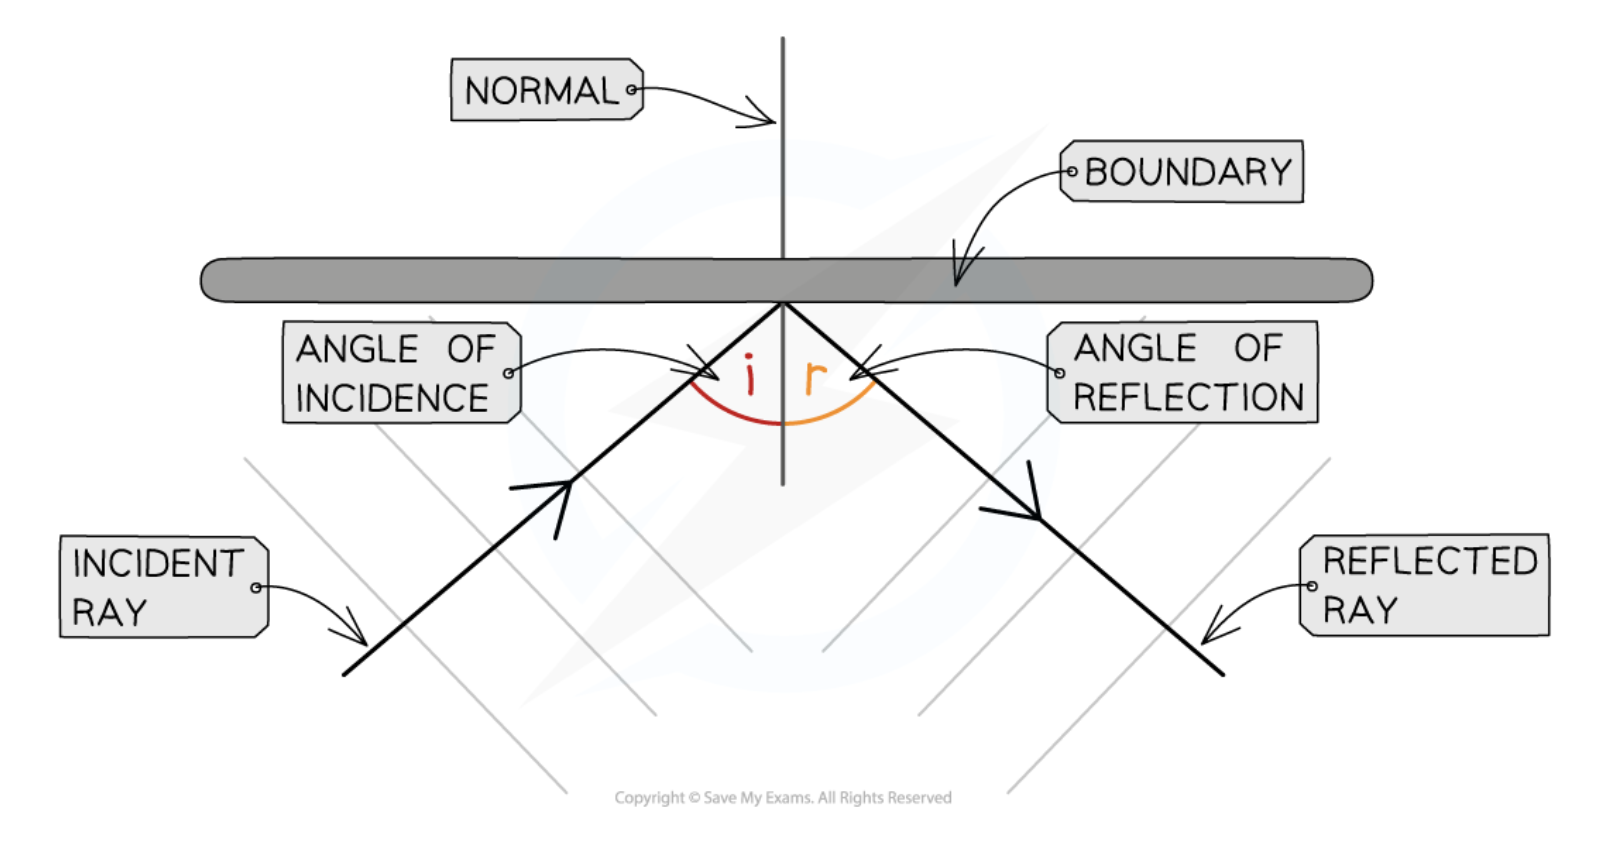
\includegraphics[width=0.5\linewidth]{截圖 2026-02-09 15.08.21.png}\end{center}
\begin{center}
    \textbf{\(i=r\), angle of incidence = angle of reflection} (make sure you include this in the drawing!)
\end{center}
\textbf{Reflection (Mirror)}\\\\
When an object is placed in front of a plane mirror, an image of that object can be seen in the mirror. The image will be the same size as the object, the same distance behind the mirror as the object is in front of it, and \textbf{virtual}.
\\\\Each incident ray on the diagram above can be drawn following these steps:
    \begin{itemize}
        \item Light from the object hits the mirror, reflecting from it (i=r)
        \item To an observer, the reflected ray appears to have come from behind the mirror
        \item The reflected ray can be traced back in this same direction behind the mirror, forming a virtual ray
        \item This process is repeated for another ray traveling in a slightly different direction
        \item An image of the object will appear where these two virtual rays cross
    \end{itemize}
\begin{center}
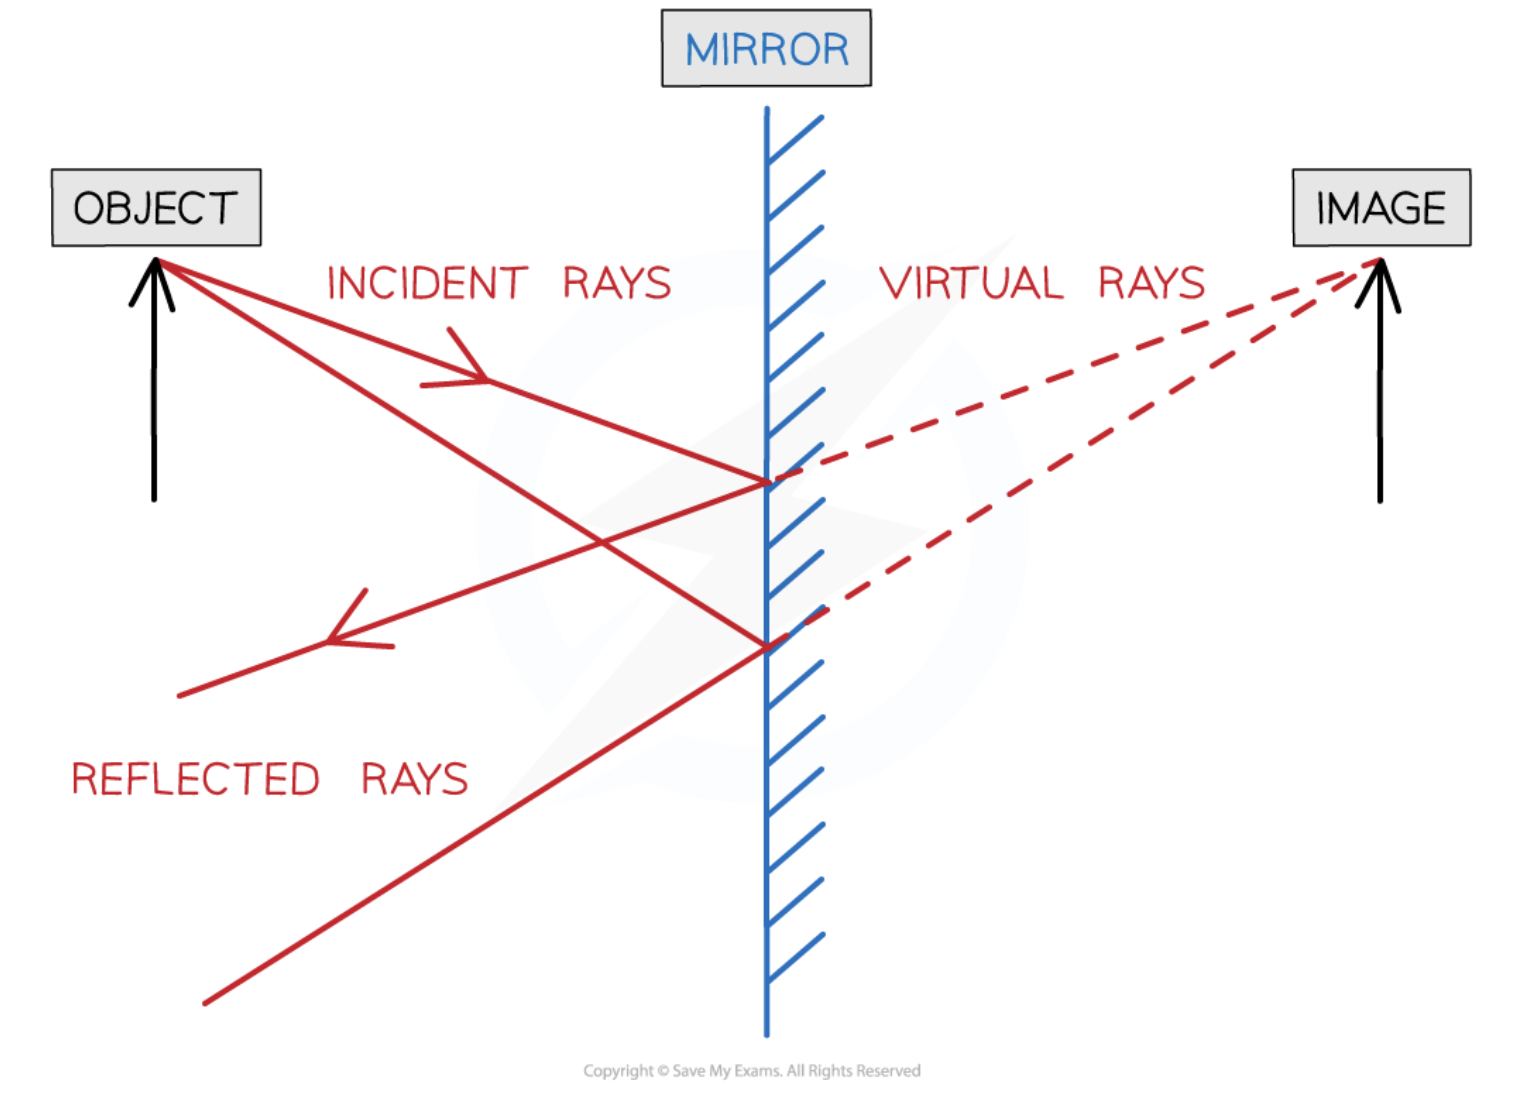
\includegraphics[width=0.7\linewidth]{截圖 2026-02-09 15.15.43.png}
\end{center}
\textbf{Refraction}
\begin{itemize}
    \item In refraction, angles are measured between the ray (showing the direction of the wave) and the normal line.
    \item The angle of the wave approaching the boundary is called the angle of incidence \(\angle i\).
    \item The angle of the wave leaving the boundary is called the angle of refraction \(\angle r\).
    \item When drawing a ray diagram an arrow is used to show the direction the wave is traveling.
    \item An incident ray has an arrow pointing towards the boundary.
    \item A refracted ray has an arrow pointing away from the boundary.
\end{itemize}
\begin{center}
    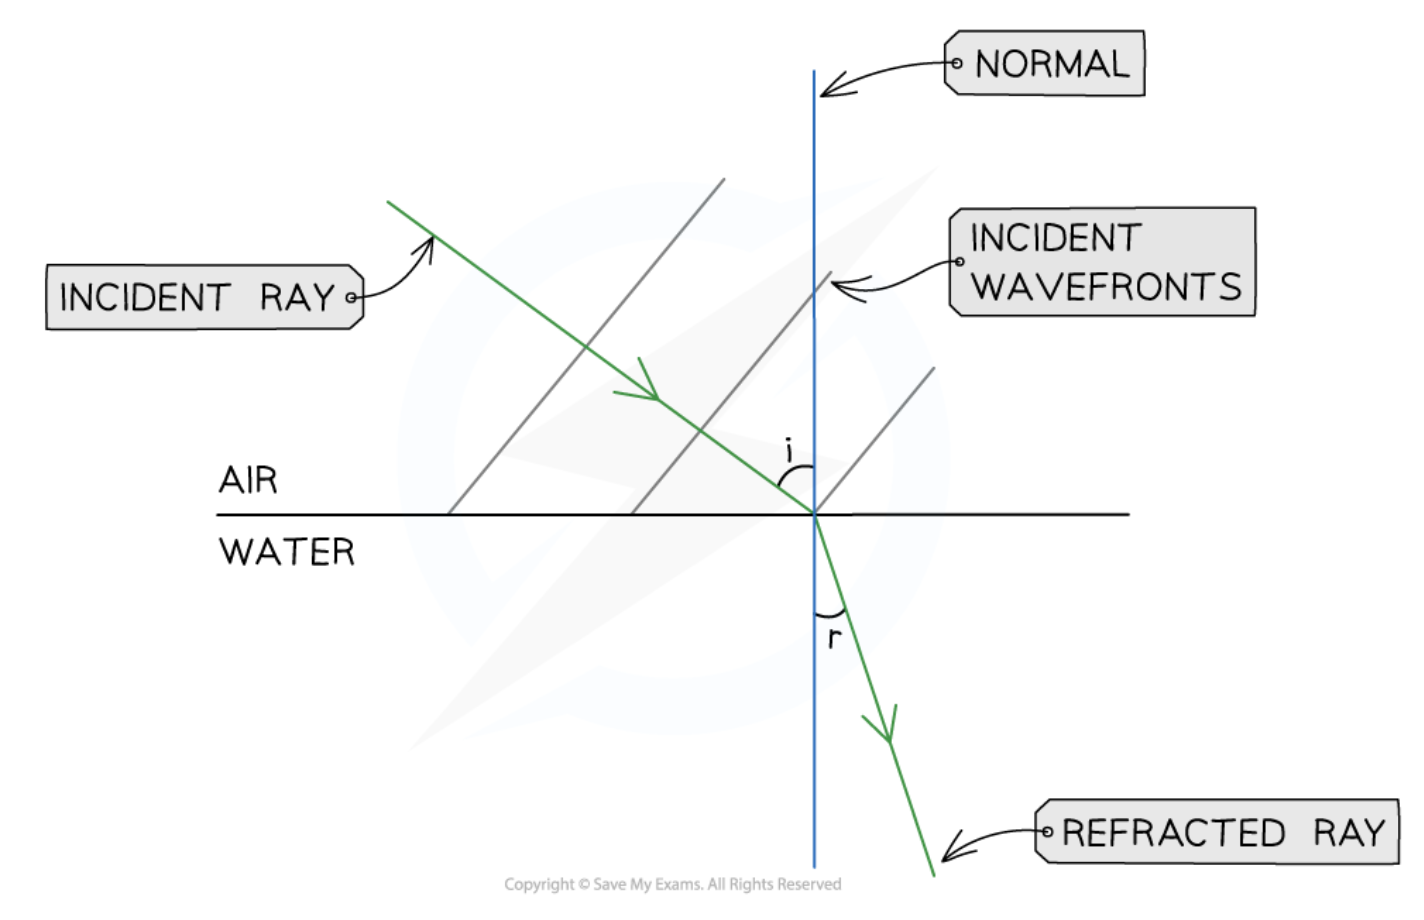
\includegraphics[width=0.7\linewidth]{截圖 2026-02-09 15.21.46.png}
\end{center}
\textbf{Refraction (Air to glass block)}
\begin{center}
    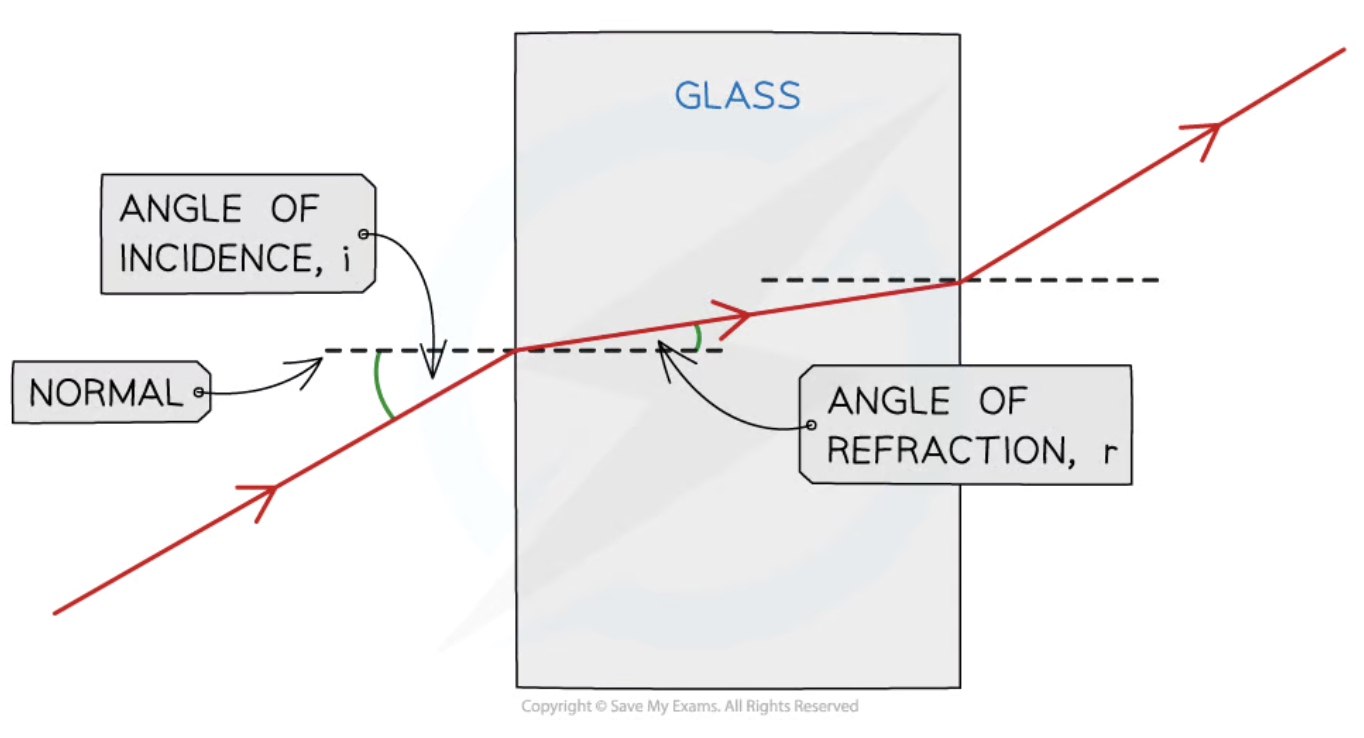
\includegraphics[width=0.7\linewidth]{截圖 2026-02-09 15.24.02.png}
\end{center}
\textbf{Converging Lens}\\\\
In a converging lens, parallel rays of light are brought to a focus. \\This point is called the principal focus. \\
The distance from the lens to the principal focus is called the focal length. \\
The more curved the lens, the shorter the focal length.
\begin{center}
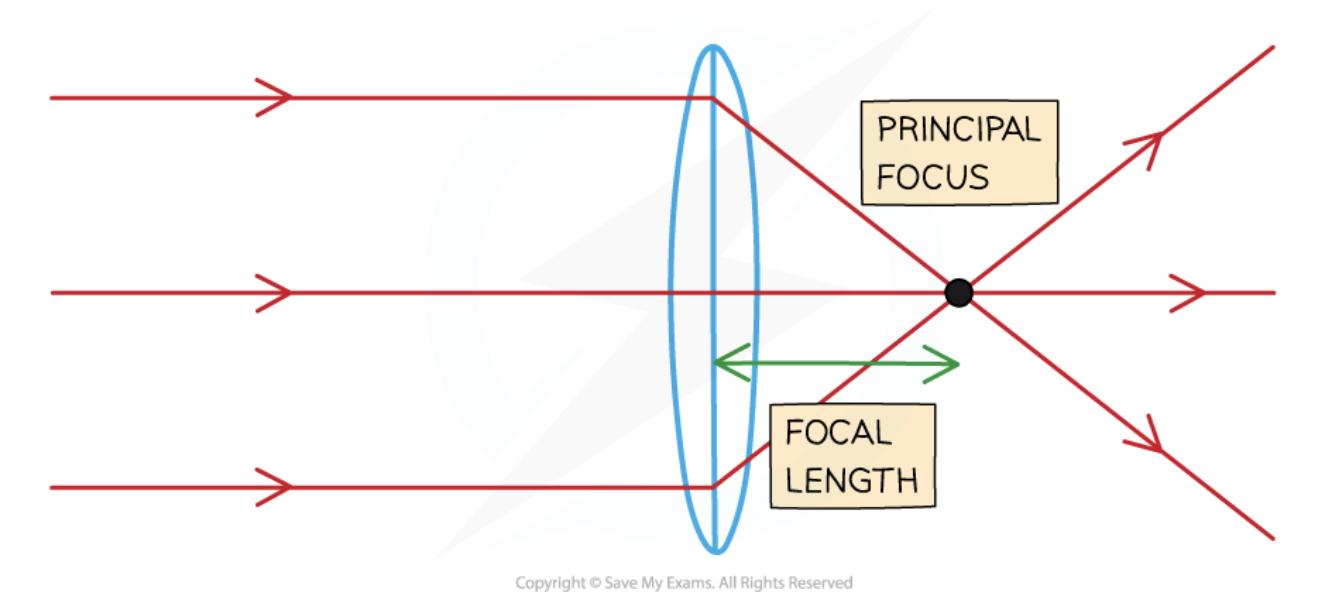
\includegraphics[width=0.7\linewidth]{截圖 2026-02-09 15.37.05.png}\\
\end{center}
\textbf{Converging Lens Continued: Converging ray diagrams}\\
\begin{enumerate}
    \item Rays passing through the principal axis will pass through the optical centre of the lens undeviated.
    \item Rays that are parallel to the principal axis will be refracted and pass through the focal point \(f\).
    \item Rays passing through the focal point f will emerge parallel to the principal axis.
\end{enumerate}
\begin{center}
    \begin{tabular}{|c|c|c|c|c|}\hline
        \textbf{Object Position} & \textbf{Image Position} & \textbf{Image Type} & \textbf{Orientation of image} & \textbf{Size of image}\\\hline
         \(>2f\)&  \(f<\text{pos}<2f\)&  Real&  Inverted& Diminished\\\hline
         \(2f\)&  \(2f\)&  Real&  Inverted& Same\\\hline
         \(f<\text{pos}<2f\)&  \(>2f\)&  Real&  Inverted& Magnified\\\hline
 \(f\)& \(\infty\)& & &\\\hline
         \(<f\)&  \(2f\)&  Virtual&  Upright& Magnified\\ \hline
    \end{tabular}
\end{center}
\textbf{Diverging Lens}\\\\
In a diverging lens, parallel rays of light are made to diverge (spread out) from a point.\\
The principal focus is now the point from which the rays appear to diverge from.\\
\begin{center}
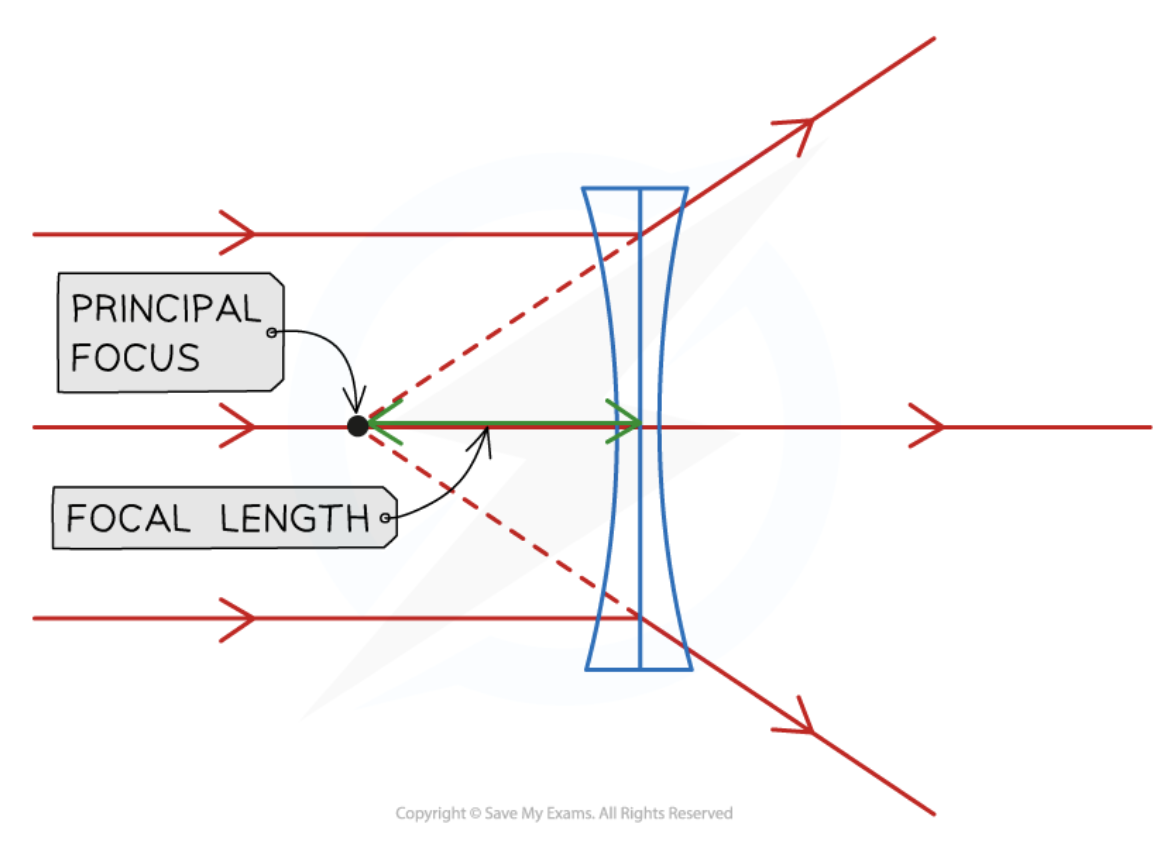
\includegraphics[width=0.7\linewidth]{截圖 2026-02-09 15.37.16.png}
\end{center}
\textbf{Diverging Lens continued: Diverging rays}\\
All images formed by diverging lens are:
\begin{itemize}
    \item Virtual
    \item Upright
    \item Diminished
    \item On the same side of the lens as the object
\end{itemize}
You are not required to draw a diverging rays diagram.
\subsubsection{Refractive index}
The refractive index, \(n\), is defined as the ratio of the speeds of a wave in two different regions / the ratio of the sine of the angle of incidence and the sine of the angle of refraction of a wave in two different regions. Equation:
\[n=\frac{v\ \text{of light in vacuum}}{v\ \text{of light in material}}=\frac{\sin i}{\sin r}\]
\subsubsection{Total Internal Reflection, TIR}
TIR occurs at the boundary between two media when all the incident ray in medium 1 is reflected back into medium 1. For TIR to occur, the incident material must be denser than the second material. \\\\
Applications of TIR include periscopes \&  \textbf{Optic fiber} (let's go CS)\\\\
When the angle of refraction is exactly 90° the light is refracted along the boundary. At this point, the angle of incidence is known as\textbf{ the critical angle \(c\).} Equation:
\[c=\sin^{-1}(\frac{1}{n}); n=\frac{1}{\sin c}\]
\subsubsection{Real \& Virtual Images}
Images can be described compared to their object as:
\begin{itemize}
    \item Enlarged / same size / diminished
    \item Upright / Inverted
    \item Real / Virtual
\end{itemize}
A real image is defined as an image that is formed when the light rays from an object converge and meet each other and can be projected onto a screen. Real images are always inverted.\\\\
A virtual image is defined as an image that is formed when the light rays from an object do not meet but appear to meet behind the lens and cannot be projected onto a screen. A virtual image is formed by the divergence of light away from a point. Virtual images are always upright. \\\\
\textbf{Applications of lenses in correcting sight}
\begin{itemize}
    \item Converging lenses can be used to correct long-sighted vision.
    \item Diverging lenses can be used to correct short-sighted vision.
\end{itemize}
\subsubsection{Dispersion}
The dispersion of light is illustrated by the refraction of white light by a glass prism.\\
White light contains the wavelengths of all the colors of the spectrum. Each color has a different wavelength (and frequency), making up a very narrow part of the electromagnetic spectrum. White light may be separated into all its colors by passing it through a glass prism.\\
\textbf{Violet light is refracted the most, whilst red light is refracted the least.} \\(You better memorize it)\\\\
Q from Ms. Lydia: What is monochromatic light(, Kenny)?\\
A: Light with single \(f\) / frequency. Make sure not to say \textit{color} or else Ms. Lydia's going to kill you!
\\
\subsection{EM Spectrum}
The electromagnetic spectrum is arranged in a specific order based on the wavelengths or frequencies of the radiation in each region. Generally, longer wavelength \(\lambda\) means shorter frequency \(f\).\\ The speed of electromagnetic waves in a vacuum is \(3.0\times 10^8\ m/s\).
Main regions of EM spectrum (in order of decreasing \(\lambda\)) and their uses \& harms are:
\begin{itemize}
    \item Radio waves
    \begin{itemize}
        \item Radio and television transmissions
        \item Astronomy
        \item Radio frequency identification (RFID)
        \item Bluetooth
    \end{itemize}
    \item Microwaves
    \begin{itemize}
        \item Satellite television
        \begin{itemize}
            \item Geostationary satelites
            \item Low orbit satelites
        \end{itemize}
        \item Mobile (cell) phones
        \item Microwave ovens
        \item \textbf{Harms: Internal heating of body cells}
    \end{itemize}
    \item Infrared
    \begin{itemize}
        \item Television remote controllers
        \item Intruder alarms
        \item Thermal Imaging
        \item \textbf{Optic Fiber} (let's go CS)
        \item \textbf{Harms: Skin burns}
    \end{itemize}
    \item Visible Light
    \begin{itemize}
        \item Vision
        \item Photography
        \item Illumination
    \end{itemize}
    \item Ultraviolet Light
    \begin{itemize}
        \item Security marking
        \item Detecting fake bank notes
        \item Sterilizing water
        \item \textbf{Harms: Damage to surface cells and eyes leads to skin cancer and eye conditions}
    \end{itemize}
    \item X-Ray
    \begin{itemize}
        \item Medical scanning
        \item Security scanners
        \item \textbf{Mutation or damage to cells in the body}
    \end{itemize}
    \item Gamma \(\gamma\) Rays
    \begin{itemize}
        \item Sterilising food and medical equipment
        \item Detection and treatment of cancer
        \item \textbf{Mutation or damage to cells in the body}
    \end{itemize}
\end{itemize}
\textbf{Digital \& Analog signals}\\\\
Analogue signals vary continuously: they can take any value.\\
A digital signal can only take one of two (discrete) states.
\subsection{Sound}
Sound waves are produced by vibrating sources. Sound waves are longitudinal, so a medium is needed to transmit sound waves. When a sound wave comes into contact with a solid, the longitudinal wave vibrations are transferred to the solid. 
\begin{itemize}
    \item Speed of sound in air: 330 to 350 m/s
    \item Speed of sound in liquids: around 1500 m/s
    \item Speed of sound in solids: around 5000 m/s
\end{itemize}
The frequency of a sound wave is related to its pitch. 
\begin{itemize}
    \item Sounds with a high pitch have a high frequency (or short wavelength).
    \item Sounds with a low pitch have a low frequency (or long wavelength).
\end{itemize}
The amplitude of a sound wave is related to its volume.
\begin{itemize}
    \item Sounds with a large amplitude have a high volume.
    \item Sounds with a small amplitude have a low volume.
\end{itemize}
Sound waves reflect off hard surfaces; the reflection of a sound wave is called an echo.\\\\
The human hearing range is \(20\ \text{to}\ 20000\ \text{Hz}\). \\\\
Ultrasound is defined as sound with a frequency higher than \(20\ \text{kHz}\). \\Ultrasound can be used in non-destructive testing of materials; medical scanning of soft tissue; and sonar. 
\newpage
\section{Electricity \& Magnetism (EM for short)}
\subsection{Magnetism \& Magnetic Fields}
The ends of a magnet are called poles. Magnets have north, \(N\), and south, \(S\), poles.\\
Magnetic forces are strongest at the poles. 
\begin{center}Like poles repel, opposite poles attract. \end{center}
Uses of permanent magnets include:
\begin{itemize}
    \item Compasses
    \item School Lab Experiments (Cambridge what the fuck is that???)
    \item Toys
    \item Fridge Magnets
\end{itemize}
Uses of electromagnets include:
\begin{itemize}
    \item MRI scanners
    \item Speakers and earphones
    \item Recycling
    \item Mag-lev trains
\end{itemize}
Magnetic metals include: \textbf{Iron, Cobalt, Nickel, Steel}, which can be attracted to either poles of the magnet. 
Using this characteristics, bringing a material close to a known magnet will determine if the material is magnetic, non-magnetic or if it is a magnet itself.
\\\\
There are two types of magnets: 
\begin{itemize}
    \item Permanent Magnets
    \begin{itemize}
        \item Permanent magnets are made out of permanent magnetic materials, like \textbf{steel}
        \item A permanent magnet will produce its own magnetic field
        \item It will not lose its magnetism
    \end{itemize}
    \item Temporary / induced magnets / magnetism
    \begin{itemize}
        \item A material with a soft iron core that becomes a magnet temporarily when it is placed in a magnetic field.
        \item Induced magnetism always causes a force of attraction between the permanent magnet creating the magnetic field and the induced magnet.
        \item The end of the material closest to the magnet will have the opposite pole to that of the magnet pole closest to the material.
        \item When removed from the magnetic field, the material will lose its induced magnetism quickly and become unmagnetised.
    \end{itemize}
\end{itemize}
\textbf{A magnetic field is defined as:}\begin{center} \textbf{a region in which a magnetic pole experiences a force.}\end{center}
\textbf{How to draw a magnetic field (diagram)}\\\\
The magnetic field is strongest at the poles. Therefore, the magnetic field lines are closer together at the ends of the magnets.\\
The magnetic field becomes weaker as the distance from the magnet increases. Therefore, the magnetic field lines get further apart.\\
Field lines always have an arrow indicating the direction of the field line. 
The direction of the field line shows the direction that the magnetic force would act, and the field lines always go from a north pole to a south pole.\\
\begin{center}
    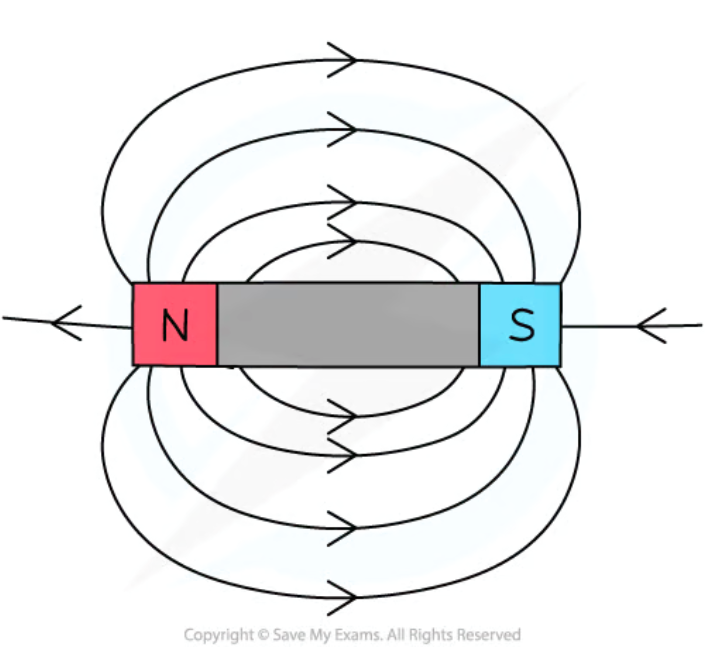
\includegraphics[width=0.5\linewidth]{截圖 2026-02-10 15.41.57.png}\\
\end{center}
\textbf{Attractive and Repulsive Magnetic Fields}
\begin{center}
    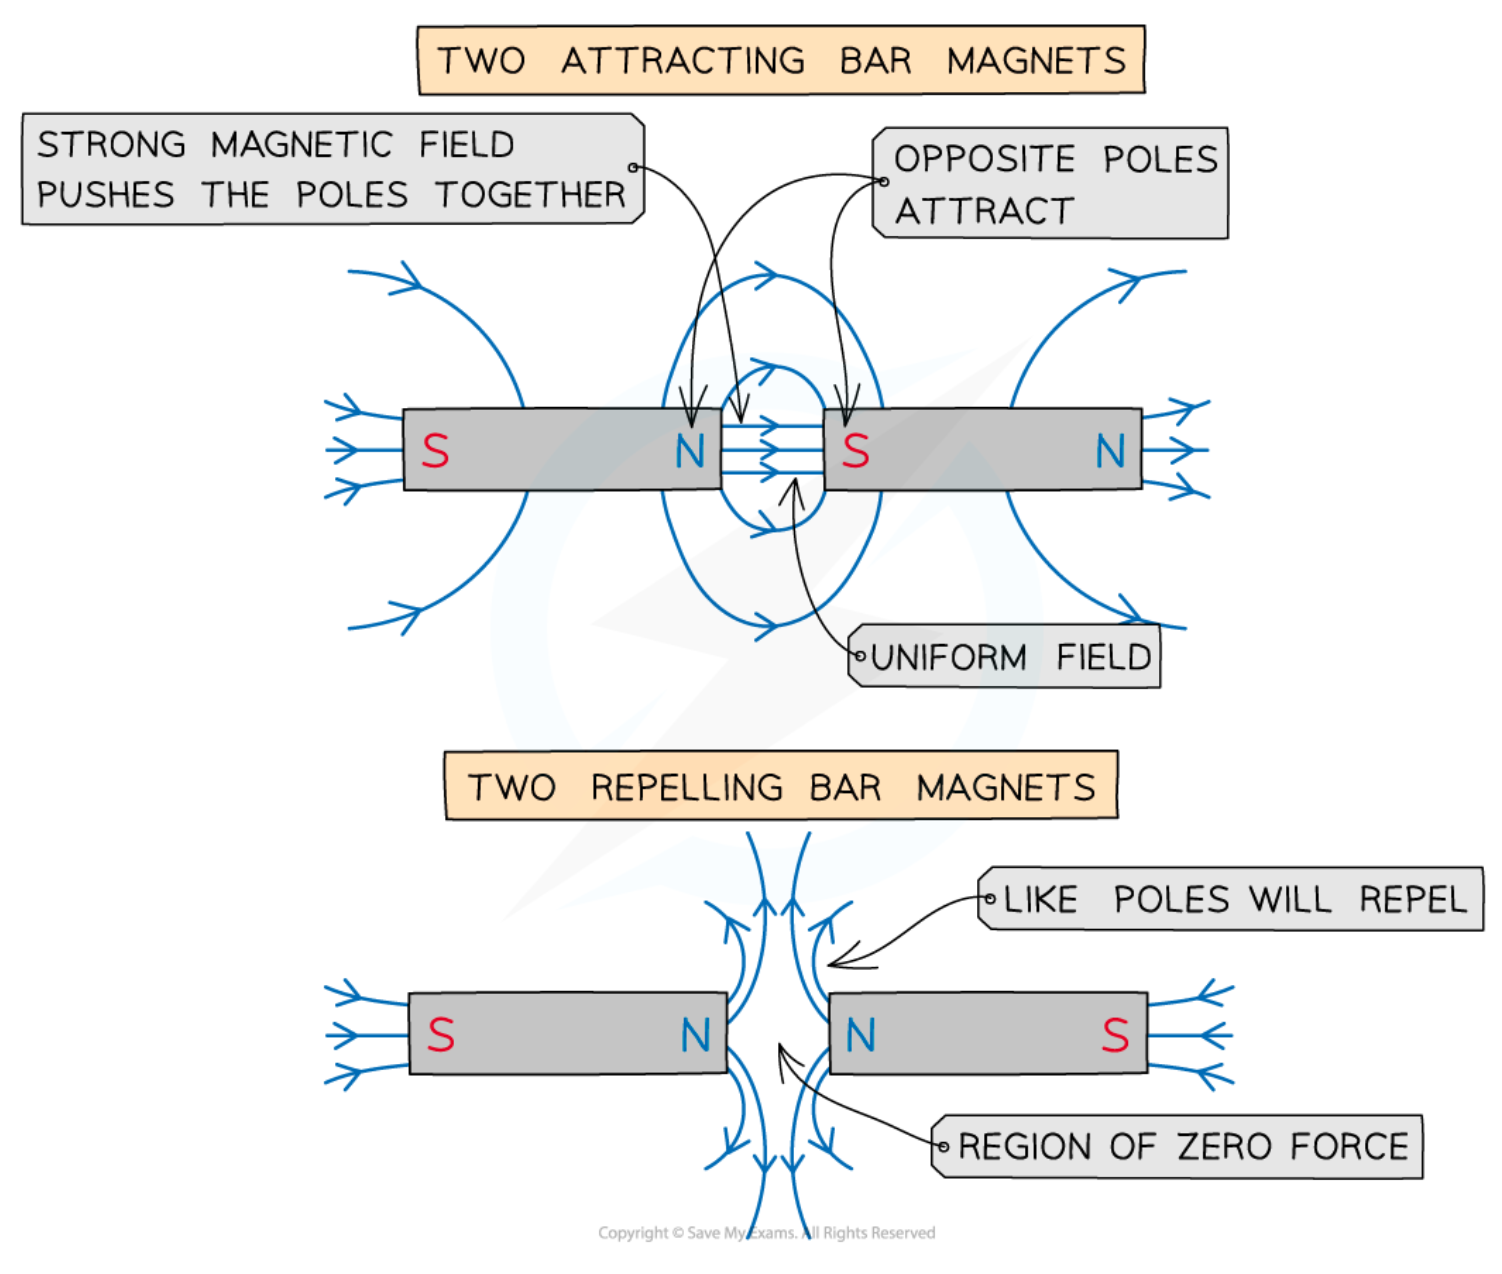
\includegraphics[width=0.7\linewidth]{截圖 2026-02-10 15.45.15.png}
\end{center}
When you're ask to do so, use \textbf{iron filings \& plotting compasses} to determine the magnetic field of an object.
\subsection{Electrical Quantities}
\subsubsection{Electric Charge, Electric Fields}
I'm not going to explain the structure of an atom. \\
Opposite charges attract, like charges repel. (I'm stating this just in case)\\
Electric charge is measured in units called coulombs \((C)\).\\\\
When certain insulating solids are rubbed against each other, they can become electrically charged. This is called charging by friction. 
The charges remain on the insulators and cannot immediately flow away. One gains a net positive charge and the other gains a net negative charge. Why? See below:
\begin{center}
    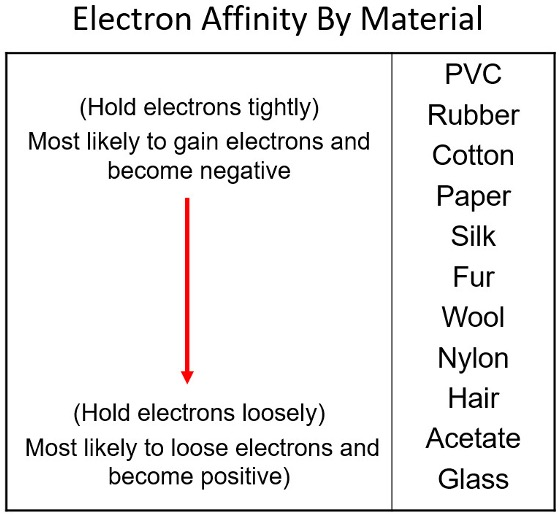
\includegraphics[width=0.5\linewidth]{图片 10.jpg}
\end{center}
A classic apparatus that can demonstrate the charge of the object is \textbf{the gold-leaf electroscope}.\\\\
An electric field is defined as:
\begin{center}
    \textbf{A region of space in which an electric charge experiences a force,}
\end{center}
while the direction of an electric field at a point is defined as the direction of the force on a positive charge at that point. \\
Charged objects create electric fields around themselves, and the electric field is a vector quantity.\\\\
\textbf{Electric Field Lines / Diagrams}\\\\
Around a point charge, the electric field lines are directly radially inwards or outwards:
\begin{itemize}
    \item If the charge is positive (+), the field lines are radially outwards.
    \item If the charge is negative (-), the field lines are radially inwards.
\end{itemize}
\begin{center}
    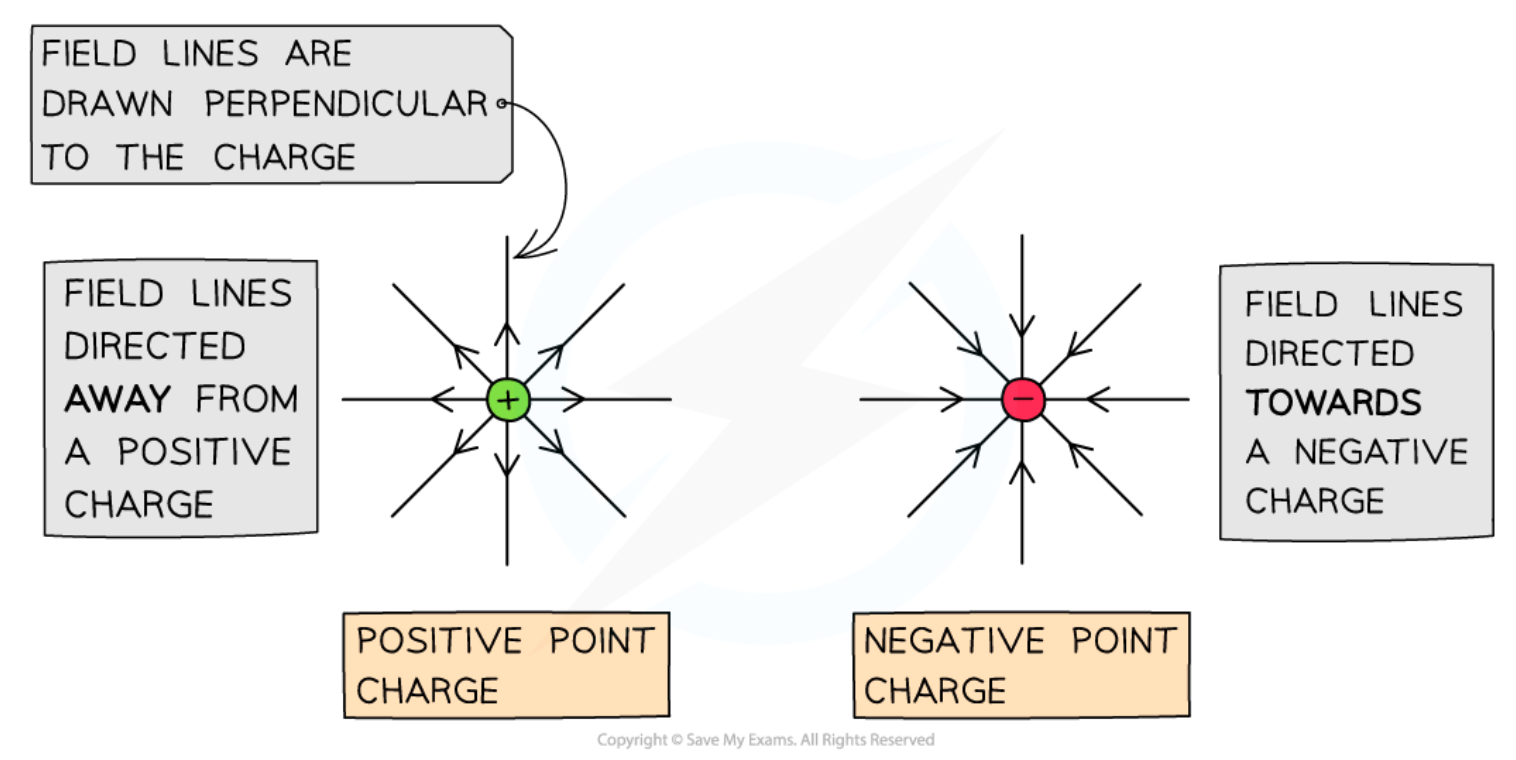
\includegraphics[width=0.5\linewidth]{截圖 2026-02-10 16.08.22.png}
\end{center}
The field lines around a charged conducting sphere are similar to that of a point charge. The charges on the surface of the sphere will be evenly distributed.
The charges are the same, so they repel. Field lines are always perpendicular (at right angles) to the surface of a conducting sphere.\\\\
\textbf{Note:} when you have questions like this: (0625/31/O/N/10) Make sure that in your explanation, ONLY the particles with the opposite charge are "being attracted", while the ones with the same charge are NOT "repelled". They just stay at the original position.
\begin{center}
    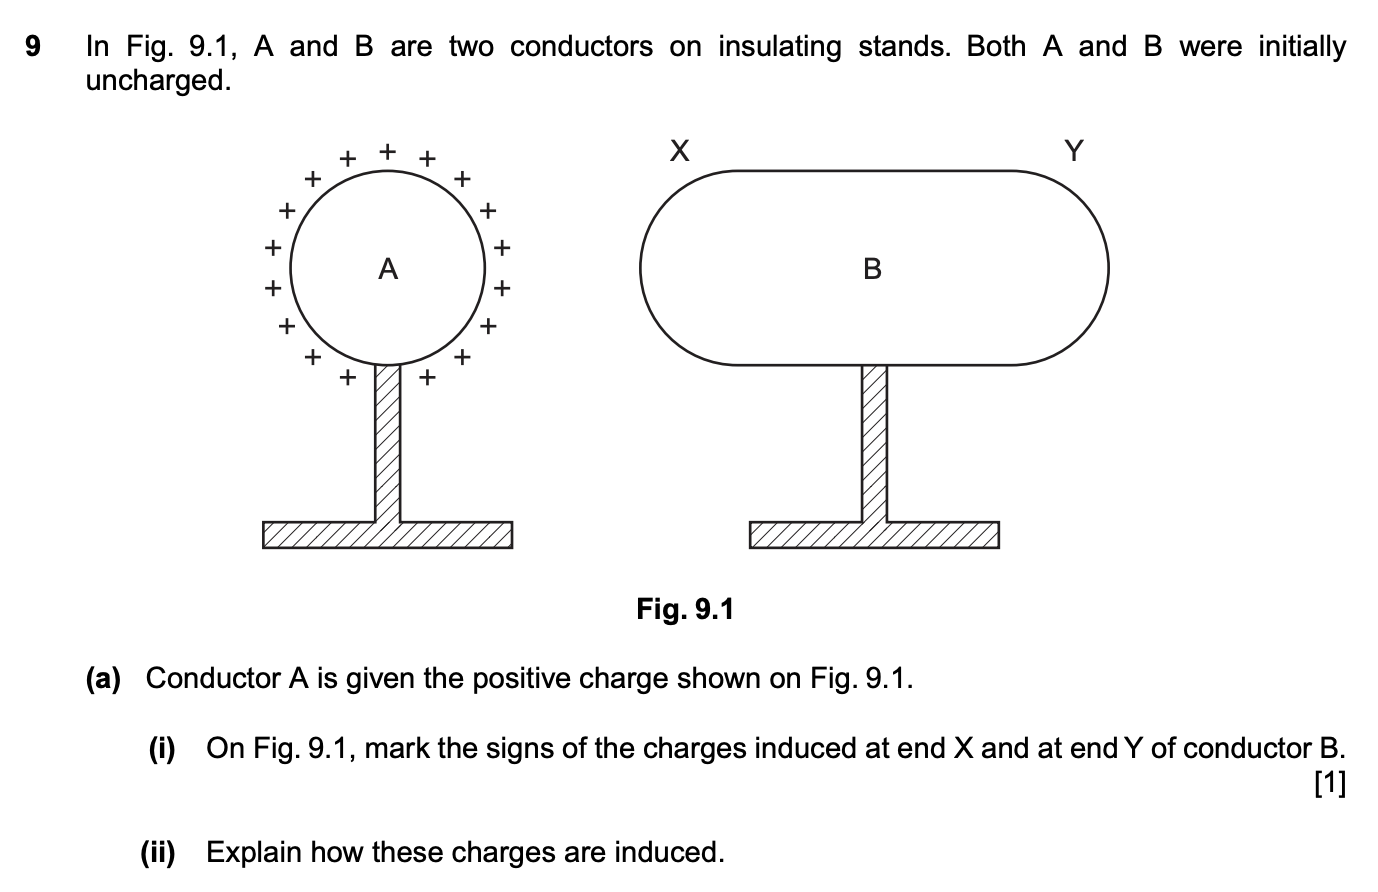
\includegraphics[width=0.7\linewidth]{屏幕快照 2026-03-11 下午10.13.26.png}
\end{center}
The electric field between two parallel plates is a uniform electric field. The field lines are:
\begin{itemize}
    \item directed from the positive to the negative plate
    \item parallel
    \item straight lines
\end{itemize}
\subsubsection{\textit{Professional} vocabs for circuits}
\begin{itemize}
    \item Current, \(I\)
    \begin{itemize}
        \item Defined as the rate of flow of electric charge
        \item In other words, \(I=\frac{Q}{t}\)
        \item Current flows from the positive terminal to the negative terminal of a cell.
        \item Ammeter must be connected in series in order to measure the current. 
        \item \textbf{Important: electron flow \& conventional current is different!} (Opposite direction)
        \item DC \& AC
        \begin{itemize}
            \item DC is defined as a steady current, constantly flowing in the same direction in a circuit, from positive to negative.
            \item AC is defined as a current that continuously changes its direction, going back and forth around a circuit.
        \end{itemize}
    \end{itemize}
    \item Electromotive Force, \(e.m.f\)
    \begin{itemize}
        \item Defined as the electrical work done by a source in moving a unit charge around a complete circuit.
        \item Ms. Lydia definition (easier to memorize): work done per unit of charge within the source
        \item \(E\ (V) = \frac{W\ (J)}{Q\ (C)}\)
    \end{itemize}
    \item Potential Difference, \(p.d.\)
    \begin{itemize}
        \item Defined as the work done by a unit charge passing through a component.
        \item Ms. Lydia definition: work done per unit of charge within the component
        \item Voltmeter must be connected in parallel in order to measure the \(p.d.\)
    \end{itemize}
    \item Resistance, \(R\ (\Omega)\)
    \begin{itemize}
        \item Defined as the opposition to current
        \item The free electrons flowing in the circuit (current) collide with the metal ions in the wire. These collisions slow down the electrons, resist their flow.
        \item Ohm's Law gives that \(R=\frac{V}{I}\)
        \item Resistance of a wire is given by \(R=\rho \frac{L}{A}\)
        \item In other words, \(R\propto L\ \&\ R\propto \frac{1}{A}\)
    \end{itemize}
    \item Electrical Energy
    \begin{itemize}
        \item Equation is \(E=VIt\)
        \item Warmly reminder: \(1\ kWh=3.6\times 10^6 J\)
        \item The amount of energy transferred by an electrical appliance depends on how long the appliance runs for \& the power rating of the appliance
    \end{itemize}
    \item Power, \(P\ (W)\)
    \begin{itemize}
        \item Defined as the rate at which energy is transferred by an appliance
        \item \(P=\frac{E}{t}=\frac{W}{t}=IV\)
    \end{itemize}
\end{itemize}
\textbf{I-V graphs for non-ohmic conductors}
\begin{center}
    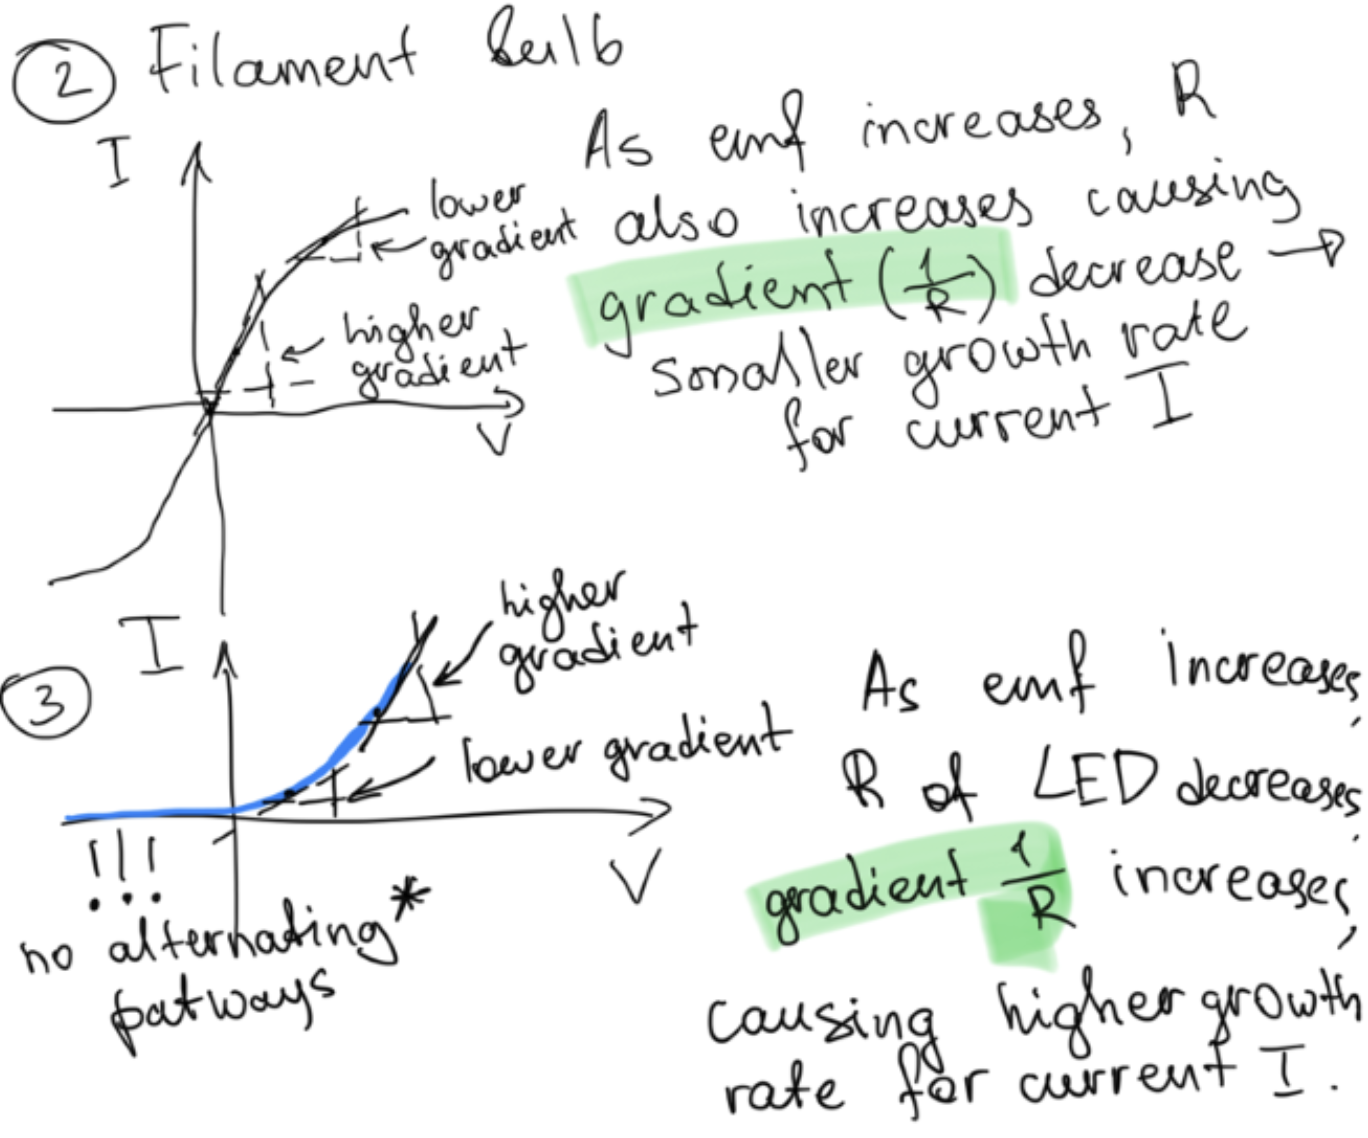
\includegraphics[width=0.45\linewidth]{屏幕快照 2026-03-11 下午10.27.48.png}
    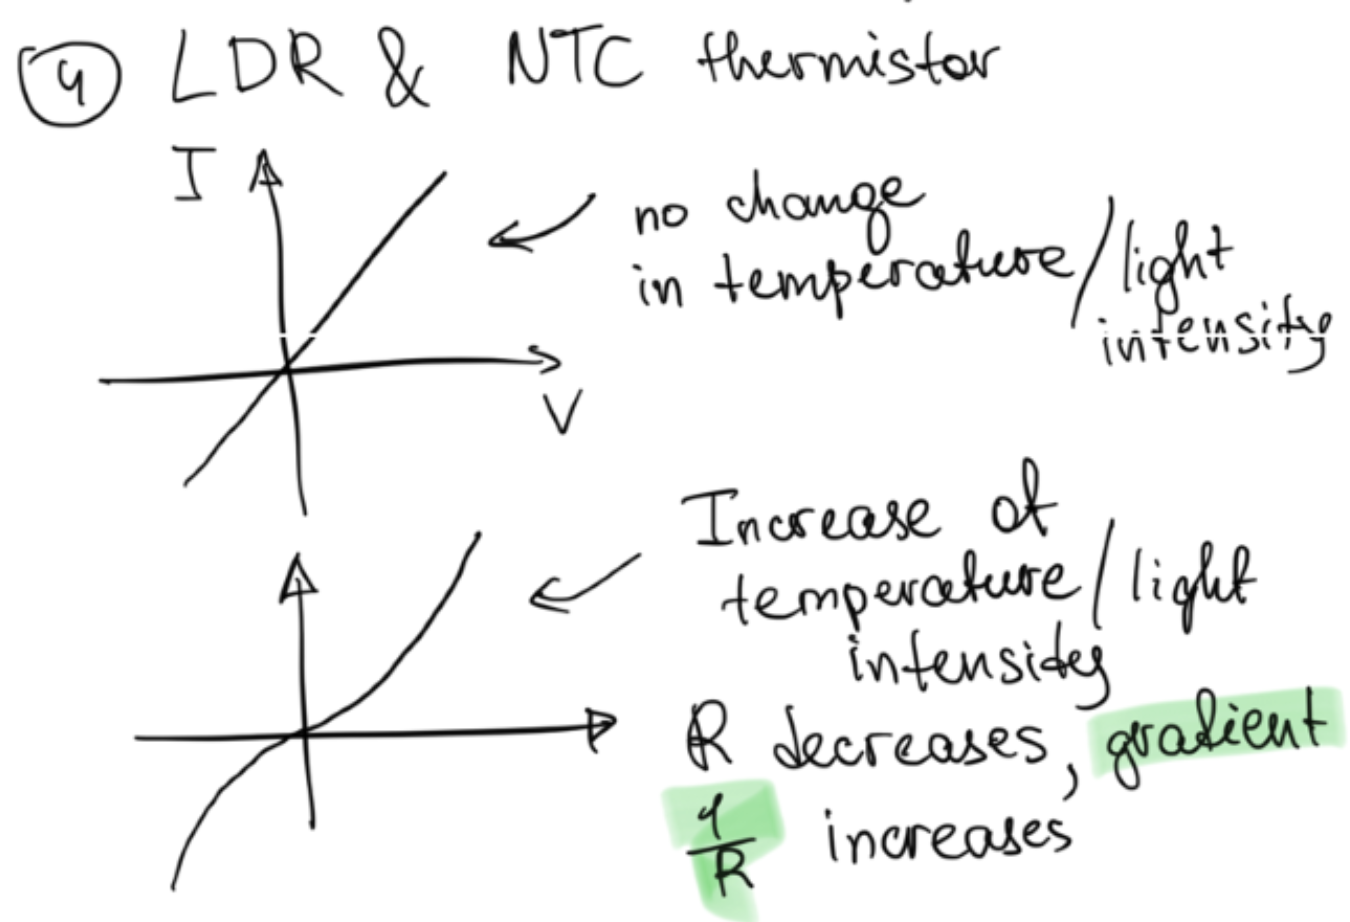
\includegraphics[width=0.5\linewidth]{屏幕快照 2026-03-11 下午10.22.52.png}
\end{center}
\newpage
\subsection{Electrical Circuit \& Safety}
Memorize this list below before we move on:
\begin{center}
    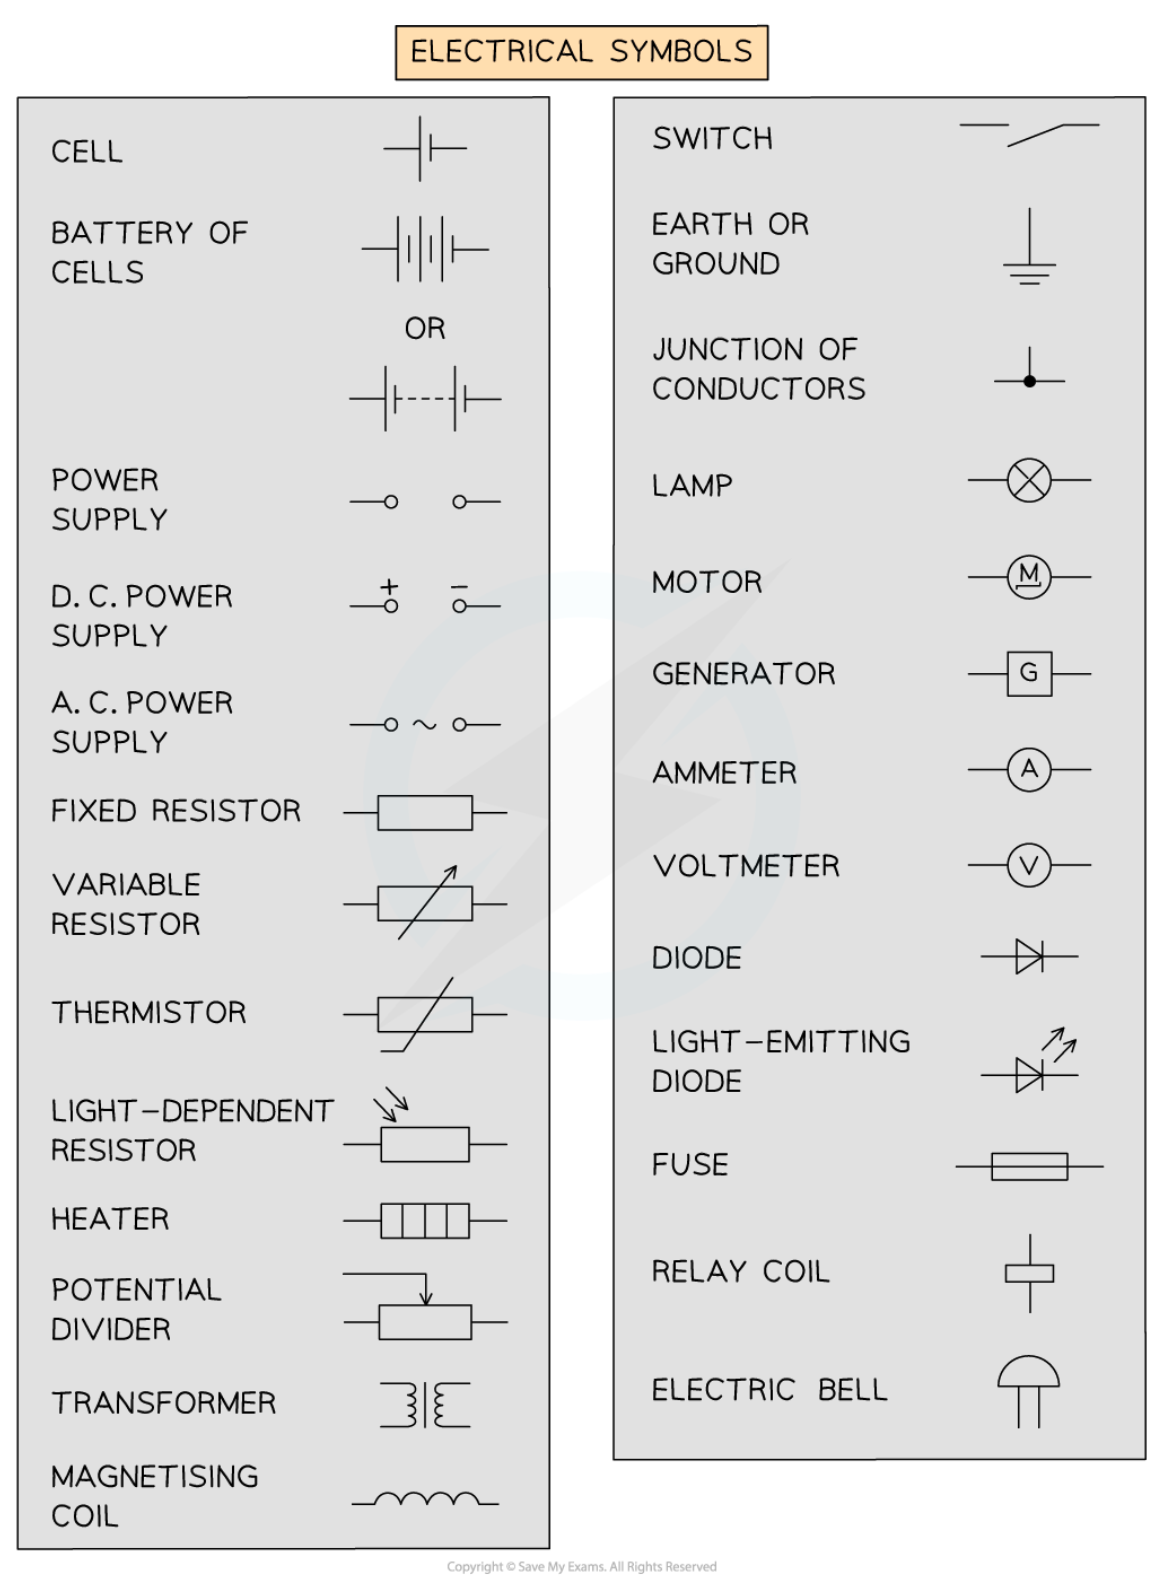
\includegraphics[width=1\linewidth]{截圖 2026-02-10 16.40.44.png}\\
    This is the worst nightmare that I've ever seen.
\end{center}
Some specific items that need a little more explanation:
\begin{itemize}
    \item Thermistors
    \begin{itemize}
        \item A thermistor is a non-ohmic conductor and a temperature-dependent resistor.
        \item As the temperature increases the resistance of a thermistor decreases and vice versa.
    \end{itemize}
    \item LDR / Light-dependent resistors
    \begin{itemize}
        \item A light-dependent resistor (LDR) is a non-ohmic conductor and sensory resistor.
        \item As the light intensity increases, the resistance of an LDR decreases.
    \end{itemize}
    \item Diodes
    \begin{itemize}
        \item Diodes only allow current to flow through them in one direction. Due to this characteristic, it is a \textbf{rectifier}.
        \\ 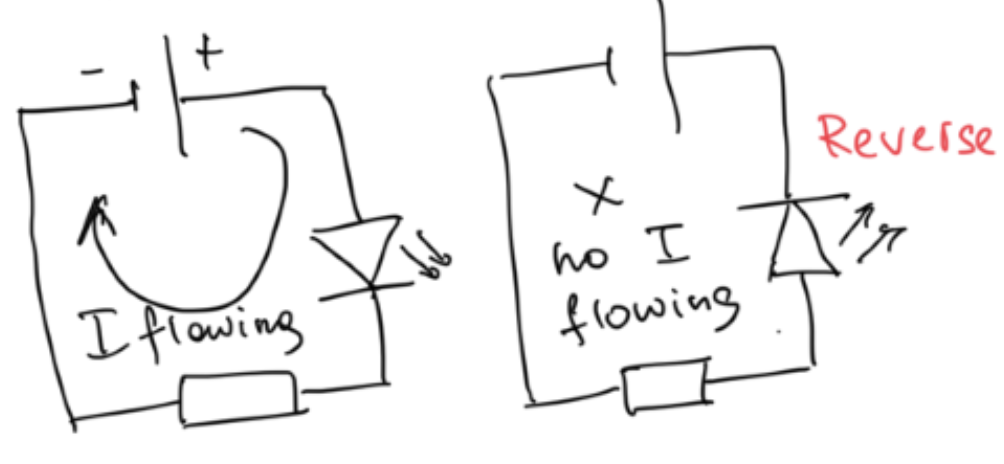
\includegraphics[width=0.5\linewidth]{屏幕快照 2026-03-11 下午10.22.28.png}
    \end{itemize}
\end{itemize}
I'm not going to explain the differences in parallel and series circuits, calculation for the total resistance, voltage, current for these two types of circuits.\\\\
\textbf{Potential Dividers}\\\\
When two resistors are connected in series, the potential difference across the power source is shared between them.\\
A potential divider is a circuit which splits potential difference from a power source, so only a fraction goes to a component.\\
The ratio of potential differences across each resistor can be found using the following equation:
\[\frac{R_1}{R_2}=\frac{V_1}{V_2}\]
\textbf{Electrical Safety}\\\\
Common Electrical Hazards:
\begin{itemize}
    \item Damaged insulation
    \item Overheating cables
    \item Damp conditions
    \item Excess current
\end{itemize}
Methods of protection:
\begin{itemize}
    \item Live, neutral, earth wires in the mains supply
    \begin{itemize}
        \item The purpose of the live wire is to carry the alternating current from the mains supply to a circuit.
        \item The purpose of the neutral wire is to form the opposite end of the circuit to the live wire to complete the circuit.
        \item The purpose of the earth wire is to act as a safety wire to stop the appliance from becoming live. This prevents electric shocks from occurring if the appliance malfunctions or the live wire breaks off and touches the case of the plug.
    \end{itemize}
    \item Double insulation
    \begin{itemize}
        \item Some appliances are said to be double insulated, as they have two layers of insulation:
        \item Insulation around the wires themselves
        \item A non-metallic case that acts as a second layer of insulation
    \end{itemize}
    \item Earthing
    \begin{itemize}
        \item The earth wire is an additional safety wire that can reduce the risk of electrical hazards.
        \item If a live wire came into contact with the case:
        \item The earth wire provides a low resistance path to the earth.
        \item It causes a surge of current in the earth wire and hence also in the live wire.
        \item The high current through the fuse causes it to melt and break.
        \item This cuts off the supply of electricity to the appliance, making it safe.
    \end{itemize}
    \item Fuses \& trip switches
    \begin{itemize}
        \item Fuses are used to protect individual appliances, and are located in the plug
        \item If the current in the wire becomes too large: the wire heats up and melts, causeing the wire to break, breaking the circuit and stopping the current
        \item The correct fuse to use is the value just above the current required for the appliance.
        \item For trip switches: when the current is too high the switch 'trips' (automatically flicks to the off position). This stops the current flowing in that circuit.
    \end{itemize}
\end{itemize}
\subsection{EM Effect}
An \(e.m.f.\) is induced in a conductor whenever there is relative movement between the conductor and a magnetic field.\\\\
\textbf{Lenz's Law}\\\\
Lenz's Law states that the direction of an induced \(e.m.f.\) always opposes the change causing it.\\
If the magnet is pushed north end first into the coil, the end of the coil closest to the magnet will become a north pole.\\
If a magnet is now pulled away from the coil of wire, the end of the coil closest to the magnet will become a south pole.
\begin{center}
    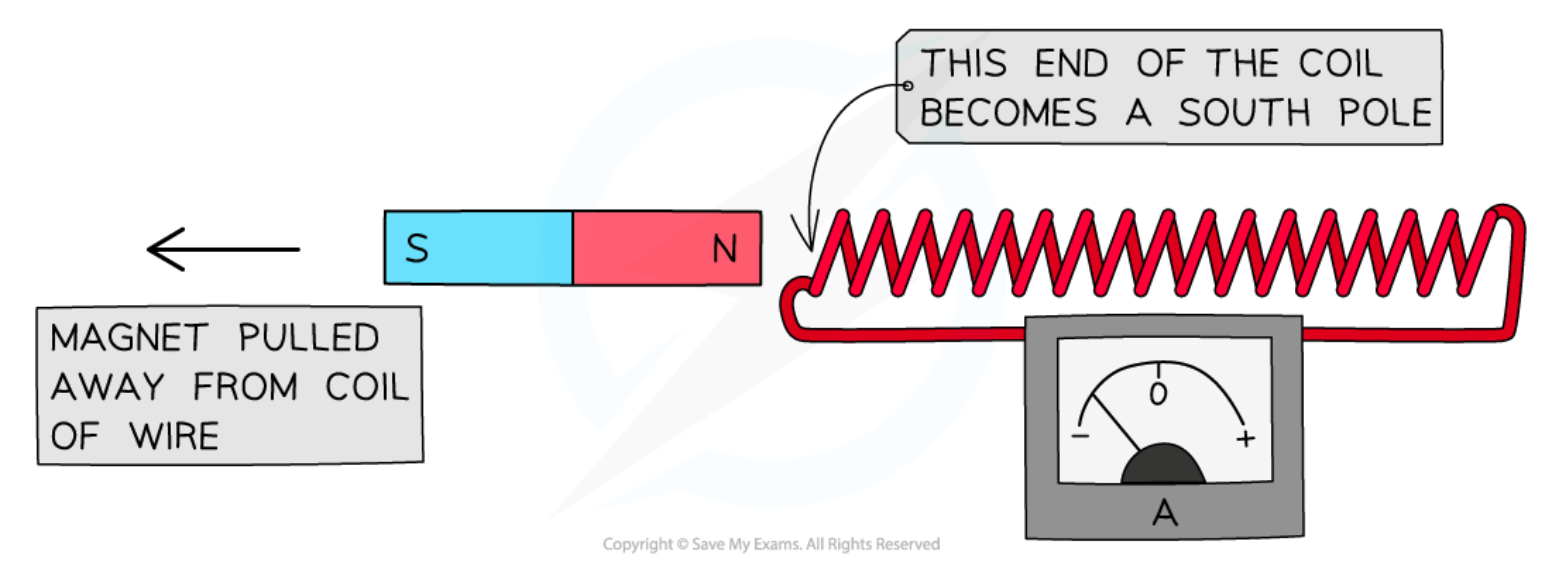
\includegraphics[width=0.55\linewidth]{截圖 2026-02-10 20.29.38.png}
\end{center}
Factors affecting the magnitude of the induced \(e.m.f.\):
\begin{itemize}
    \item The speed at which the wire, coil or magnet is moved;
    \item The number of turns on the coils in the wire;
    \item The size of the coils;
    \item The strength of the magnetic field.
\end{itemize}
Factors affecting the direction of the induced \(e.m.f.\):
\begin{itemize}
    \item The orientation of the poles of the magnet;
    \item The direction in which the wire, coil or magnet is moved.
\end{itemize}
\textbf{Relay: Annotated Diagram}
\begin{center}
    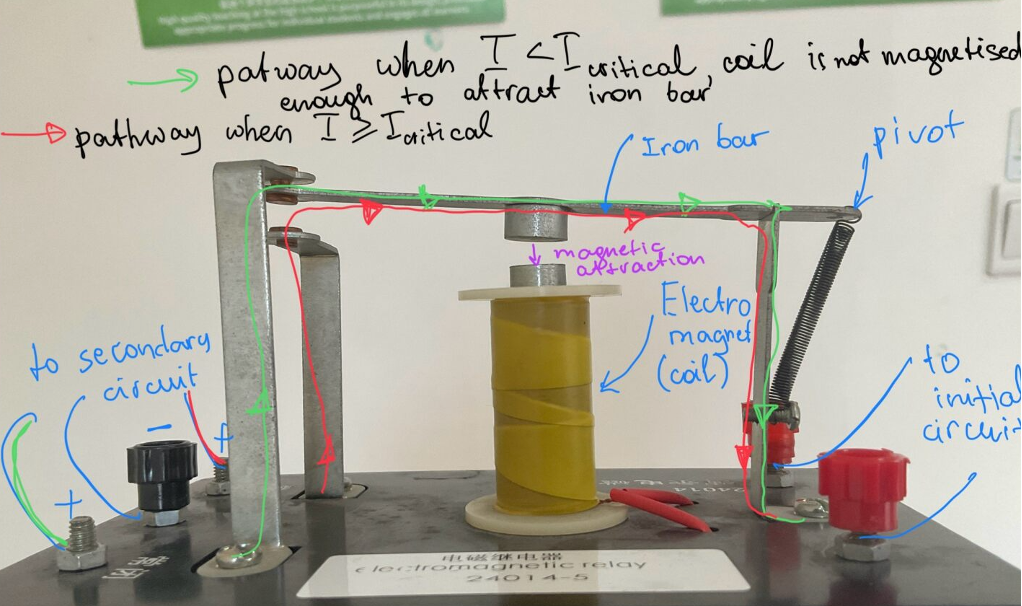
\includegraphics[width=0.9\linewidth]{图片 9.png}
\end{center}
\textbf{AC Generator}\\
\begin{center}
    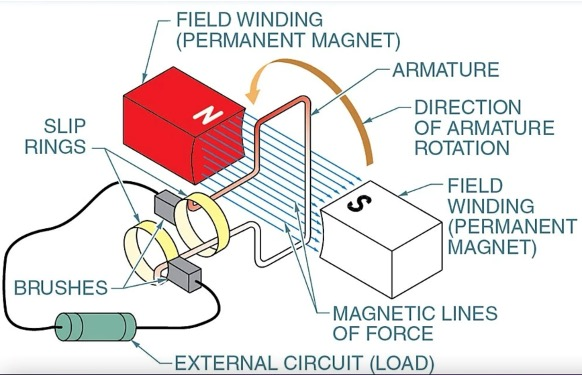
\includegraphics[width=0.6\linewidth]{圖片 1.jpg}
\end{center}
An \(e.m.f.\) is induced in the coil as it cuts the magnetic field. The pointer defects first one way, then the opposite way, and then back again. This indicates the size and direction of the \(e.m.f.\) is constantly changing.
As a result of the alternating \(e.m.f.\), an alternating current is also produced as the coil rotates.
This continues as long as the coil keeps turning in the same direction. 
\newpage
\begin{center}
\begin{tikzpicture}
    \begin{axis}[
        clip=false,
        xmin=0,
        xmax=2.5*pi,
        ymin=-1.5,
        ymax=1.5,
        axis lines=middle,
        xlabel=$time\ (s)$,
        ylabel=$e.m.f.$,
        title={Correlation between the $\sin (x)$ diagram and the changing \(e.m.f.\) produced by the AC generator}
    ]
        \addplot[domain=0:2*pi,red,samples=360]{sin(deg(x))}
        node[right,pos=0.9]{$f(x)=\sin (x)$};
    \end{axis}
\end{tikzpicture}
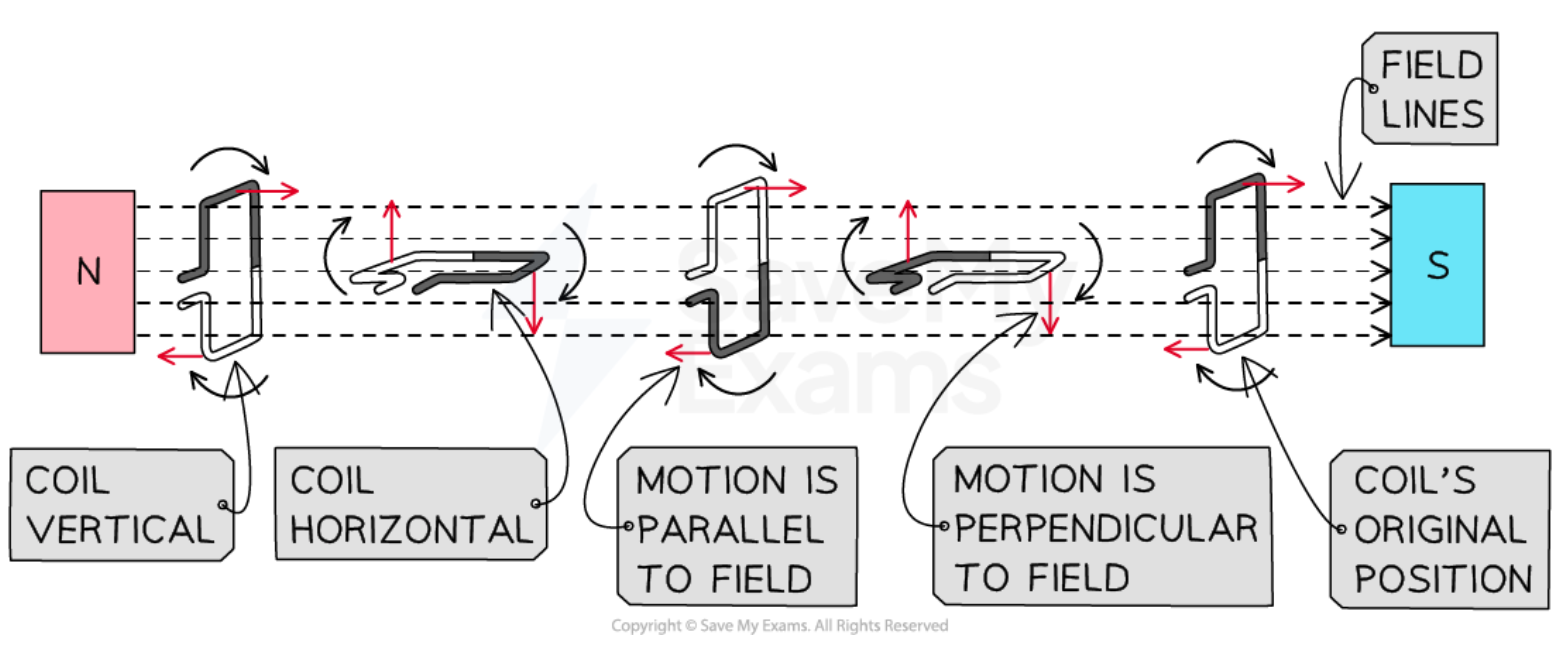
\includegraphics[width=0.7\linewidth]{截圖 2026-02-10 21.08.30.png}\\
Do you see the correlation?\\
Extension: use the following formula to deduce the magnetic flux of the magnetic field:
\[\mathcal{E}=-N\frac{d\Phi}{dt}.\ \text{I guess it's called Faraday's Law??}\]
\end{center}
The magnitude of the induced \(e.m.f.\) can be increased by:
\begin{itemize}
    \item increasing the frequency of rotation of the coil
    \item increasing the number of turns on the coil
    \item increasing the strength of the magnet
    \item inserting a soft iron core into the coil
\end{itemize}
\textbf{Magnetic Field Lines}\\
Magnetic Field around a wire can be deduced using the \textbf{right-hand grip rule.}
The magnetic field lines around a straight wire are made up of concentric circles.
\begin{center}
    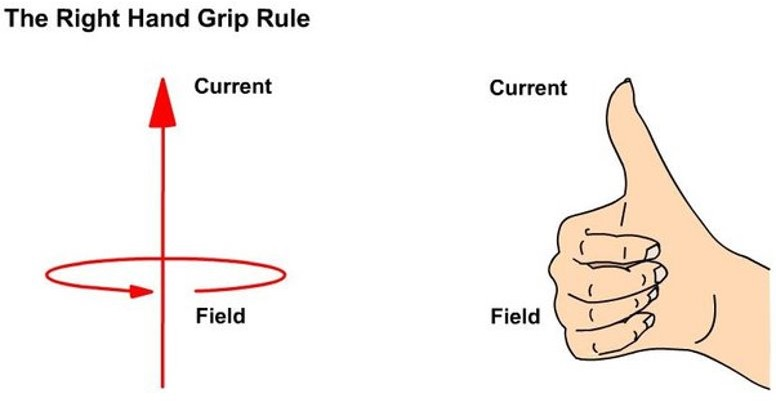
\includegraphics[width=0.5\linewidth]{圖片 2.jpg}
\end{center}
As seen from a current-carrying wire, an electric current produces a magnetic field.\\
An electromagnet utilises this by using a coil of wire called a solenoid.\\
This increases the strength of the magnetic field by adding more turns of wire into a smaller region of space. 
One end of the solenoid becomes a north pole, and the other becomes the south pole.\\
\begin{center}
    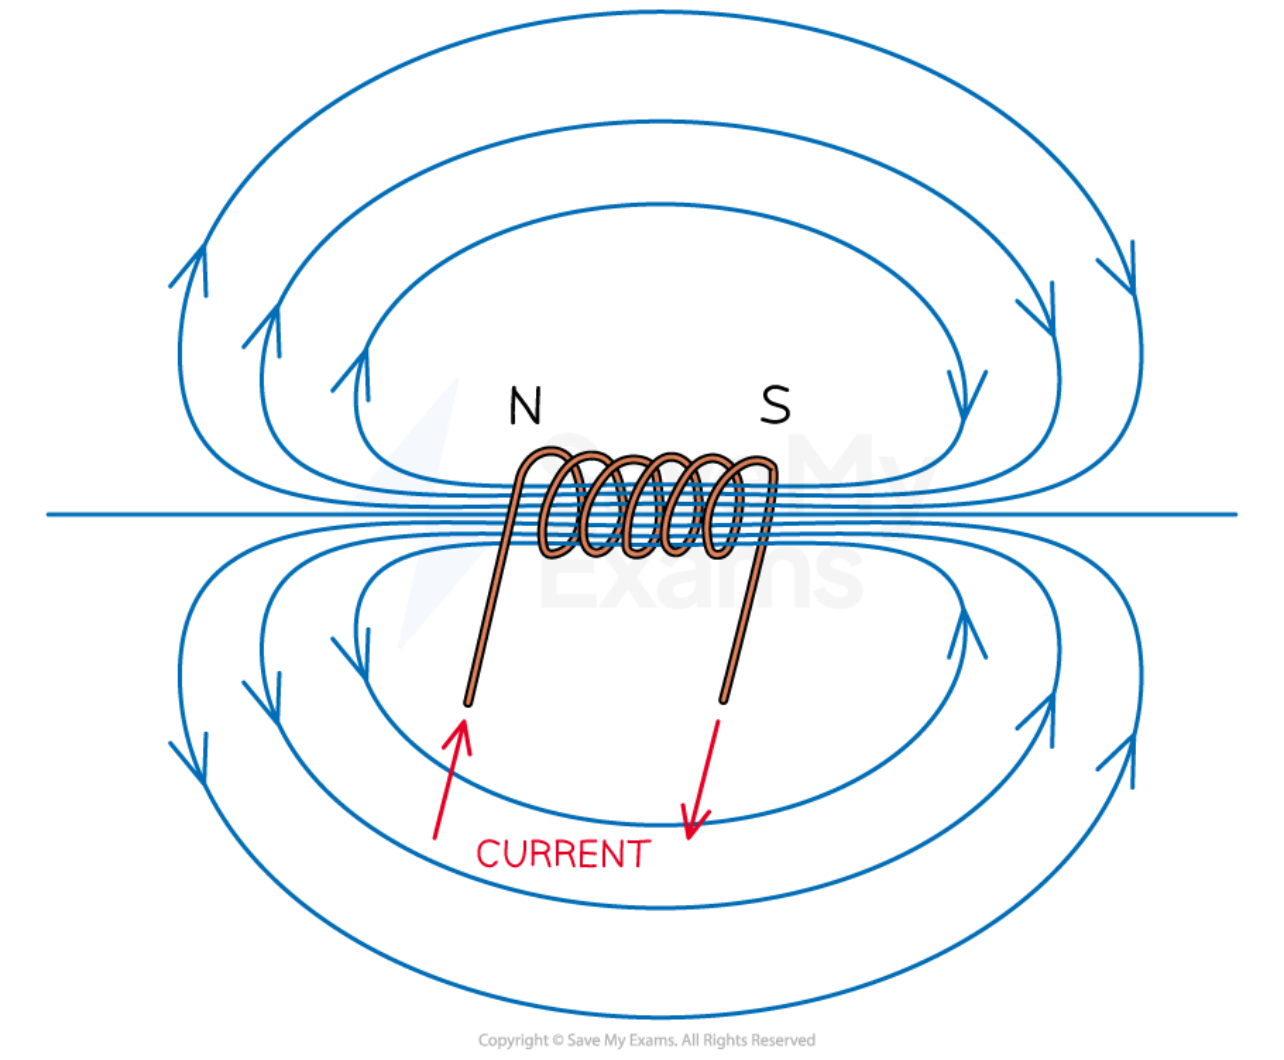
\includegraphics[width=0.5\linewidth]{截圖 2026-02-10 21.44.43.png}
    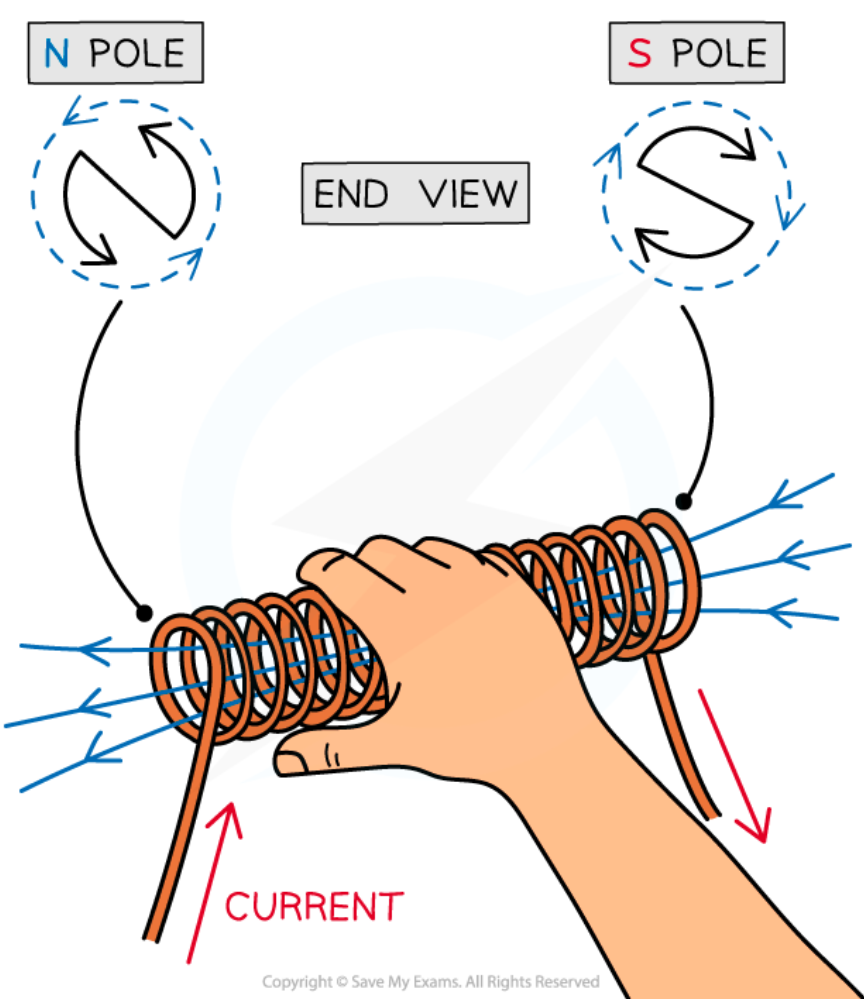
\includegraphics[width=0.4\linewidth]{截圖 2026-02-10 21.44.54.png}
\end{center}
A circular coil is equivalent to one of the coils of a solenoid. The field lines emerge through one side of the circle (north pole) and enter through the other (south pole).
\begin{center}
    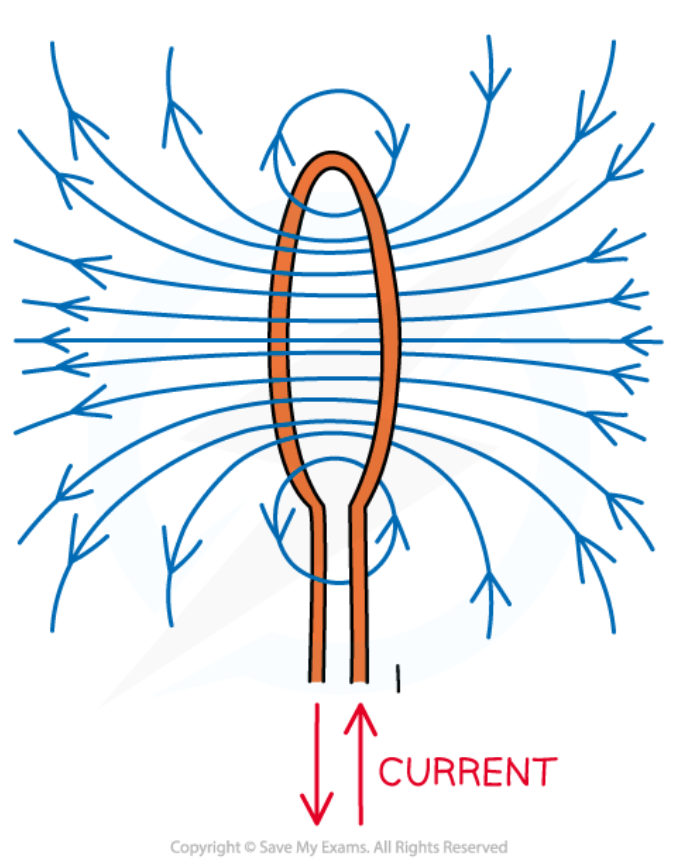
\includegraphics[width=0.5\linewidth]{截圖 2026-02-10 21.45.09.png}
\end{center}
The strength of the magnetic field around a wire depends on \textbf{the size of the current \& the distance from the wire.} When the direction of the current changes, the magnetic field acts in the opposite direction.\\
The strength of the magnetic field produced around a solenoid can be increased by:
\begin{itemize}
    \item increasing the amount of current flowing through the coil
    \item increasing the number of turns on the coil
    \item inserting an iron core into the coil
\end{itemize}
The magnetic effect of a current can be used in relay circuits and loudspeakers.\\\\
\textbf{Relay circuits (electric bells)}\\\\
Electromagnets are commonly used in relay circuits.
\begin{center}
    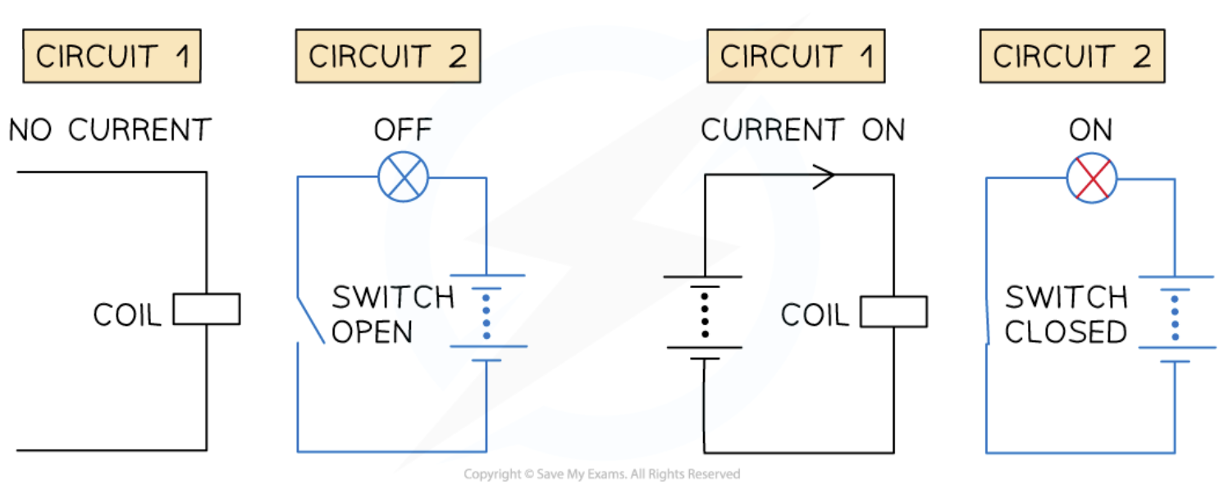
\includegraphics[width=0.8\linewidth]{圖片 3.png}
\end{center}
When a current flows through Circuit 1, a magnetic field is induced around the coil. 
The magnetic field attracts the switch, causing it to pivot and close the contacts in Circuit 2.
This allows a current to flow in Circuit 2.\\\\
Electric bells utilise relay circuits. As the current alternates, the metal arm strikes the bell and drops repeatedly to produce the ringing effect.\\\\
\textbf{Loudspeakers}\\\\
Loudspeakers convert electrical signals into sound waves. They work due to the motor effect.\\
\begin{center}
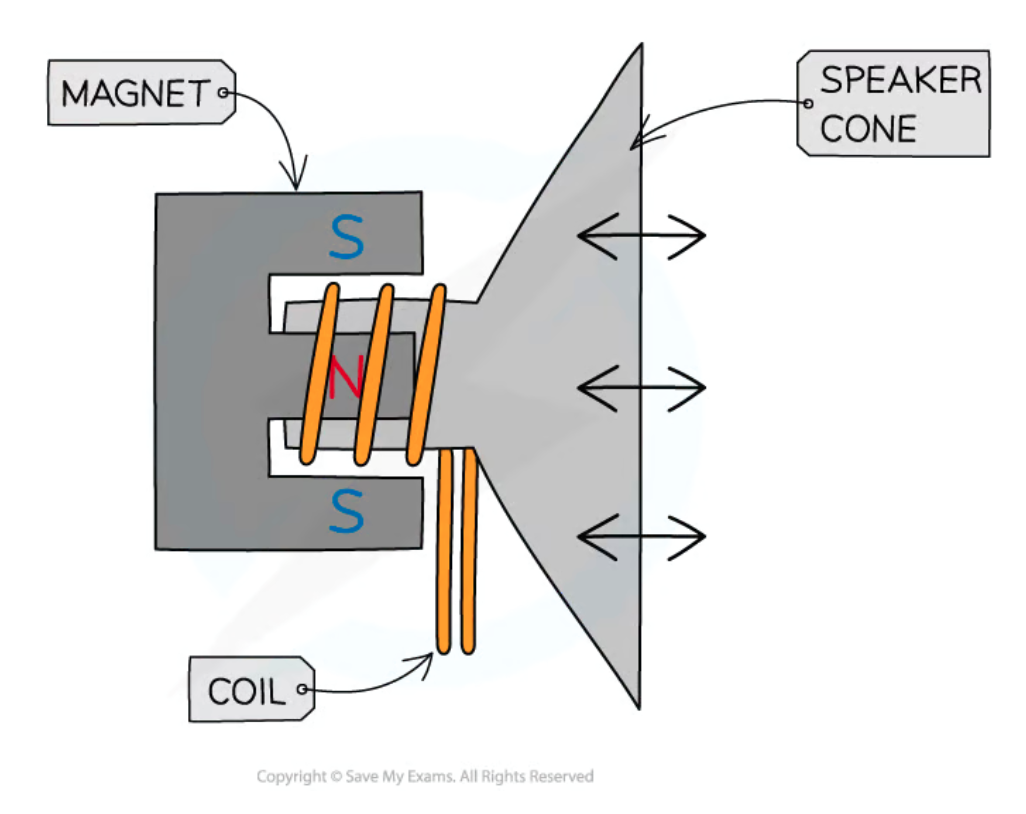
\includegraphics[width=0.6\linewidth]{截圖 2026-02-10 22.00.05.png}
\end{center}
An alternating current passes through the coil of the loudspeaker, which creates a changing magnetic field around the coil. 
As the current is constantly changing direction, the direction of the magnetic field will be constantly changing.
The magnetic field produced around the coil interacts with the field from the permanent magnet.
The interacting magnetic fields will exert a force on the coil. \\
As the magnetic field is constantly changing direction, the force exerted on the coil will constantly change direction.
This makes the coil oscillate, causing the speaker cone to oscillate, making the air oscillate, creating sound waves.\\\\
\textbf{\(F\) on current-carrying conductor}\\\\
A current-carrying conductor produces its own magnetic field. When interacting with an external magnetic field, it will experience a force.
A current-carrying conductor will only experience a force if the current through it is perpendicular to the direction of the magnetic field lines.\\
Two ways to reverse the direction of the force are by reversing the direction of the current / the magnetic field.\\\\
\textbf{Flemming Left Hand Rule \& Right Hand Rule (Use any rule you found comfortable)}\\
\begin{tikzpicture}[x=0.5cm,y=0.5cm,z=0.3cm,>=stealth]
\draw[->] (xyz cs:x=0) -- (xyz cs:x=13.5) node[above] {$Current\ (I)$};
\draw[->] (xyz cs:y=0) -- (xyz cs:y=13.5) node[right] {$Force\ (F)$};
\draw[->] (xyz cs:z=0) -- (xyz cs:z=13.5) node[above] {$Magnetic\ Field\ (B)\ N\ to\ S$};
\end{tikzpicture}
\begin{tikzpicture}[x=0.5cm,y=0.5cm,z=0.3cm,>=stealth]
\draw[<-] (xyz cs:x=-13.5) -- (xyz cs:x=0) node[left,above] {$Magnetic\ Field\ (B)$};
\draw[->] (xyz cs:y=0) -- (xyz cs:y=13.5) node[right] {$Direction\ of\ Motion$};
\draw[->] (xyz cs:z=0) -- (xyz cs:z=-13.5) node[above] {$Current\ (I)$};
\end{tikzpicture}\\
\begin{center}
    
\includegraphics[width=0.32\linewidth]{109951166485403477.jpg}
\end{center}
When a current-carrying wire is placed in a magnetic field, it will experience a force if the wire is perpendicular.
This is because the magnetic field exerts a force on each individual electron flowing through the wire.
Therefore, when a charged particle passes through a magnetic field, the field can exert a force on the particle, causing it to deflect.
The force is always at 90 degrees to both the direction of travel and the magnetic field lines. \textbf{Use Left Hand Rule for deducing direction of deflection of (+) particles \& use Right Hand Rule for deducing direction of deflection of (-) particles.}
\begin{center}
    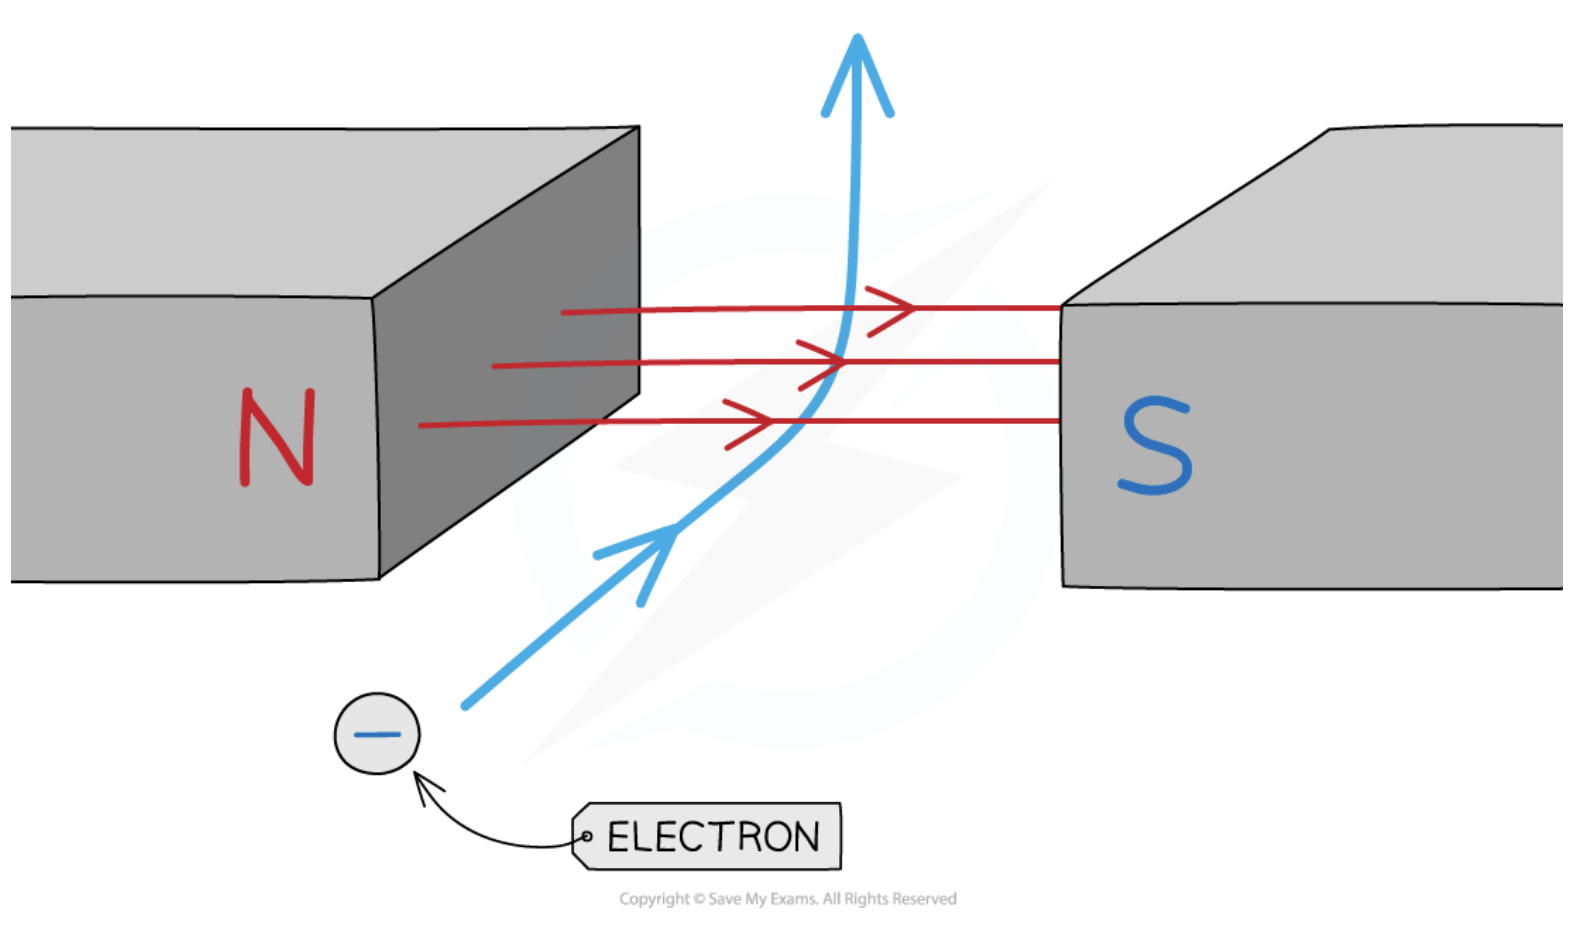
\includegraphics[width=0.6\linewidth]{截圖 2026-02-11 16.26.44.png}
\end{center}
\textbf{DC Motor}
\begin{center}
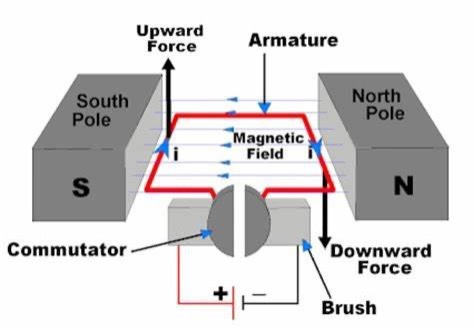
\includegraphics[width=0.6\linewidth]{圖片 3.jpg}
\end{center}
A DC motor consists of a coil of wire between the poles of a permanent magnet, a \textbf{(split-ring) commutator} and brushes connected to a DC source.
The brushes and commutator are designed to reverse current every half turn, so that the coil can keep spinning without changing direction of rotation.\\
\textbf{Just remember the word commutator or else you would be very confused. \\(Slip rings vs Split-ring commutator)}\\
The turning effect of the coil can be increased by increasing the number of turns on the coil, the current of the coil, the strength of the magnetic field.\\
The speed of rotation can be increased by increasing the current \& using a stronger magnet.\\
The direction of rotation of the coil in the DC motor can be changed by reversing the direction of the current supply or by swapping the poles of the magnet.\\
The force supplied by the motor can be increased by increasing the current flowing through the coil, increasing the strength of the magnetic field, or increasing the number of turns on the coil.\\\\
\textbf{Transformer}\\\\
A transformer is a device used to change the size of an alternating voltage or current. \\Iron is used because it is easily magnetized.\\
\begin{center}
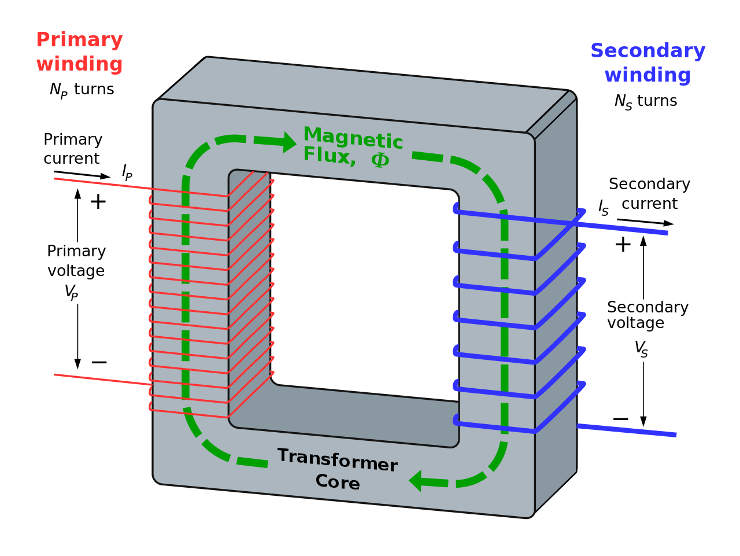
\includegraphics[width=0.5\linewidth]{截圖 2026-02-11 16.43.42.png}
\end{center}
A transformer consists of two coils of wire wound around an iron core. The primary coil is connected to the alternating current supply, and the secondary coil is connected to the load.\\\\
For a \textbf{step-up transformer}:
\begin{itemize}
    \item The primary coil has fewer turns than the secondary coil, \(N_p<N_s\)
    \item The voltage is increased, \(V_p<V_s\), less current, less energy loss.
\end{itemize}
For a \textbf{step-down transformer}:
\begin{itemize}
    \item The primary coil has more turns than the secondary coil, \(N_p>N_s\)
    \item The voltage is decreased, \(V_p>V_s\), more current, more energy loss.
\end{itemize}
Operation of a transformer:
\begin{enumerate}
    \item An alternating current in the primary coil produces a changing magnetic field around the coil.
    \item The iron core is easily magnetised, so the changing magnetic field passes through it.
    \item This changing field cuts through the secondary coil and induces an \(e.m.f\).
    \item The alternating \(e.m.f.\) will have the same frequency as the alternating current supplied to the primary coil;
    \item The induced \(e.m.f\) causes a current to flow in the secondary coil.
\end{enumerate}
The transformer equation states that the ratio of the voltages across the primary and secondary coils of a transformer is equal to the ratio of the number of turns on each coil. Equation:
\[\frac{V_p}{V_s}=\frac{N_p}{N_s};\ V_s=V_p \times \frac{N_s}{N_p}\]
Ideal transformers are 100\% efficient, under this circumstance:
\[\text{Power in primary coil = Power in secondary coil}\]
\[P_p=P_s;\ I_pV_p=I_sV_s;\ \frac{I_s}{I_p}=\frac{V_p}{V_s}\]
The power dissipated in the wire due to resistance is given by \(P=I^2R\).
\newpage
\section{Nuclear Physics}
Atoms are the building blocks of all matter.
They consist of a small dense positively charged nucleus and negatively charged electrons in orbit around the nucleus.
I'm not going to state what are isotopes, atoms, ions, atomic number, proton number, mass and relative charge of electrons, protons, neutrons, because we all learned this in chemistry. (Once again)
\subsection{Nuclear Model}
\textbf{Rutherford's \(\alpha\) scattering experiment (a.k.a. Rutherford had gold chain)}\\
In Rutherford's \(\alpha\) scattering experiment, the scattering of \(\alpha\) particles by a sheet of thin metal supports the nuclear model of the atom. It proves that:
\begin{itemize}
    \item there is a very small nucleus surrounded by mostly empty space: Most of the \(\alpha\) particles passed straight through the foil.
    \item the nucleus is containing most of the mass of the atom: A few of the \(\alpha\) particles bounced back off.
    \item a nucleus that is positively charged: Some of the \(\alpha\) particles were deflected.
\end{itemize}
\begin{center}
    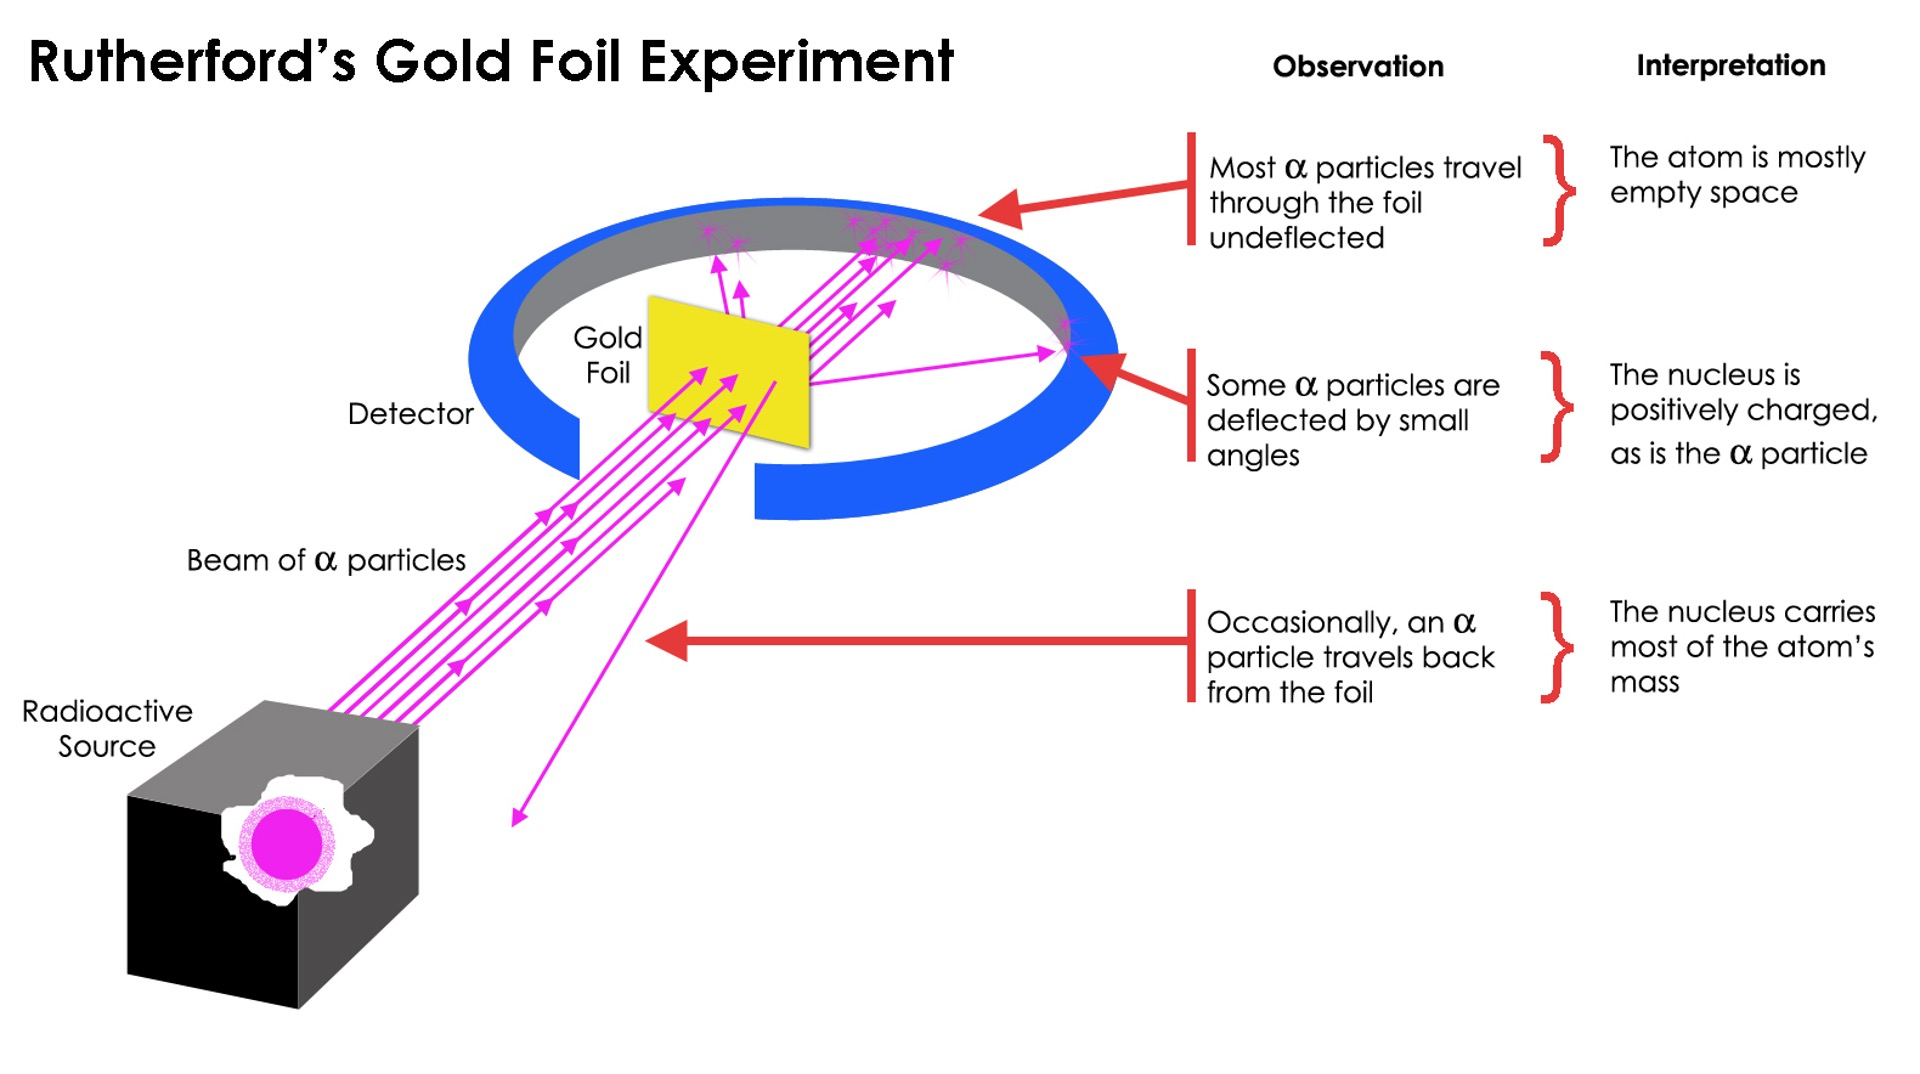
\includegraphics[width=1\linewidth]{圖片 4.jpg}
\end{center}
Nuclear fission \& fusion are nuclear reactions that change the nucleus of an atom to produce high amounts of energy from the energy stored in the nucleus of an atom. Overall, energy is conserved.\\\\
\textbf{Nuclear fission is defined as:}
\begin{center}
    \textbf{The splitting of a large, unstable nucleus into two smaller nuclei.}
\end{center}
A neutron collides with an unstable nucleus, and the nucleus splits into two smaller nuclei / daughter nuclei and 2/3 neutrons. \\\\
\textbf{Nuclear fusion is defined as:}
\begin{center}
    \textbf{When two light nuclei join to form a heavier nucleus.}
\end{center}
Stars use nuclear fusion to produce energy. Nuclear fusion requires extremely high temperature and pressure, so fusion is very hard to reproduce on Earth.
\subsection{Radioactivity}
\subsubsection{Background Radiation: the radiation that exists around us all the time}
Two types of background radiation: natural \& man-made sources.\\
Sources of background radiation include radon gases, rocks \& buildings, food \& drink, cosmic rays, \(C-14\), medical sources, nuclear waste, nuclear fallout from nuclear weapons, nuclear accidents like \textbf{CHERNOBYL}.\\\\
Ionising nuclear radiation can be measured using a detector connected to a counter. The detector uses count rate measured in counts/s, meaning number of decays/s. \\
The count rate decreases the further the detector is from the source.\\\\
\textbf{Half-life graph reading notice:} measurements of background radiation are used to determine a corrected count rate. \\\\
Some atomic nuclei are unstable. This is because of an imbalance in the forces within the nucleus. Instability is commonly due to the nucleus having too many protons or neutrons / the nucleus being very large. Unstable nuclei can emit radiation to become more stable. Radiation can be in the form of a high-energy particle or wave.\\\\
\textbf{Types of radiation: \(\alpha,\ \beta,\ \gamma\)}
\begin{center}
    \begin{tabular}{|>{\centering\arraybackslash}p{0.15\linewidth}|>{\centering\arraybackslash}p{0.25\linewidth}|>{\centering\arraybackslash}p{0.25\linewidth}|>{\centering\arraybackslash}p{0.25\linewidth}|}\hline
        Type & \(\alpha\) particle& \(\beta\) particle& \(\gamma\) ray\\\hline
        What is it? & \(He\) nuclei & Electron & EM wave with high \(f\) \\\hline
        Charge & +2 & -1 & N/A \\\hline
        Relative Mass & 4 & 0 & 0 \\\hline
        Change in element? & Yes & Yes & No \\\hline
        Ionizing power & Very high & Average & No \\\hline
        Penetrating power & Stop by paper & Stop by 5mm \(Al\) foil & Stop by 5cm lead \\\hline
        Applications & Smoke detector & Thickness of paper / foil control & Medicine \\ \hline
        Equations (Details) & \(_Z^AX \to _{Z-2}^{A-4}Y+_2^4\alpha\) & \(_Z^AX \to _{Z+1}^{A}Y+_{-1}^0\beta\) & \(_Z^AX \to _{Z}^{A}X+_{0}^0\gamma\)\\ \hline
    \end{tabular}
\end{center}
Nuclear radiation can ionise the atoms that it hits: this is mostly done by removing an electron so the atom loses a negative charge and is left with an overall positive charge.
\subsubsection{Deflection in electric fields}
\begin{center}
    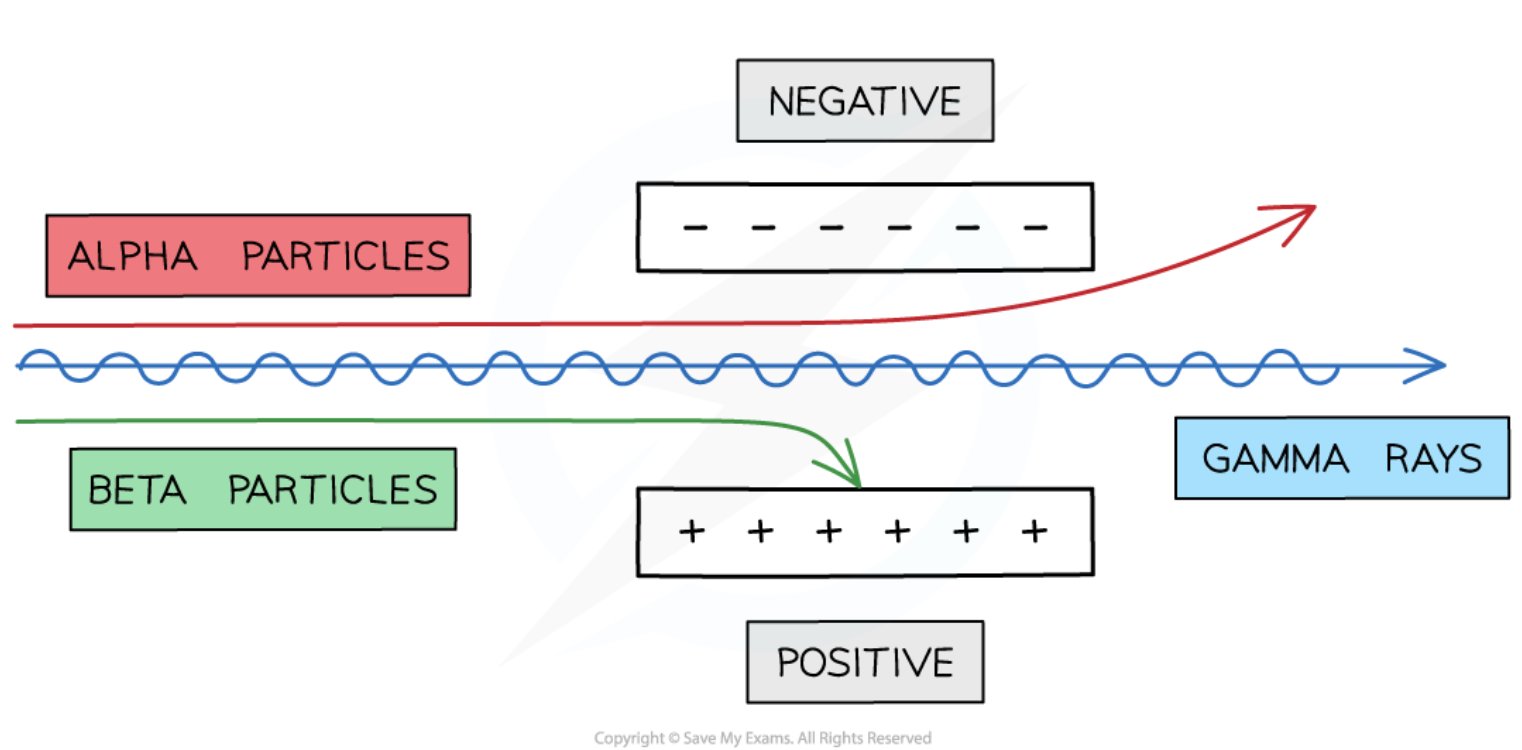
\includegraphics[width=0.6\linewidth]{截圖 2026-02-11 21.30.14.png}
\end{center}
Similarly, \(\alpha\) and \(\beta\) particles are deflected by magnetic fields whilst they are moving. They are deflected in opposite directions due to their opposite charges.
\subsubsection{Half-life (not the game developed by Valve)}
\textbf{The half-life of a radioactive isotope is the time taken for half the nuclei of that isotope in any sample to decay.} \\
The rate at which the activity of a sample decreases is measured in terms of half-life.\\
Different isotopes have different half-lives and half-lives can vary from a fraction of a second to billions of years in length.
The half-life is constant for a particular isotope.\\
\begin{center}
    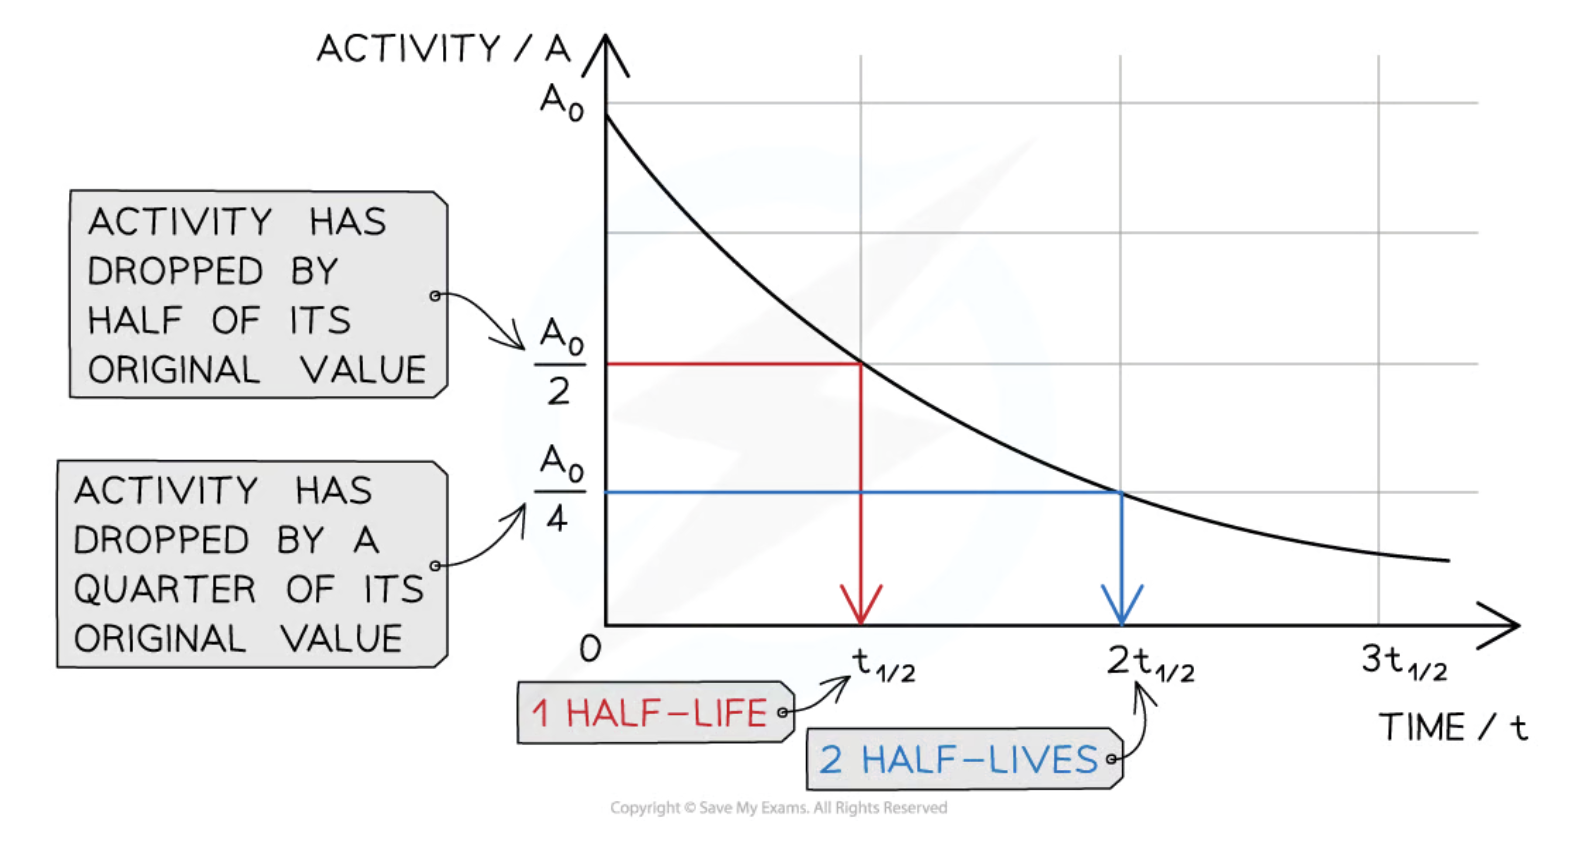
\includegraphics[width=0.8\linewidth]{截圖 2026-02-11 22.25.30.png}
\end{center}
Proportion of isotope remaining can be calculated using \(\frac{1}{2^n}\), 
where \(n\) is the number of half-lives.\\
\textbf{Remember: decay is random! You don't get the same number of decay every time you measure.}
\subsubsection{Applications}
\begin{itemize}
    \item Household fire (smoke) alarms -- \(\alpha\)
    \begin{itemize}
        \item The \(\alpha\) radiation ionises the air within the detector, creating a current;
        \item The \(\alpha\) emitter is blocked when smoke enters the detector.
        \item The alarm is triggered by a microchip when the sensor no longer detects the \(\alpha\) particles.
        \item An isotope of \(\alpha\) radiation with a long half-life is used for smoke detectors so they don't need replacing often.
    \end{itemize}
    \item Irradiating food to kill bacteria - \(\gamma\)
    \begin{itemize}
        \item It is penetrating enough to irradiate all sides of the instruments.
    \end{itemize}
    \item Sterilisation of equipment using \(\gamma\) rays
    \item Measuring and controlling thicknesses of materials -- \(\beta\)
    \begin{itemize}
        \item \(\alpha\) particles are used for thinner materials because they have a lower penetrating power and are absorbed by a thin sheet of aluminium.
        \item \(\gamma\) radiation can be used for very thick materials because they have a higher penetrating power and are mostly absorbed by thick pieces of lead.
    \end{itemize}
    \item Diagnosis and treatment of cancer using \(\gamma\) rays
    \begin{itemize}
        \item Radiotherapy is the name given to the treatment of cancer using radiation;
        \item \(\gamma\) rays are used because they can penetrate the body, reaching the tumour.
    \end{itemize}
\end{itemize}
\subsubsection{Radiation Hazards}
\begin{itemize}
    \item Cell death
    \item Mutations
    \item Cancer
    \item Skin burns
    \item Radiation sickness
\end{itemize}
\subsubsection{Safe storage}
\begin{itemize}
    \item Store the sources in lead-lined boxes and keep them at a distance from people;
    \item Minimise the amount of time you handle sources and return them to their boxes as soon as you have finished using them;
    \item During use, keep yourself (and others) as far from the sources as possible;
    \item When handling the sources do so at the length of your arms, using a pair of tongs;
    \item Reduce exposure time, increase the distance between the source and living tissue, \& use shielding to absorb radiation;
    \item Safe transportation to minimise the dangers of radioactivity;
    \item Disposing of radioactive waste (buried underground in lead-lined containers, or stored in a secure place) to minimise the dangers of radioactivity.
\end{itemize}
\begin{center}
    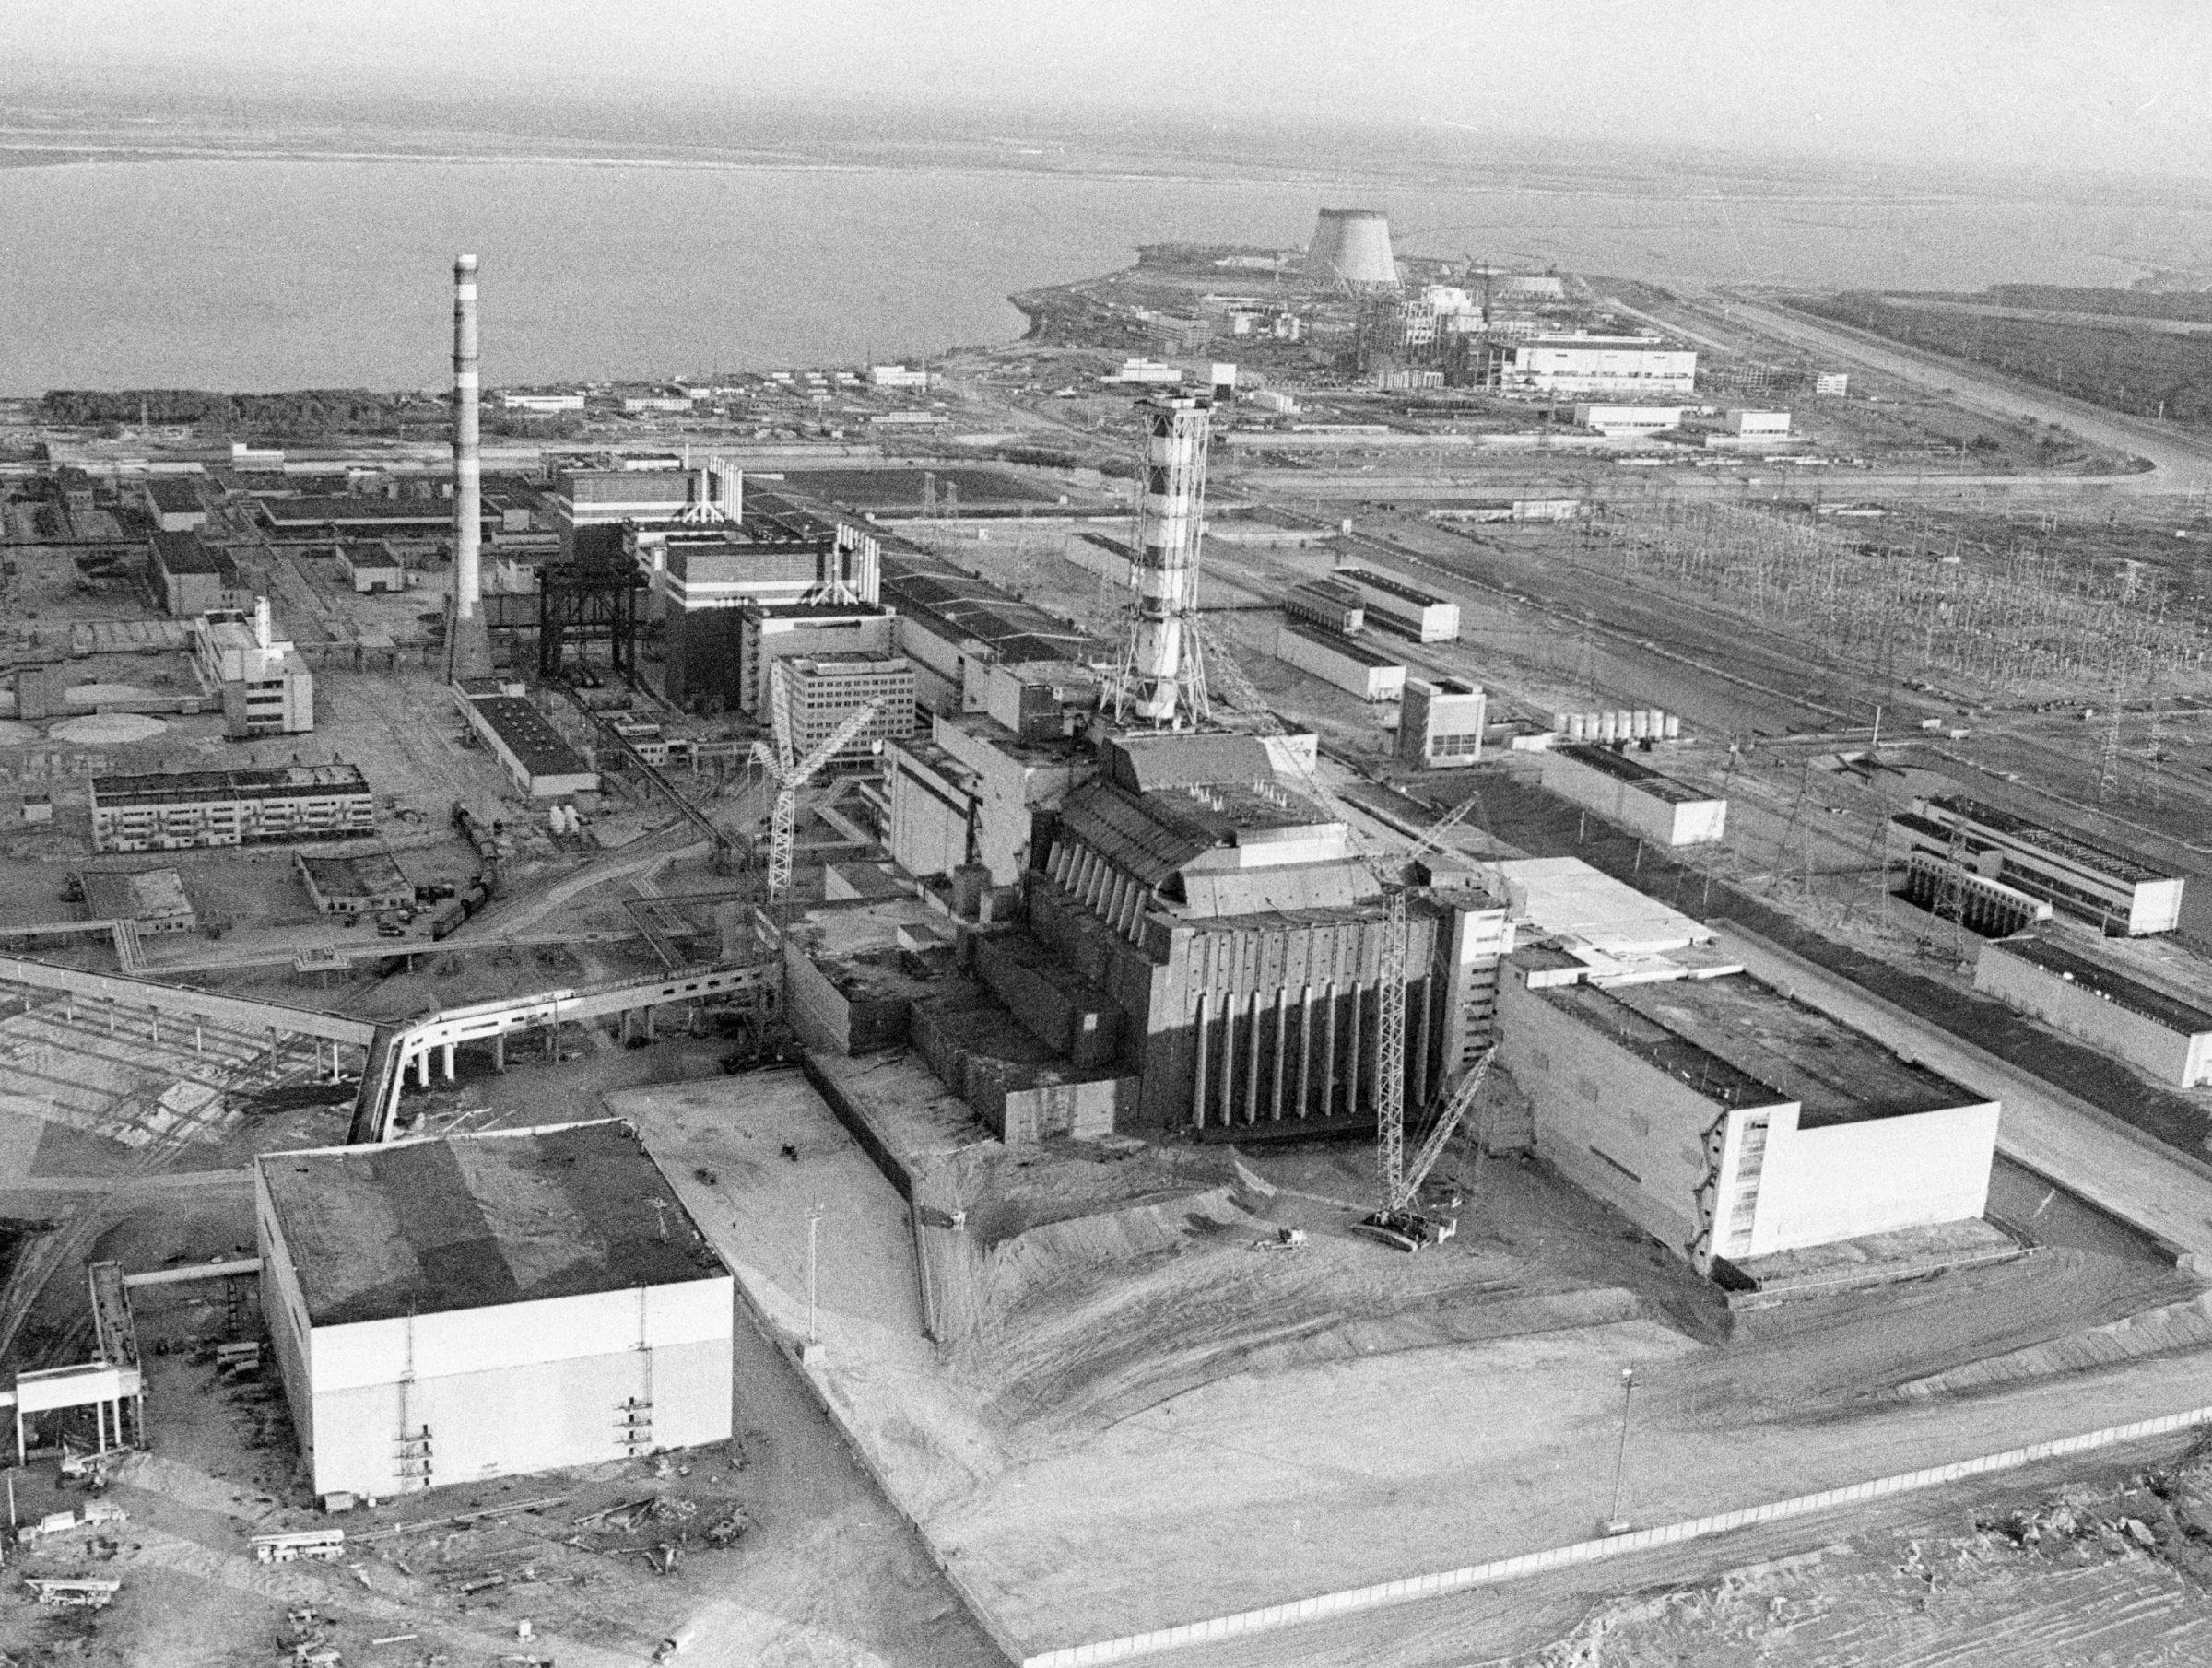
\includegraphics[width=0.9\linewidth]{B9CBW7__Chernobyl_nuclear_power_plant-2400x1810.jpg}\\
    We don't want this to happen again. A picture of the Chernobyl Nuclear Power Plant.
\end{center}
\newpage
\section{Space}
\subsection{Our home \& the Solar System}
The Earth is a planet that rotates on its axis once every 24 hours, orbits around the Sun once every 365 days. The Earth's axis is a line that passes through the North and South poles \& tilted at an angle of approximately \(23.5\degree \) from the vertical.\\
Sun appears to rise from the East \& set in the West (just in case).\\
There are differences in the amount of solar radiation that we receive. \\That's why there are different seasons. 
\begin{center}
    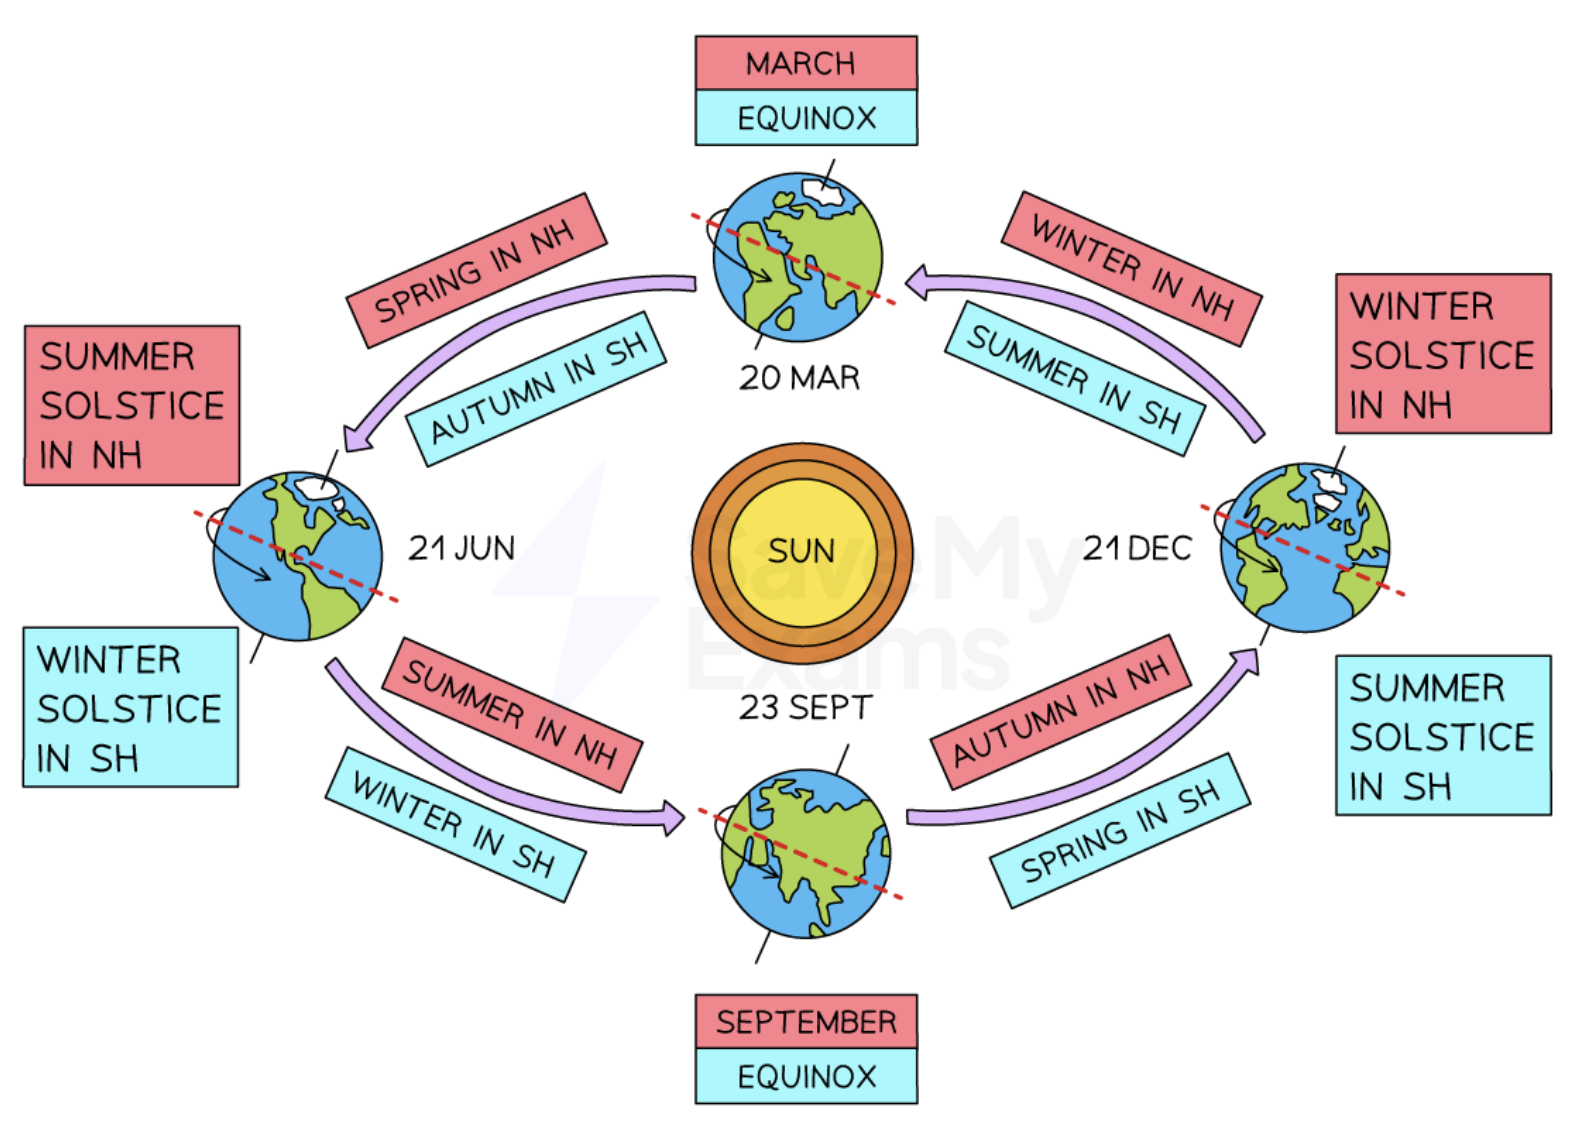
\includegraphics[width=0.8\linewidth]{截圖 2026-02-11 22.53.14.png}
\end{center}
The Moon is a natural satellite that orbits around the Earth in a roughly circular orbit; takes about one month (28 days) to complete one orbit; and rotates on its axis once every 28 days so the same side always faces the Earth. It is visible in the night sky because it reflects the light from the Sun.\\
\begin{center}
    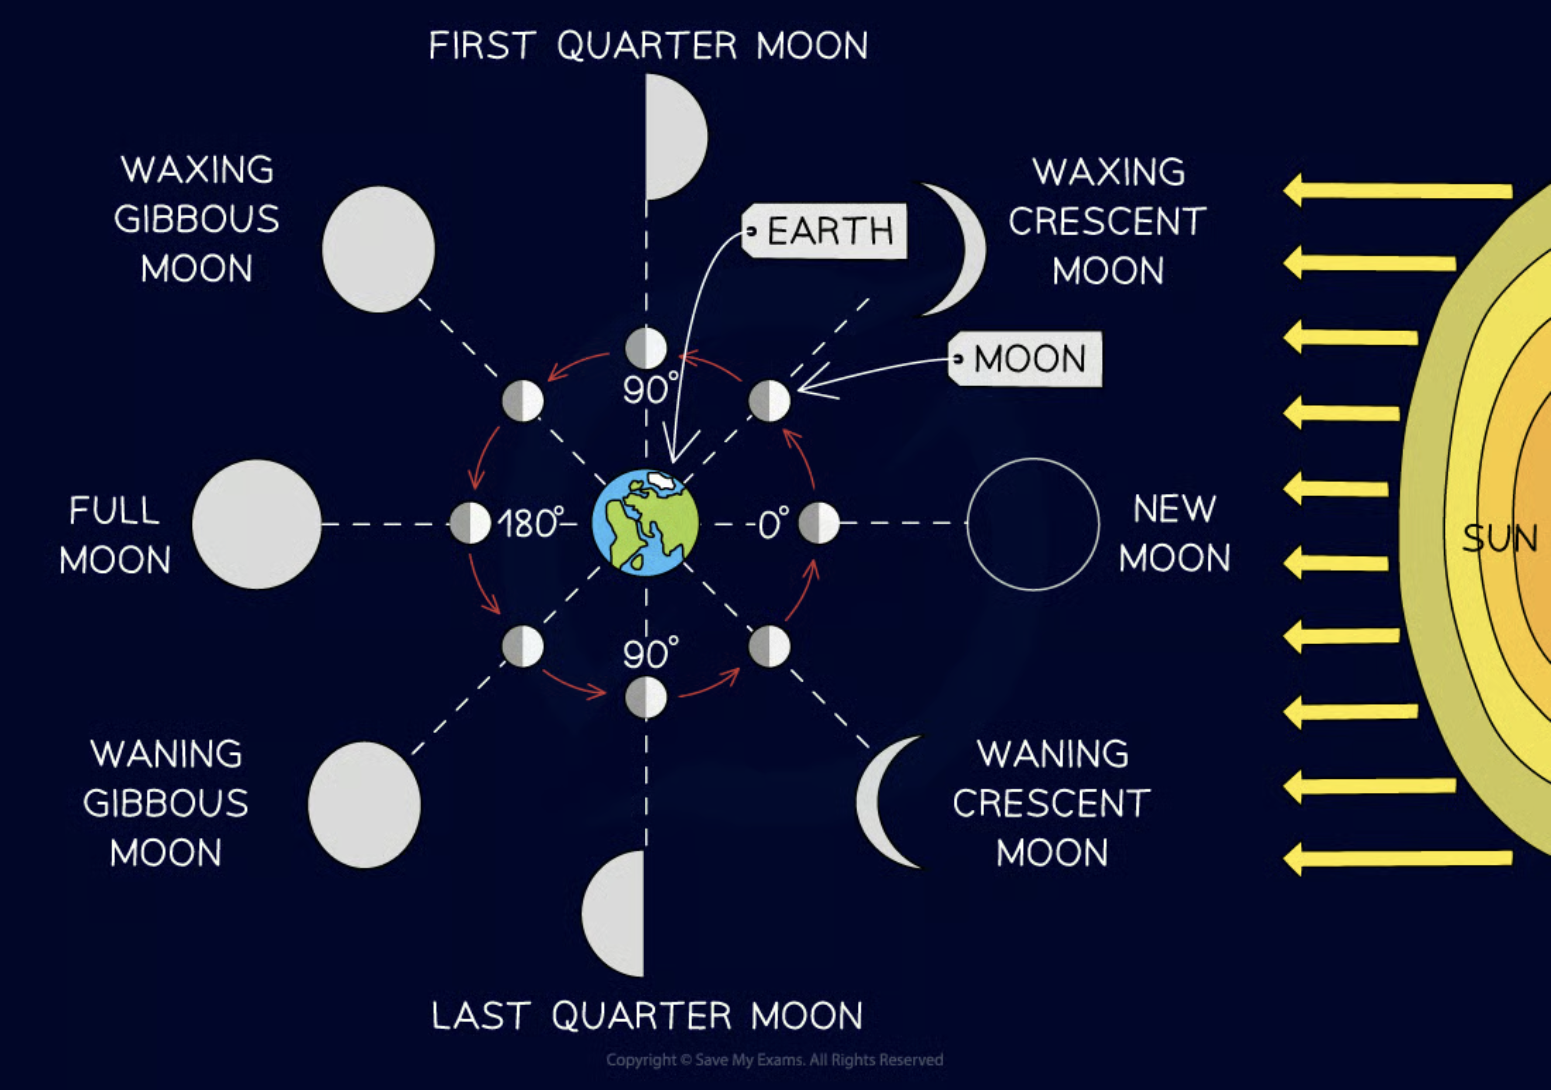
\includegraphics[width=0.7\linewidth]{截圖 2026-02-11 22.54.52.png}
\end{center}
The Solar System consists of the Sun, eight planets, natural \& artificial satellites, dwarf planets, asteroids and comets.
\begin{center}
    \textbf{Mercury, Venus, Earth, Mars, Jupiter, Saturn, Uranus, Neptune.}\\
    These are the eight planets in the Solar System.\\
    They are either \textbf{the inner rocky planets} (rocky, small, with atmosphere) \\\textit{or}\\ \textbf{the outer gas giants} (gaseous, large, made out of \(H_2\ \&\ He\)).
\end{center}
A dwarf planet is an object similar to a planet, but much smaller. \\The gravitational field around a dwarf planet is not strong enough to pull in nearby objects.\\\\
Natural satellites are objects that orbit planets. \\Artificial satellites are manmade objects that orbit another object in space.\\\\
Asteroids (small rocky objects) and comets (objects made of dust and ice, have elliptical orbits) also orbit the Sun.\\\\
\textbf{The formation of the solar system is as follows:}
\begin{enumerate}
    \item The Sun and the planets in the Solar System formed from a cloud of dust and gas / nebula.
    \item In the nebula, matter accreted, which means attractive gravitational forces between particles caused them to join together and grow into larger objects.
    \item Gravity pulled this cloud together into a giant ball, which would eventually become the Sun.
    \item As the nebula collapsed, it began to spin faster, became hotter, and formed an accretion disc.
    \item From the rotating accretion disc, the Sun and the planets emerged.
    \item The Solar System then formed around 4.5 billion years ago.
    \item The planets formed from the remnants of the matter left over from the nebula that formed the Sun, which contained many elements that were created during a supernova explosion in the distant past. 
    \item As the early Sun became hotter, gaseous matter was pushed further out into the Solar System than solid matter.
    \item For inner rocky planets:
    \begin{itemize}
        \item The inner planets formed from materials with high melting temperatures such as metals; this is caused by the high temperature.
        \item The original nebula contained only a small proportion of heavy elements, so the inner planets could not grow as significantly as the outer planets.
        \item As a result, solids in the inner disc were pulled together by gravity to form solid planets.
    \end{itemize}
    \item For outer gas giants:
    \begin{itemize}
        \item In the cooler regions, further from the Sun, the temperature was low enough for the light molecules to exist in a solid state.
        \item Therefore, the outer planets formed from materials with low melting temperatures.
        \item The original nebula contained a large proportion of light elements, so the outer planets were able to become exceptionally large.
        \item As a result, gases in the outer disc were pulled together by gravity to form gaseous planets.
    \end{itemize}
\end{enumerate}
\newpage 
Light speed is equal to \(3.0\times 10^8\ m/s\). (I know no one cares)\\\\
The strength of a gravitational field around a planet depends on the \(m\) of the planet \& the distance from the planet.\\
The greater the mass of a planet, the greater the strength of the gravitational field at its surface.\\
As the distance from a planet increases, the strength of the gravitational field decreases.\\\\
For objects orbiting around the Sun, the Sun's gravitational attraction keeps them in orbit \& the force is directed from the orbiting object to the center of the Sun.\\
The further a planet is from the Sun, the smaller its orbital speed \& the longer its orbital period.\\\\
The orbital speed for a planet is given by: (Assuming the orbit is circular)
\[v=\frac{2\pi r}{T}\]
where \(T\) is the orbital period, the time taken for an object to complete one orbit.\\\\
Try this extension formula if you're interested:
\[v=\sqrt{\frac{GM}{r}},\ \text{where}\ G=6.67 \times 10^{-11}\ N\times m^2/kg^2\]
The orbits of planets, minor planets and comets are elliptical (especially comets).\\
As the comet \textbf{approaches} the Sun, the \(r\) of the orbit decreases, the \(v\) increases due to the Sun's strong gravitational pull. It has greater \(E_k\) kinetic energy (causing it to speed up) \& less GPE.\\
As the comet \textbf{travels further away} from the Sun, the \(r\) of the orbit increases, the \(v\) decreases due to a weaker gravitational pull. It has less \(E_k\) kinetic energy (causing it to slow down) \& more GPE.\\
Conservation of energy in elliptical orbits, isn't it?
\subsection{Stars \& the Universe: what's in that?}
The Sun is a medium-sized star which lies at the centre of the Solar System. It consists mostly of the two elements: \(H\ \&\ He\).\\
It radiates most of its energy in the IR, visible and UV regions of the EM spectrum.\\
In the centre of a star, \(H\) nuclei undergo nuclear fusion to form \(He\) nuclei. A huge amount of energy is released in the reaction. 
All stable stars are powered by nuclear fusion reactions. \\\\
Some \textit{professional vocabs} about the universe:
\begin{itemize}
    \item The Universe: A large collection of billions of galaxies / the entirety of space
    \item Galaxy: A large collection of billions of stars (e.g. the Milky Way)
    \item Astronomical Units: The distance travelled by light in one year, \(9.5\times 10^{15}\ m\)
\end{itemize}
\newpage
\subsubsection{Star Formation: the ultimate diagram}
\begin{center}
    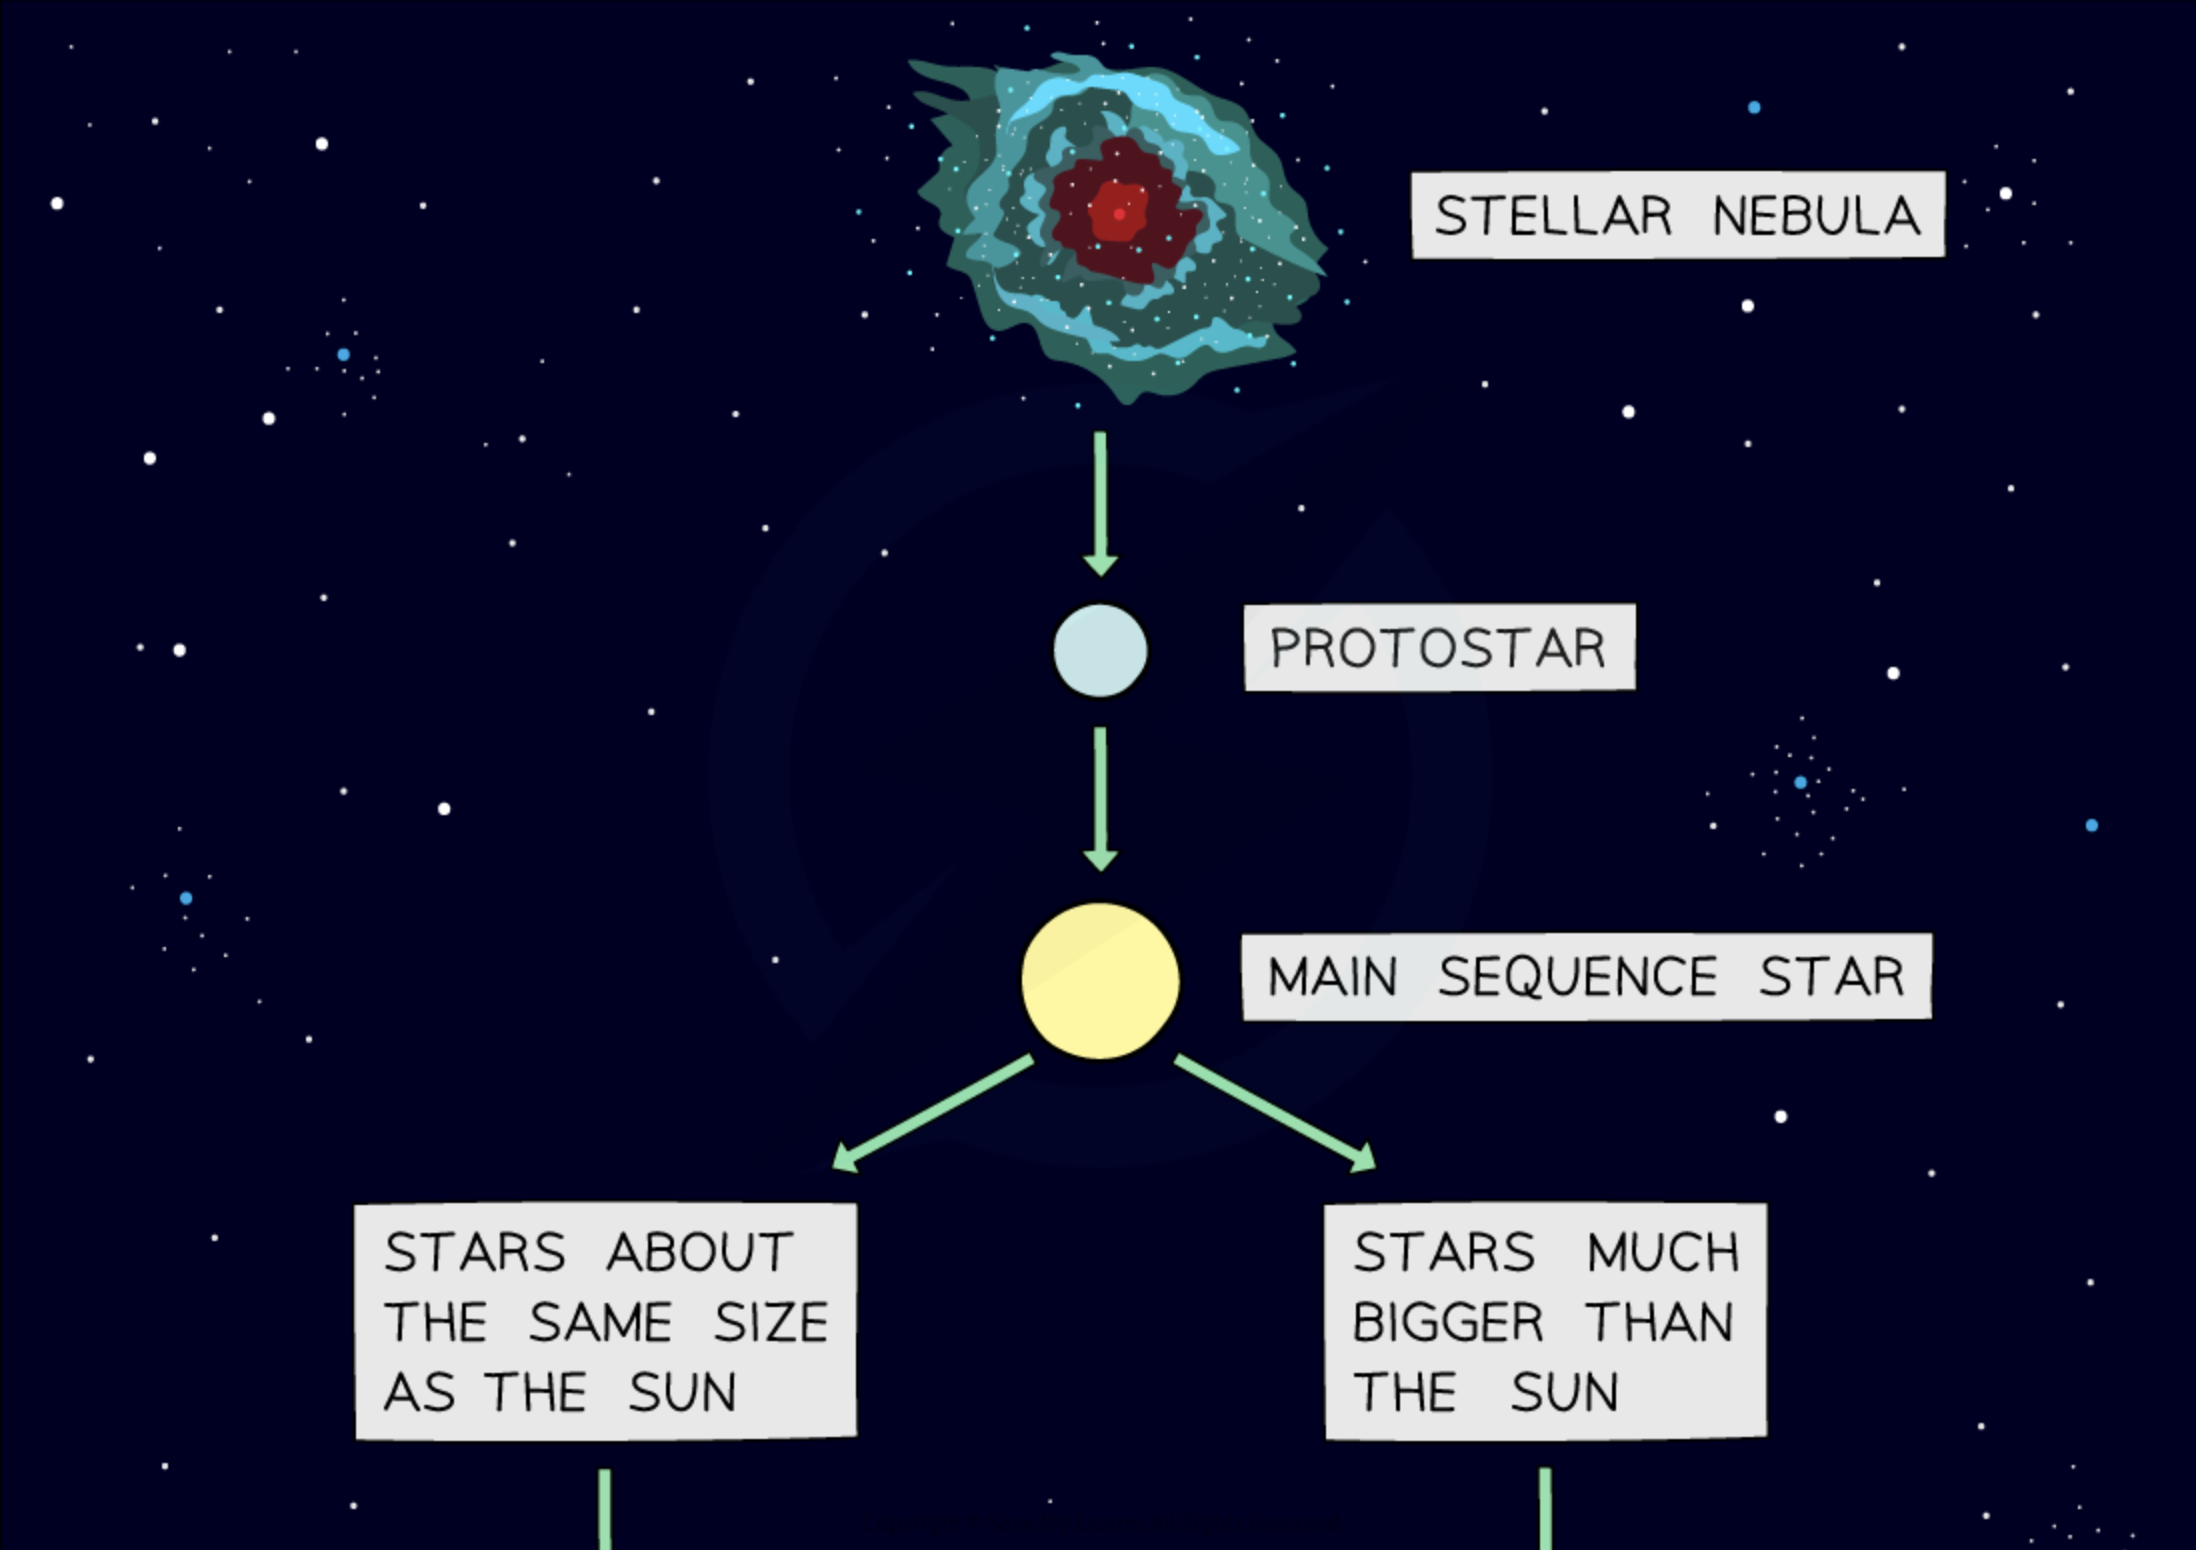
\includegraphics[width=0.9\linewidth]{截圖 2026-02-11 23.27.00.png}\\
    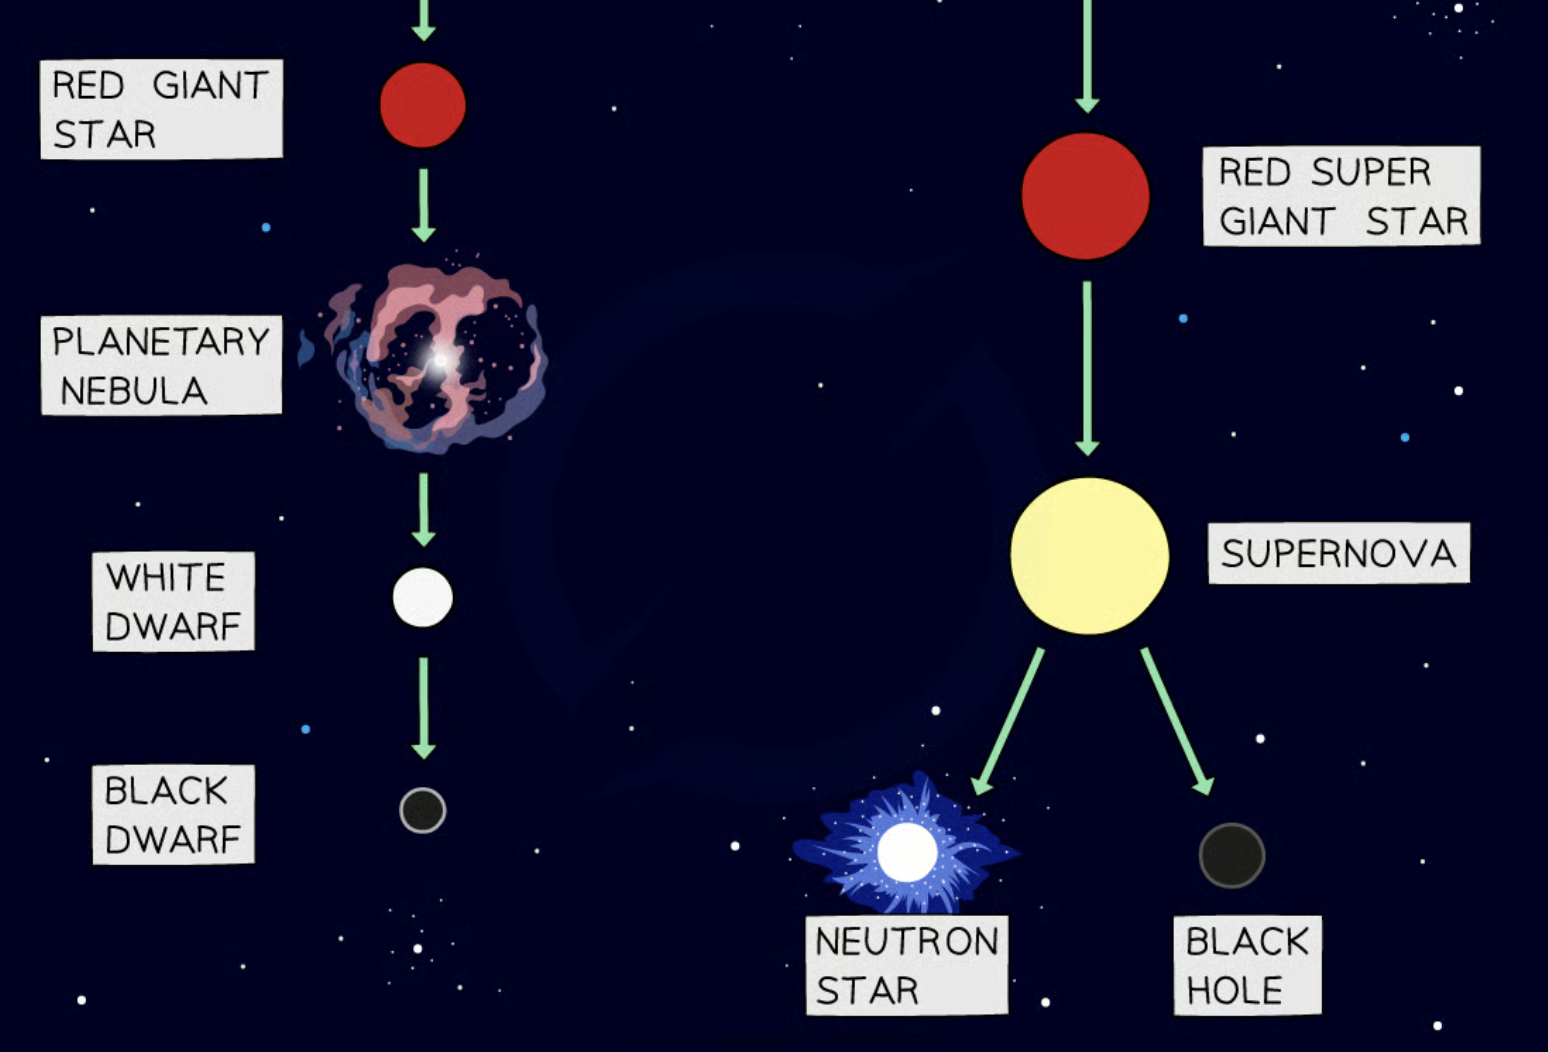
\includegraphics[width=0.9\linewidth]{截圖 2026-02-11 23.27.18.png}
\end{center}
\textbf{Note:} Stars form from a giant interstellar cloud of gas and dust called a nebula.\\
The gravitational attraction within a nebula pulls the particles closer together until a hot ball of gas forms, known as a protostar. 
Once the protostar becomes hot enough, nuclear fusion reactions occur within its core. (Stable star period)
The outward (thermal due to energy released) and inward (pull of gravity) forces within a stable star are in equilibrium.\\
The final stages of its life cycle depend on its mass.\\
For Low-mass stars:
\begin{itemize}
    \item After several billion years, the \(H_2\) fuel used for nuclear reactions begins to run out.
    \item Once this happens, the rate of fusion decreases, which causes the core to shrink and heat up.
    \item As the energy produced by fusion decreases, the inward force due to gravity becomes greater than the outward force due to the thermal pressure.
    \item Eventually, the star becomes a red giant when the core becomes hot enough for \(He\) to fuse into \(C\).
    \item The energy released by re-ignited fusion reactions causes the outer layers of the star to expand and cool.
    \item Once the \(He\) in the core runs out, fusion reactions cannot continue.
    \item The star becomes unstable and the core collapses under its own gravity.
    \item The outer layers are ejected into space as a planetary nebula.
    \item The collapsed core of the red giant is called a white dwarf.
    \item The white dwarf cools down over time and as a result, the amount of energy it emits decreases.
\end{itemize}
For High-mass stars:
\begin{itemize}
    \item After several million years, the \(H_2\) in the core begins to run out.
    \item Similar to a low-mass star, the rate of fusion decreases and the core shrinks and heats up.
    \item The star becomes a red supergiant when the core becomes hot enough for \(He\) fusion to start.
    \item This causes the outer layers of the star to expand and cool.
    \item During this stage, the core collapses and expands repeatedly as fusion reactions start and stop.
    \item Eventually, fusion reactions inside the red supergiant cannot continue once iron is formed.
    \item The core of the star will collapse rapidly and initiate a gigantic explosion called a supernova.
    \item At the centre of this explosion, a dense body called a neutron star will form.
    \item The outer layers of the star are ejected into space forming new nebulas.
    \item In the case of the most massive stars, the neutron star that forms at the centre will continue to collapse under the force of gravity until it forms a black hole.
\end{itemize}
\subsubsection{Redshift: Change in \(\lambda\)}
If a source of light moves away from an observer, the observed \(\lambda\) increases, shifts towards the red end of the spectrum, called \textbf{redshift}.\\
Vice Versa: If a source of light moves towards an observer, the observed \(\lambda\) decreases, shifts towards the blue end of the spectrum, called blueshift.\\
When astronomers compare light from glowing \(H_2\) in distant galaxies with light from glowing \(H_2\) on Earth, the light appears to be redshifted. 
This means the observed \(\lambda\) has increased as the light travelled from the galaxy to the Earth. This shows that \textbf{distant stars and galaxies are moving away (receding) from the Earth}. 
Greater redshift, greater distance apart \& greater speed.
\newpage
\subsubsection{Big BBAANG!!! \& Hubble Constant \(H_0\)}
Around 14 billion years ago, the Universe began from a single point that was extremely hot and dense. A giant explosion, known as \textbf{the Big Bang}, caused the Universe to expand outwards.
As each point moved away from the others, the Universe began to cool.
As a result of the initial explosion, the Universe continues to expand.\\
\textbf{Proof:}
\begin{itemize}
    \item \textbf{Galactic redshift} indicates that distant galaxies are moving away from us. This means the Universe must be expanding.
    \item \textbf{Cosmic Microwave Background Radiation (CMBR)}:
    \begin{itemize}
        \item Form of EM radiation that was emitted shortly after the beginning of the Universe. It is detected everywhere throughout the Universe.
        \item Big Bang Theory predicts the early Universe was extremely hot and dense: CMBR changed from short \(\lambda\ \gamma\) radiation \(\to\) long \(\lambda\) microwave radiation (redshifted). CMBR is consistent with radiation (left over from Big Bang) that has been stretched over time.
        \item This is because the Universe has expanded and cooled, causing the \(\lambda\) to increase.
        \item This suggests the Universe was initially very small and very energetic and has been expanding since.
    \end{itemize}
\end{itemize}
\textbf{Hubble's law states that the speed of recession is proportional to the distance of the galaxy away from Earth.}, \(v \propto d\). 
This means that the further away a galaxy is from Earth, the faster it is moving away \& the greater the increase in redshift.\\\\
The Hubble Constant \(H_0\) is defined as the ratio of the speed at which the galaxy is moving away from the Earth, to its distance from the Earth.
\[H_0\ (s^{-1})=\frac{v\ (km/s)}{d\ (km)};\ v=H_0d\]
\begin{center}
    Remember the value of the Hubble Constant \(H_0\): \(2.2\times 10^{-18}\ s^{-1}\)
\end{center}
The Hubble Constant \(H_0\) can be determined from measurements of redshift (change in \(\lambda\)) of the light emitted by a galaxy / the brightness of supernova in the galaxy.\\\\
The age of the Universe (a rough estimate using \(H_0\)) is given by:
\[\frac{1}{H_0}=\frac{d}{v}\]
since time equals \(\frac{d}{v}\), \(\frac{1}{H_0}\approx 14\ \text{billion years}\).\\
\newpage
\section{Final surprise(s)}
\begin{center}
    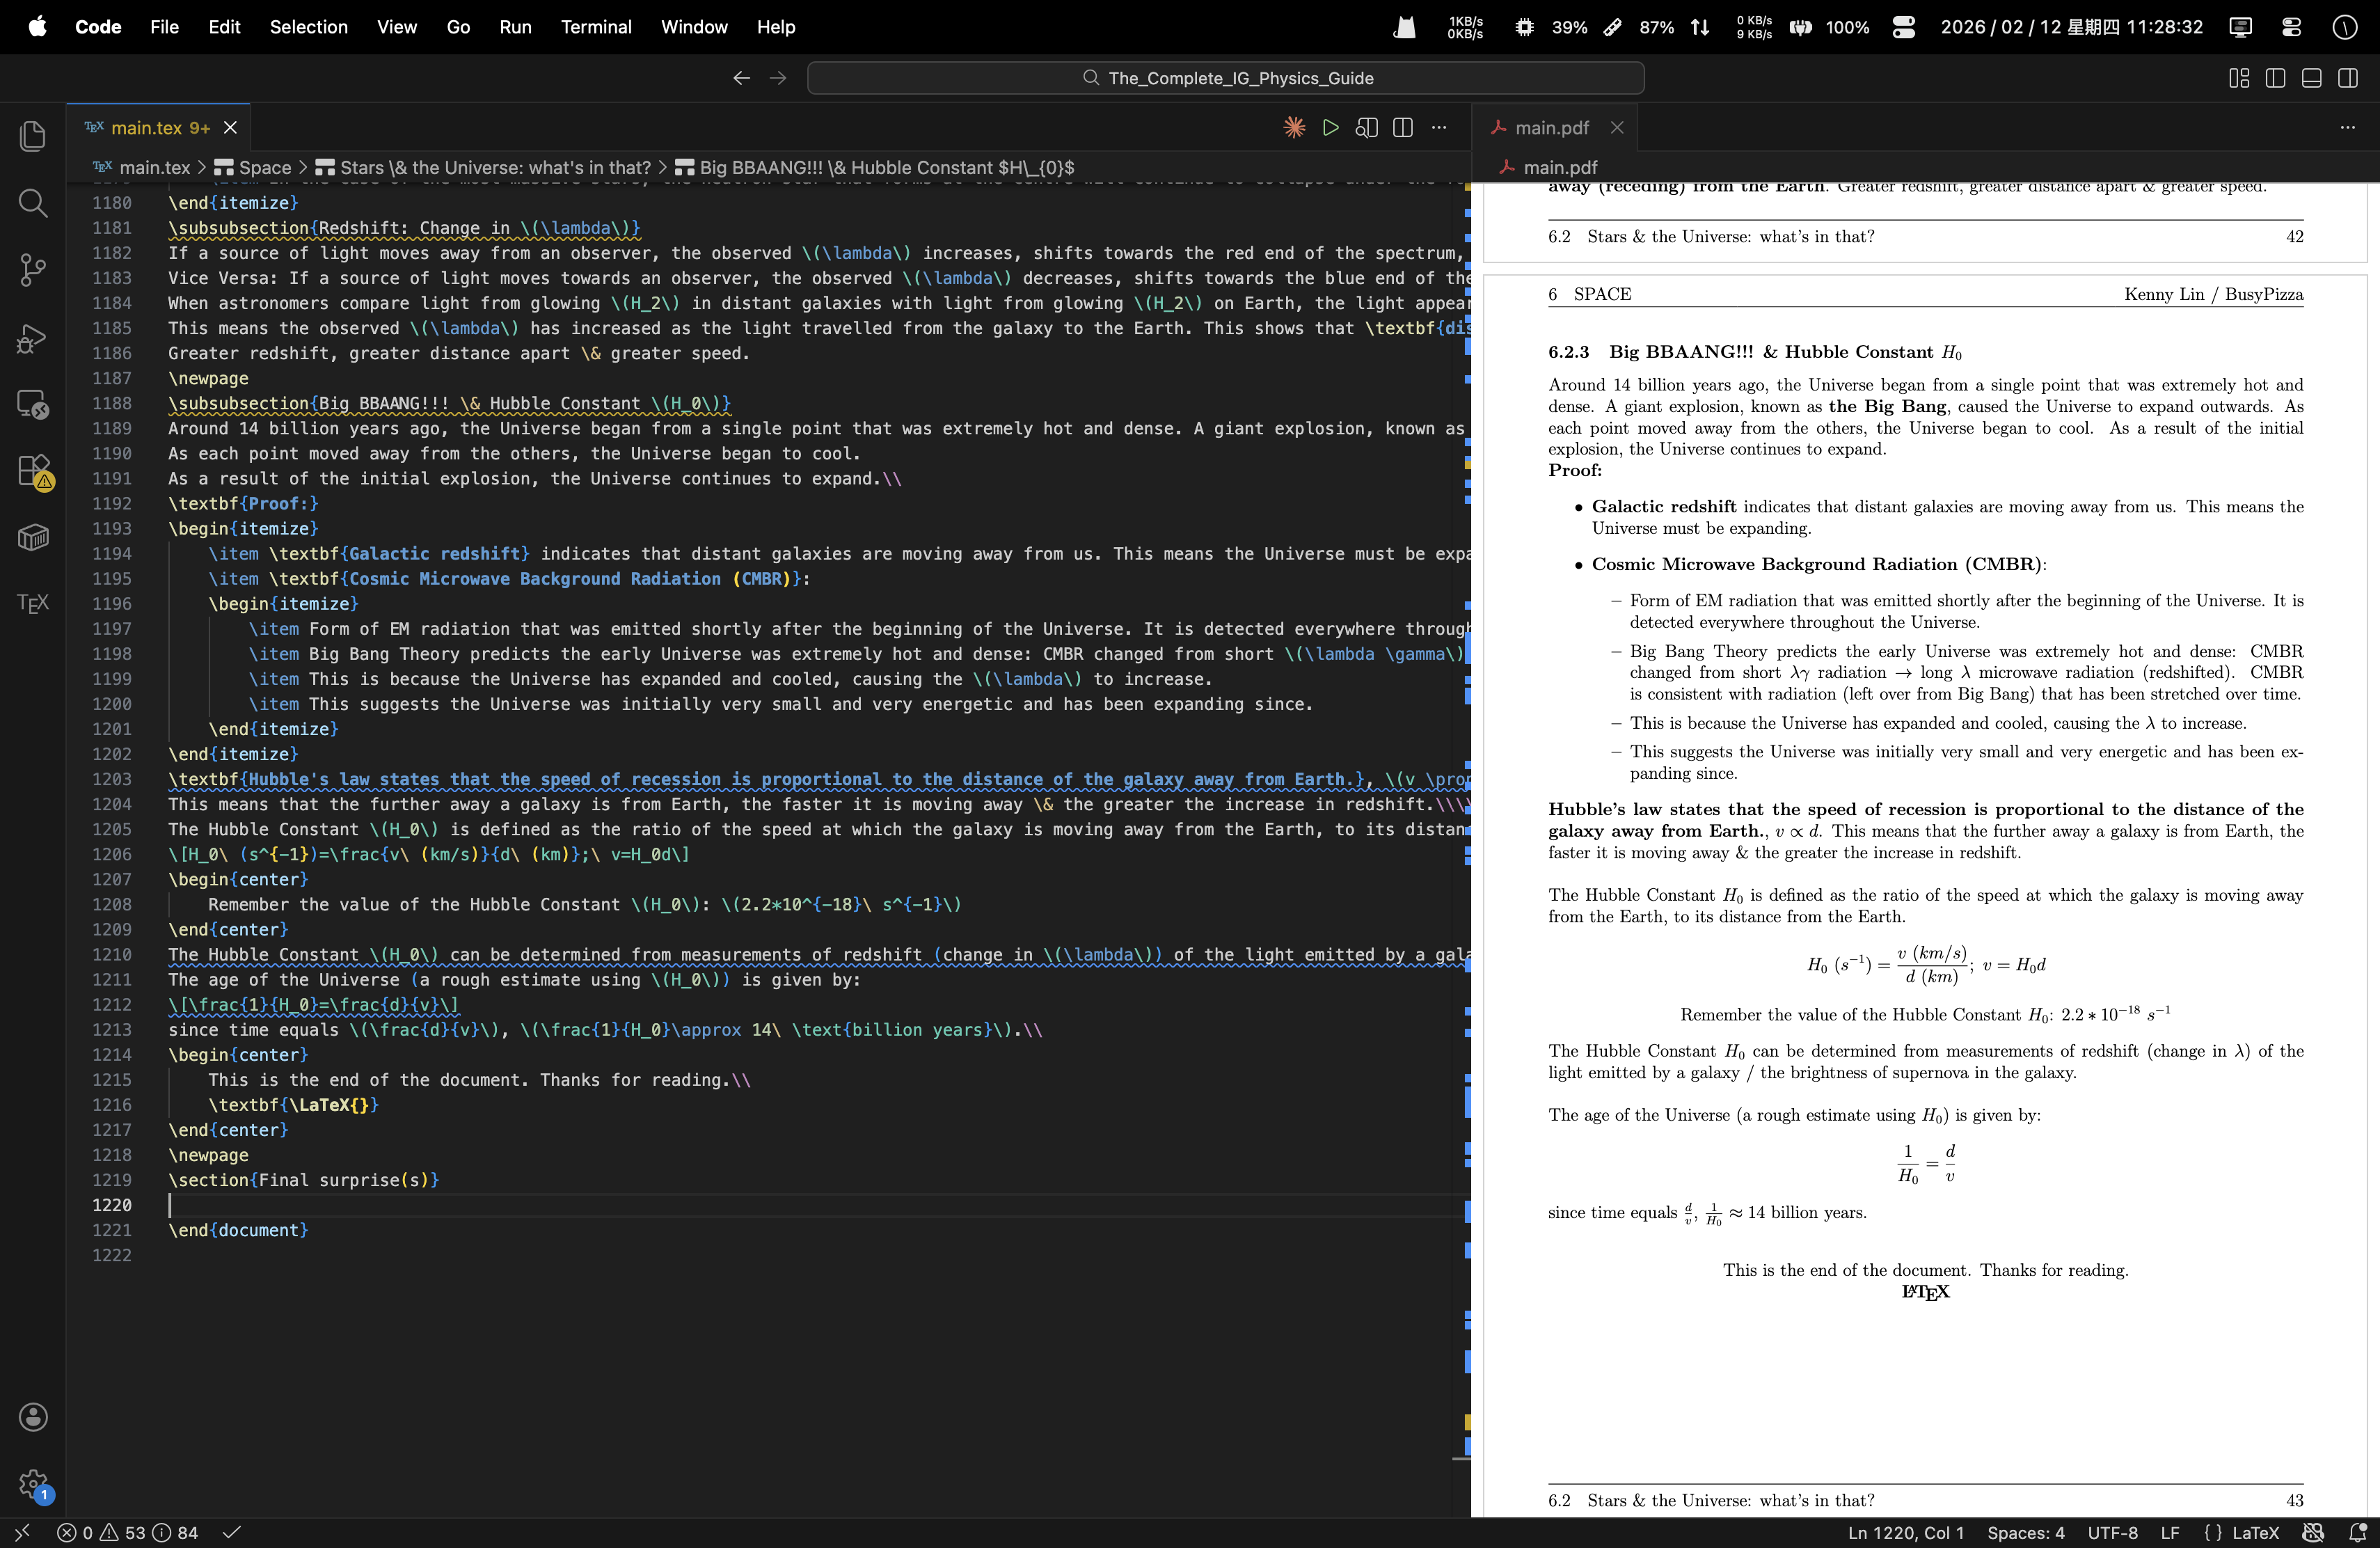
\includegraphics[width=1\linewidth]{截圖 2026-02-12 11.28.32.png}\\
    Everyone! Go try out Visual Studio Code! Now!\\
    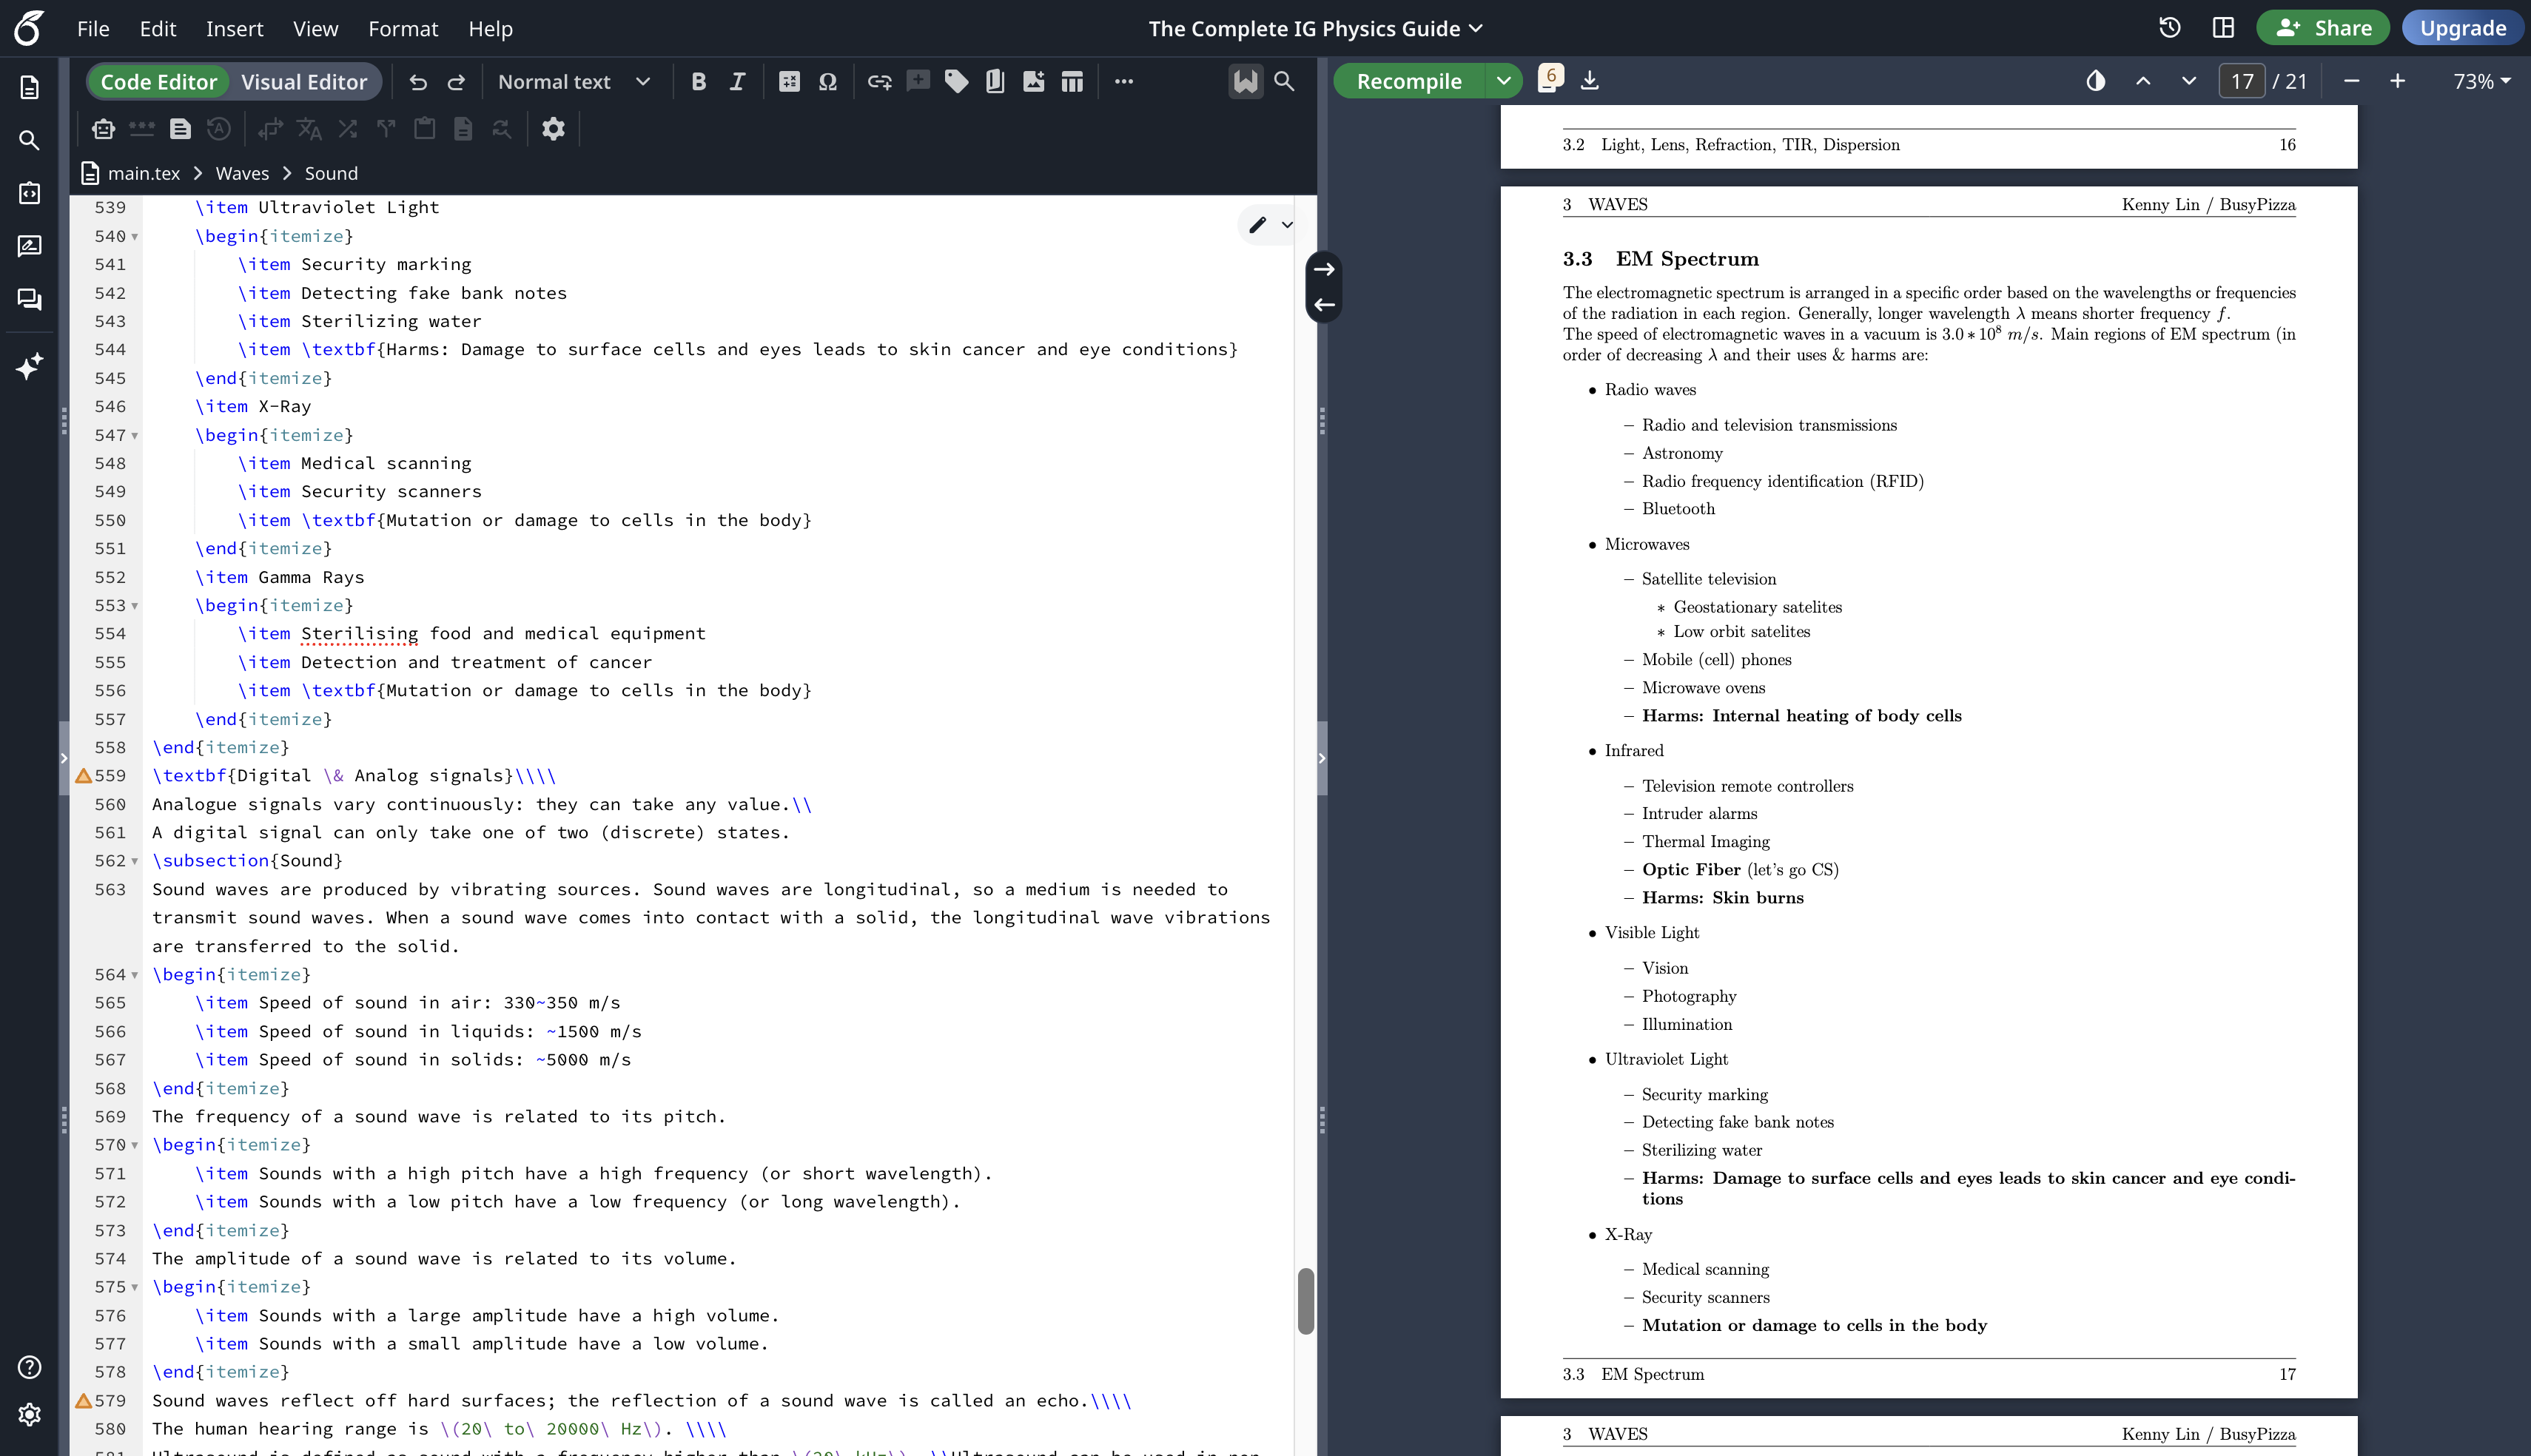
\includegraphics[width=1\linewidth]{截圖 2026-02-12 11.31.16.png}\\
    Also go try Overleaf if you're interested. \\(Although I encountered some bugs that made my computer SUPER hot)\\
    Finally, use \LaTeX{} because it's cool! The experience is just like typing code.
\end{center}
\end{document}
